\chapter{Validación de Herramientas Numéricas} \label{cap:validacion}


En este capítulo se pretende validar y asegurar el correcto funcionamiento de las \linebreak herramientas numéricas utilizadas. El mismo se divide en dos partes. Una primera parte que se centra en validar la herramienta de simulaciones DNS, Xcompact3D. Para tal fin se emplean diferentes mallas (o resoluciones) espaciales y pasos temporales según se requiera. En la segunda parte de este capítulo se valida la herramienta generadora de autovalores y autofunciones, OSMC. 

Se emplean tres situaciones diferentes para validar XC3D: (i) un canal de placas paralelas en régimen turbulento con flujo de calor constante en las paredes, donde se analizan aspectos hidrodinámicos y térmicos para convección forzada \cite{moser1999, kawamura2000dns}; (ii) mismo sistema físico que el caso anterior pero en régimen laminar, teniendo en cuenta el acople de las ecuaciones de conservación debido al término de fuerza boyante \linebreak \cite{chen1996linear}; (iii) canal vertical de placas paralelas isotérmicas a distinta temperatura entre sí, en régimen  turbulento con convección mixta \cite{guo2022direct}. En los casos turbulentos se analiza la convergencia en malla y la opción computacionalmente más económica que satisfaga una precisión aceptable.

La corroboración de la herramienta numérica OSMC se realiza en dos etapas: (i) se ratifica que OSMC genere los autovalores correctos, para eso se considera la variación de la parte \linebreak imaginaria del autovalor más inestable en función del número de onda \cite{chen1996linear}; (ii) se corrobora que las autofunciones entregadas por el código sean correctas y para ello se utiliza como referencia autofunciones asociadas a ondas 2D y 3D \cite{chen2003direct}.

Adicionalmente, las predicciones producidas por la teoría de estabilidad lineal, sobre la evolución temporal de ciertas magnitudes de interés, se comparan con aquellos resultados obtenidos vía simulaciones DNS. En general, se observa que las herramientas empleadas \linebreak responden adecuadamente y son consistentes con los datos de referencia.



\newpage
 
\section{Primera Parte: Xcompact3D}

En esta sección se presentan los resultados obtenidos con la herramienta numérica \linebreak Xcompact3D (XC3D) para un canal de placas paralelas en flujo completamente desarrollado. Para la validación de XC3D se consideran las siguientes situaciones de flujo: 

\begin{itemize}

\item \textbf{Situación I:} flujo turbulento hidrodinámico y completamente desarrollado,

\item \textbf{Situación II:} flujo turbulento hidrodinámica y térmicamente desarrollado con flujo de calor constante en las paredes, considerando únicamente convección forzada.

\item \textbf{Situación III:} flujo en régimen laminar hidrodinámica y térmicamente desarrollado con flujo de calor constante en las paredes donde se considera el efecto de la fuerza boyante, es decir, en régimen de convección mixta; 

\item \textbf{Situación IV:} por último, se considera un canal turbulento completamente desarrollado (hidrodinámica y térmicamente) con convección mixta cuyas paredes están sometidas a una diferencia de temperatura constante. 

\end{itemize}
En cada una de las situaciones expuestas, los resultados se comparan con datos de referencia.

A lo largo de la etapa de validación, para las distintas simulaciones DNS realizadas, se emplearon distintas resoluciones espaciales y pasos temporales, las cuales se especifican en la Tabla \ref{tab:meshes}. Asimismo, en dicha tabla se expresan la cantidad de nodos utilizados en las direcciones $X$, $Y$ y $Z$ (N$_x$, N$_y$ y N$_z$, respectivamente). Nótese, además, que la discretización empleada en la dirección $Y$ es no uniforme. El dominio utilizado en todas las simulaciones corresponde a L$_x \times$ L$_y \times$ L$_z$ = $8 \times 2 \times 4$.

Por otro lado, en cada simulación (según se requiera) se imponen los parámetros Re$_o$, Pr y/o Ri$_b$. Posteriormente, se deja evolucionar el sistema hasta que los campos asociados alcancen el estado estadísticamente estacionario. Una vez en dicho estado, se colecta estadística por al menos 500 unidades temporales. Para acelerar la obtención del estado turbulento, XC3D cuenta con la capacidad de introducir  ruido aleatorio, y/o también rotación\footnote{La rotación se logra agregando un término asociado a la fuerza de Coriolis en la ecuación de momento \cite{lamballais2014}, que viene implementada en el propio código.} en el propio flujo. 

Las simulaciones se realizan en el \textit{cluster ``mecclust''} del grupo MECOM (CAB-CNEA). Dependiendo de la disponibilidad y de la exigencia demandada, cada simulación se puede \linebreak correr en un nodo individual de los veinte disponibles, los cuales emplean 2 procesadores \textit{Xeon E5 2660 V3 @2.6 GHz} con 10 \textit{cores} cada uno; o también, si se requiere, es posible utilizar cuatro nodos con conexión \textit{InfiniBand} que da un total de 80 \textit{cores}. Para aquellas simulaciones más demandantes, el número mínimo de pasos temporales por hora es aproximadamente 800, y el almacenamiento requerido puede alcanzar los 100 GB. Para dar una idea general del \textit{wall-clock} requerido, empleando 20 \textit{cores}, una simulación de 500 unidades temporales con la malla M0 (véase Tabla \ref{tab:meshes}) puede tardar del orden de 35 minutos mientras que una simulación idéntica con la malla M4 puede requerir del orden de 670 horas.       


\begin{table}[H]
\centering
\resizebox{0.7\textwidth}{!}{%
\begin{tabular}{lcccc}
\toprule
Nomenclatura & N$_x \times$ N$_y \times$ N$_z$ & $(\Delta x^*,\Delta y^*_{\text{max}},\Delta z^*)$ & $\Delta t^*$ \\
\midrule
M0 & $64 \times 65 \times 64$    & (0.125, 0.087, 0.062) & 0.005 \\
M1 & $128 \times 65 \times 64$   & (0.062, 0.087, 0.062) & 0.005 \\
M2 & $128 \times 129 \times 128$ & (0.062, 0.044, 0.031) & 0.002 \\
M3 & $160 \times 161 \times 160$ & (0.05,  0.035, 0.025)  & 0.001 \\
M4 & $256 \times 257 \times 256$ & (0.031, 0.022, 0.015)  & 0.001 \\
\bottomrule
\end{tabular}}
\caption{Distintas resoluciones espaciales y temporales utilizadas en las simulaciones de validación. Debido a que la discretización en la dirección $Y$ es no uniforme, se reporta el máximo $\Delta y$ asociado.}
\label{tab:meshes}
\end{table}

Algunos resultados, presentes en esta primera parte, se encuentran adimensionalizados en unidades de pared (indicadas con el superíndice ``+'') basadas en el semiancho del canal $d$, la velocidad de fricción $u_{\tau}$ y la temperatura de fricción $T_{\tau}$:

\begin{itemize}
	\item Esfuerzo de Corte: $\tau_w= \mu_o \partial u_x / \partial y$ (evaluada en $y=\pm d$)  
	\item $u_{\tau} = \sqrt{\tau_w / \rho}$ ; $T_{\tau}=\frac{q''_w}{\rho c_p u_{\tau}}$
	\item $\mathbf{u}^+ = \mathbf{u} / u_{\tau}$ ; $\theta^+ = \theta / T_{\tau}$ ; $y^+ = \frac{u_{\tau} y}{\nu_o}$
\end{itemize}
Por otro lado, los perfiles de las magnitudes seleccionadas se encuentran promediadas en la dirección X y Z, y en el tiempo.

\subsection{Situación I. Canal turbulento (sólo hidrodinámica)}

En esta subsección se exponen los resultados del canal turbulento considerando los \linebreak aspectos hidrodinámicos únicamente. En este caso se impone Re$_o$=4200 y se realizan \linebreak simulaciones para las mallas M0, M1, M2 y M3.  

En las Figuras \ref{fig:kim-ux} - \ref{fig:kim-uxuy} se presentan (respectivamente) algunas magnitudes de interés para este sistema: el perfil de velocidad \textit{streamwise} $\langle u^+_x \rangle$ y los perfiles de las componentes del tensor de Reynolds\footnote{Sea $R_{ij} = \langle u^{\prime}_i u^{\prime}_j \rangle$ el tensor de Reynolds, entonces: la raíz cuadrada de la componente diagonal $R_{ii}$ coincide con el valor rms de la fluctuación de velocidad en la dirección $i$-ésima. Esto es, $(u_i)_{rms} = \sqrt{R_{ii}}$.} $\sqrt{\langle u^{+ \prime}_x u^{+ \prime}_x \rangle}$, $\sqrt{\langle u^{+ \prime}_y u^{+ \prime}_y \rangle}$ y $\langle u^{+ \prime}_x u^{+ \prime}_y \rangle$. En estas gráficas se comparan las distintas mallas empleadas con el trabajo de Moser \textit{et al.} \cite{moser1999}. Al refinar la malla (M0$\rightarrow$M3), las cantidades de interés se estabilizan; entre M2 y M3 las diferencias son prácticamente despreciables. Por lo tanto, se considera alcanzada la independencia de malla. Con esa resolución, los resultados DNS de XC3D muestran buen acuerdo con los datos de referencia.

\newpage

\begin{figure}[H]
 \centering
    \subfloat[]{
    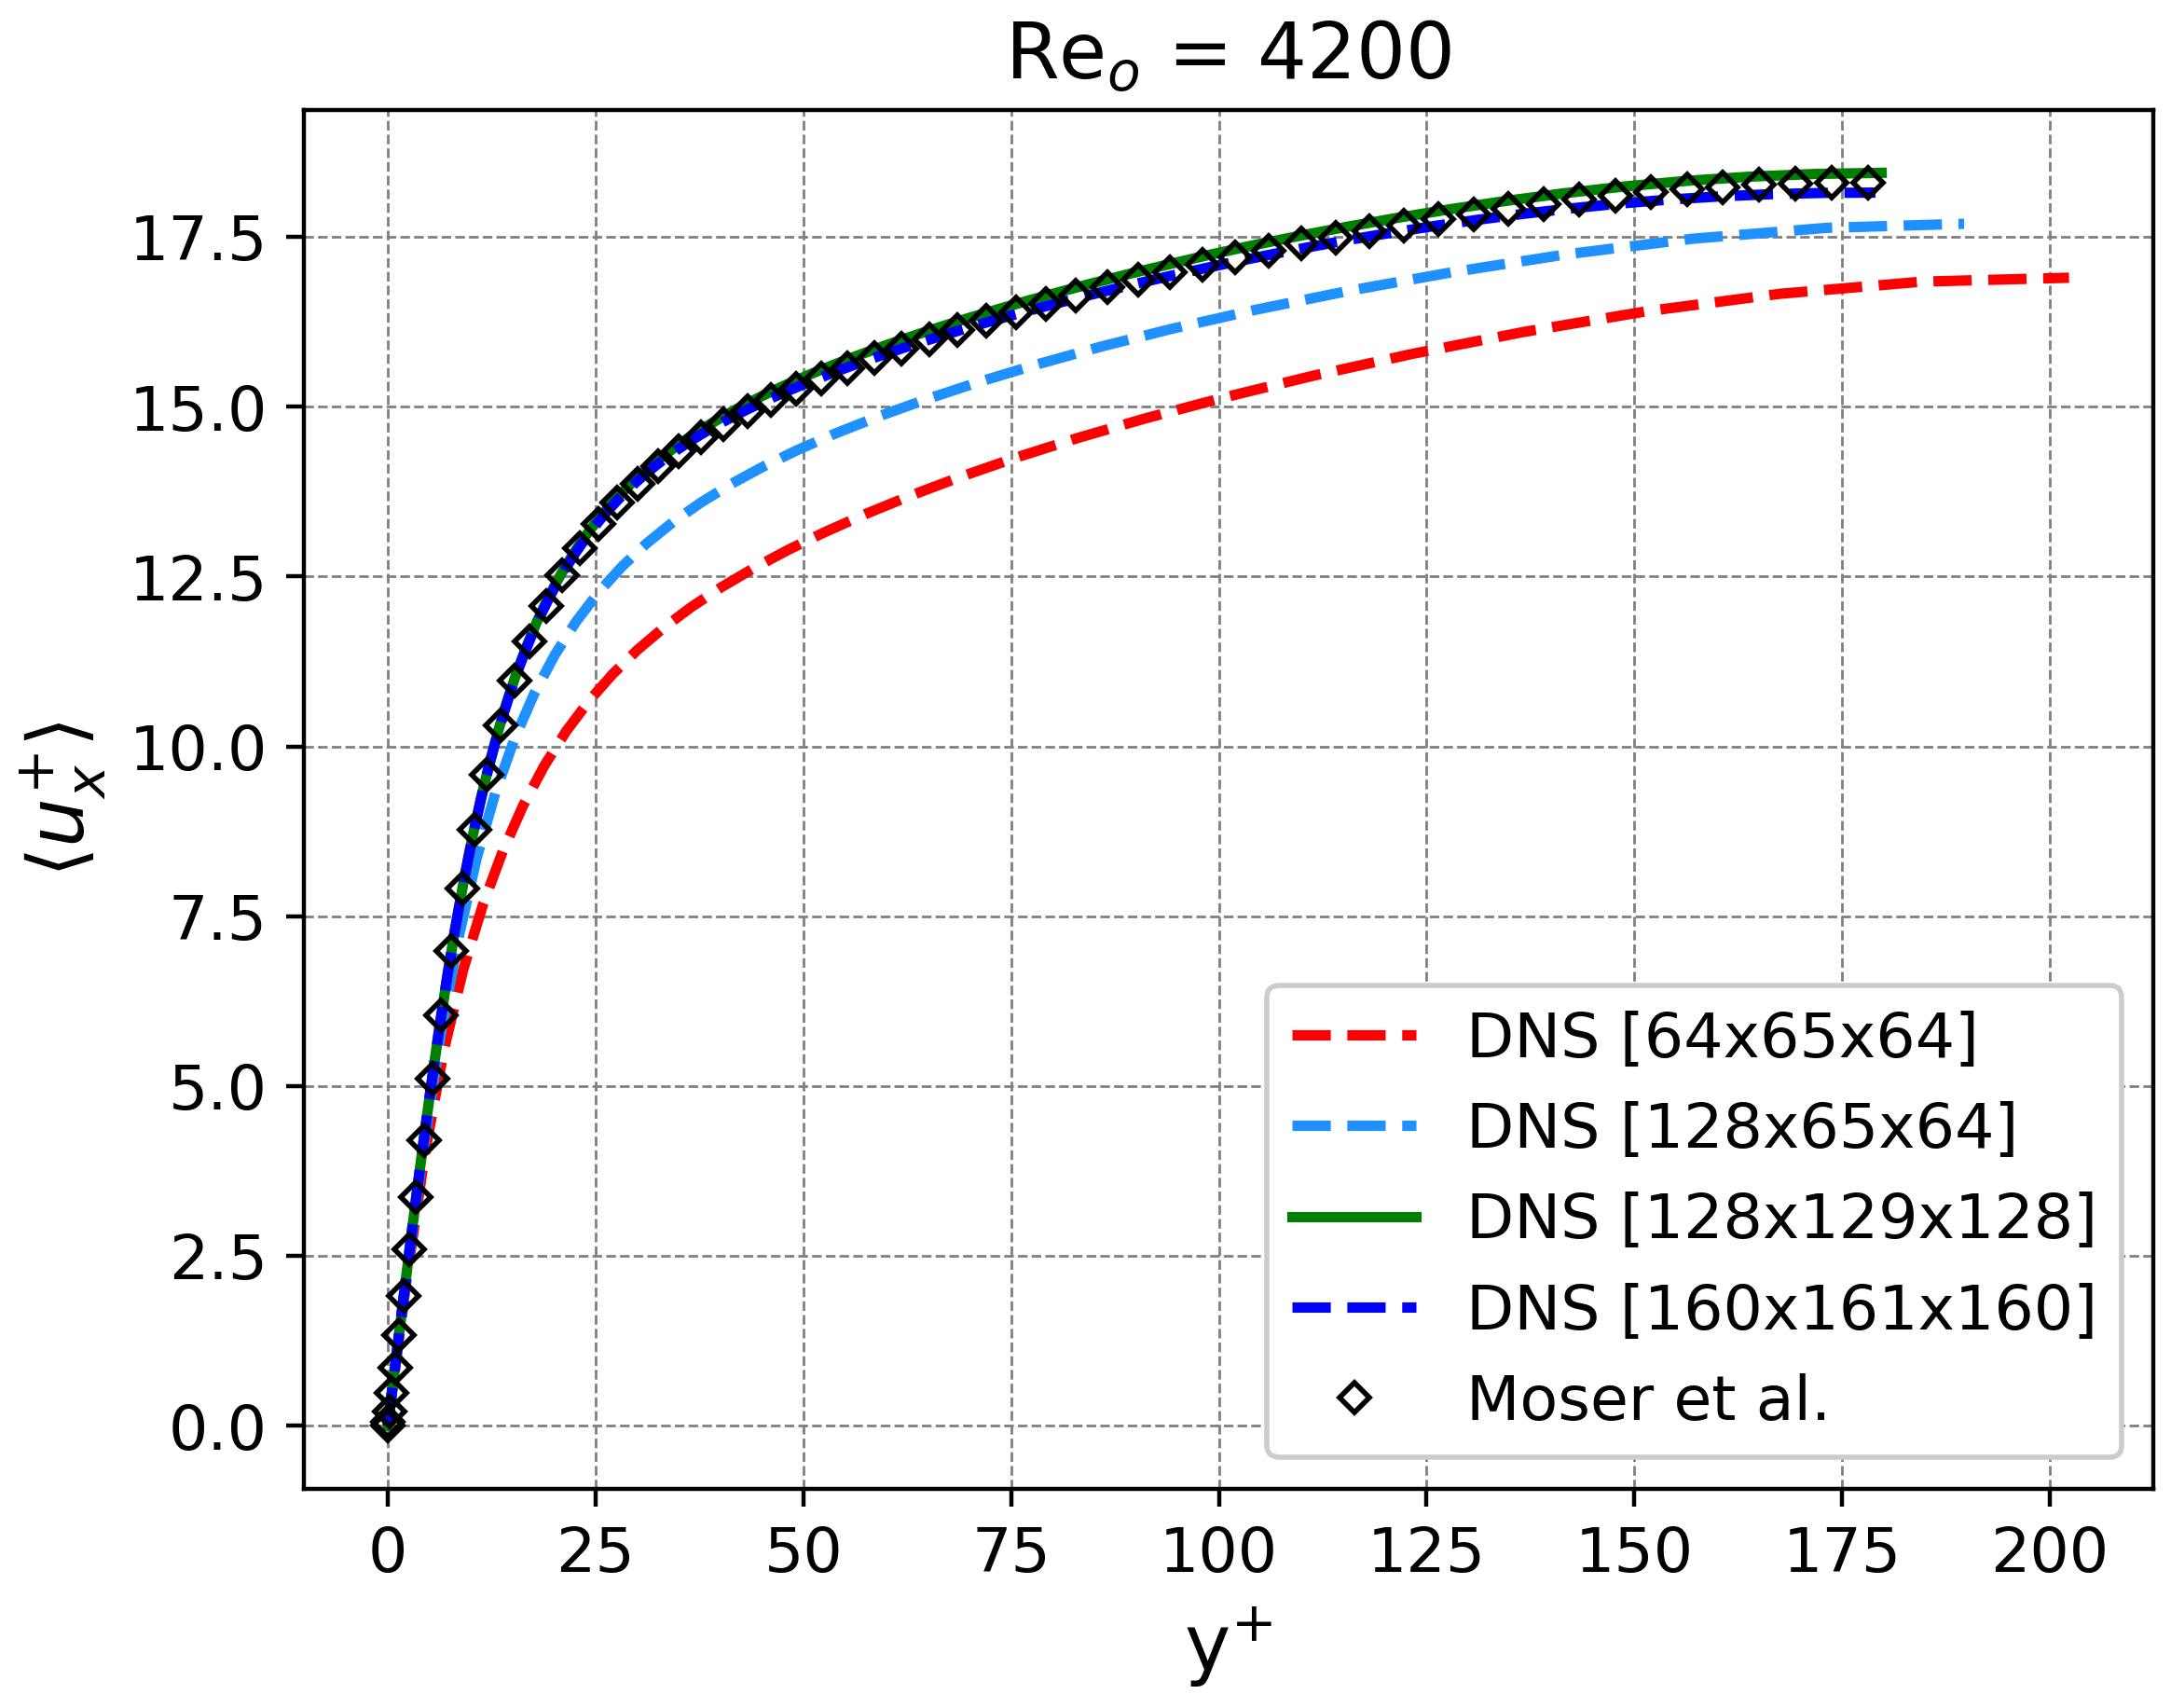
\includegraphics[width=0.49\textwidth]{figures/cap4/kim/ux_mean.png}
    	\label{fig:kim-ux}}  
    \subfloat[]{
    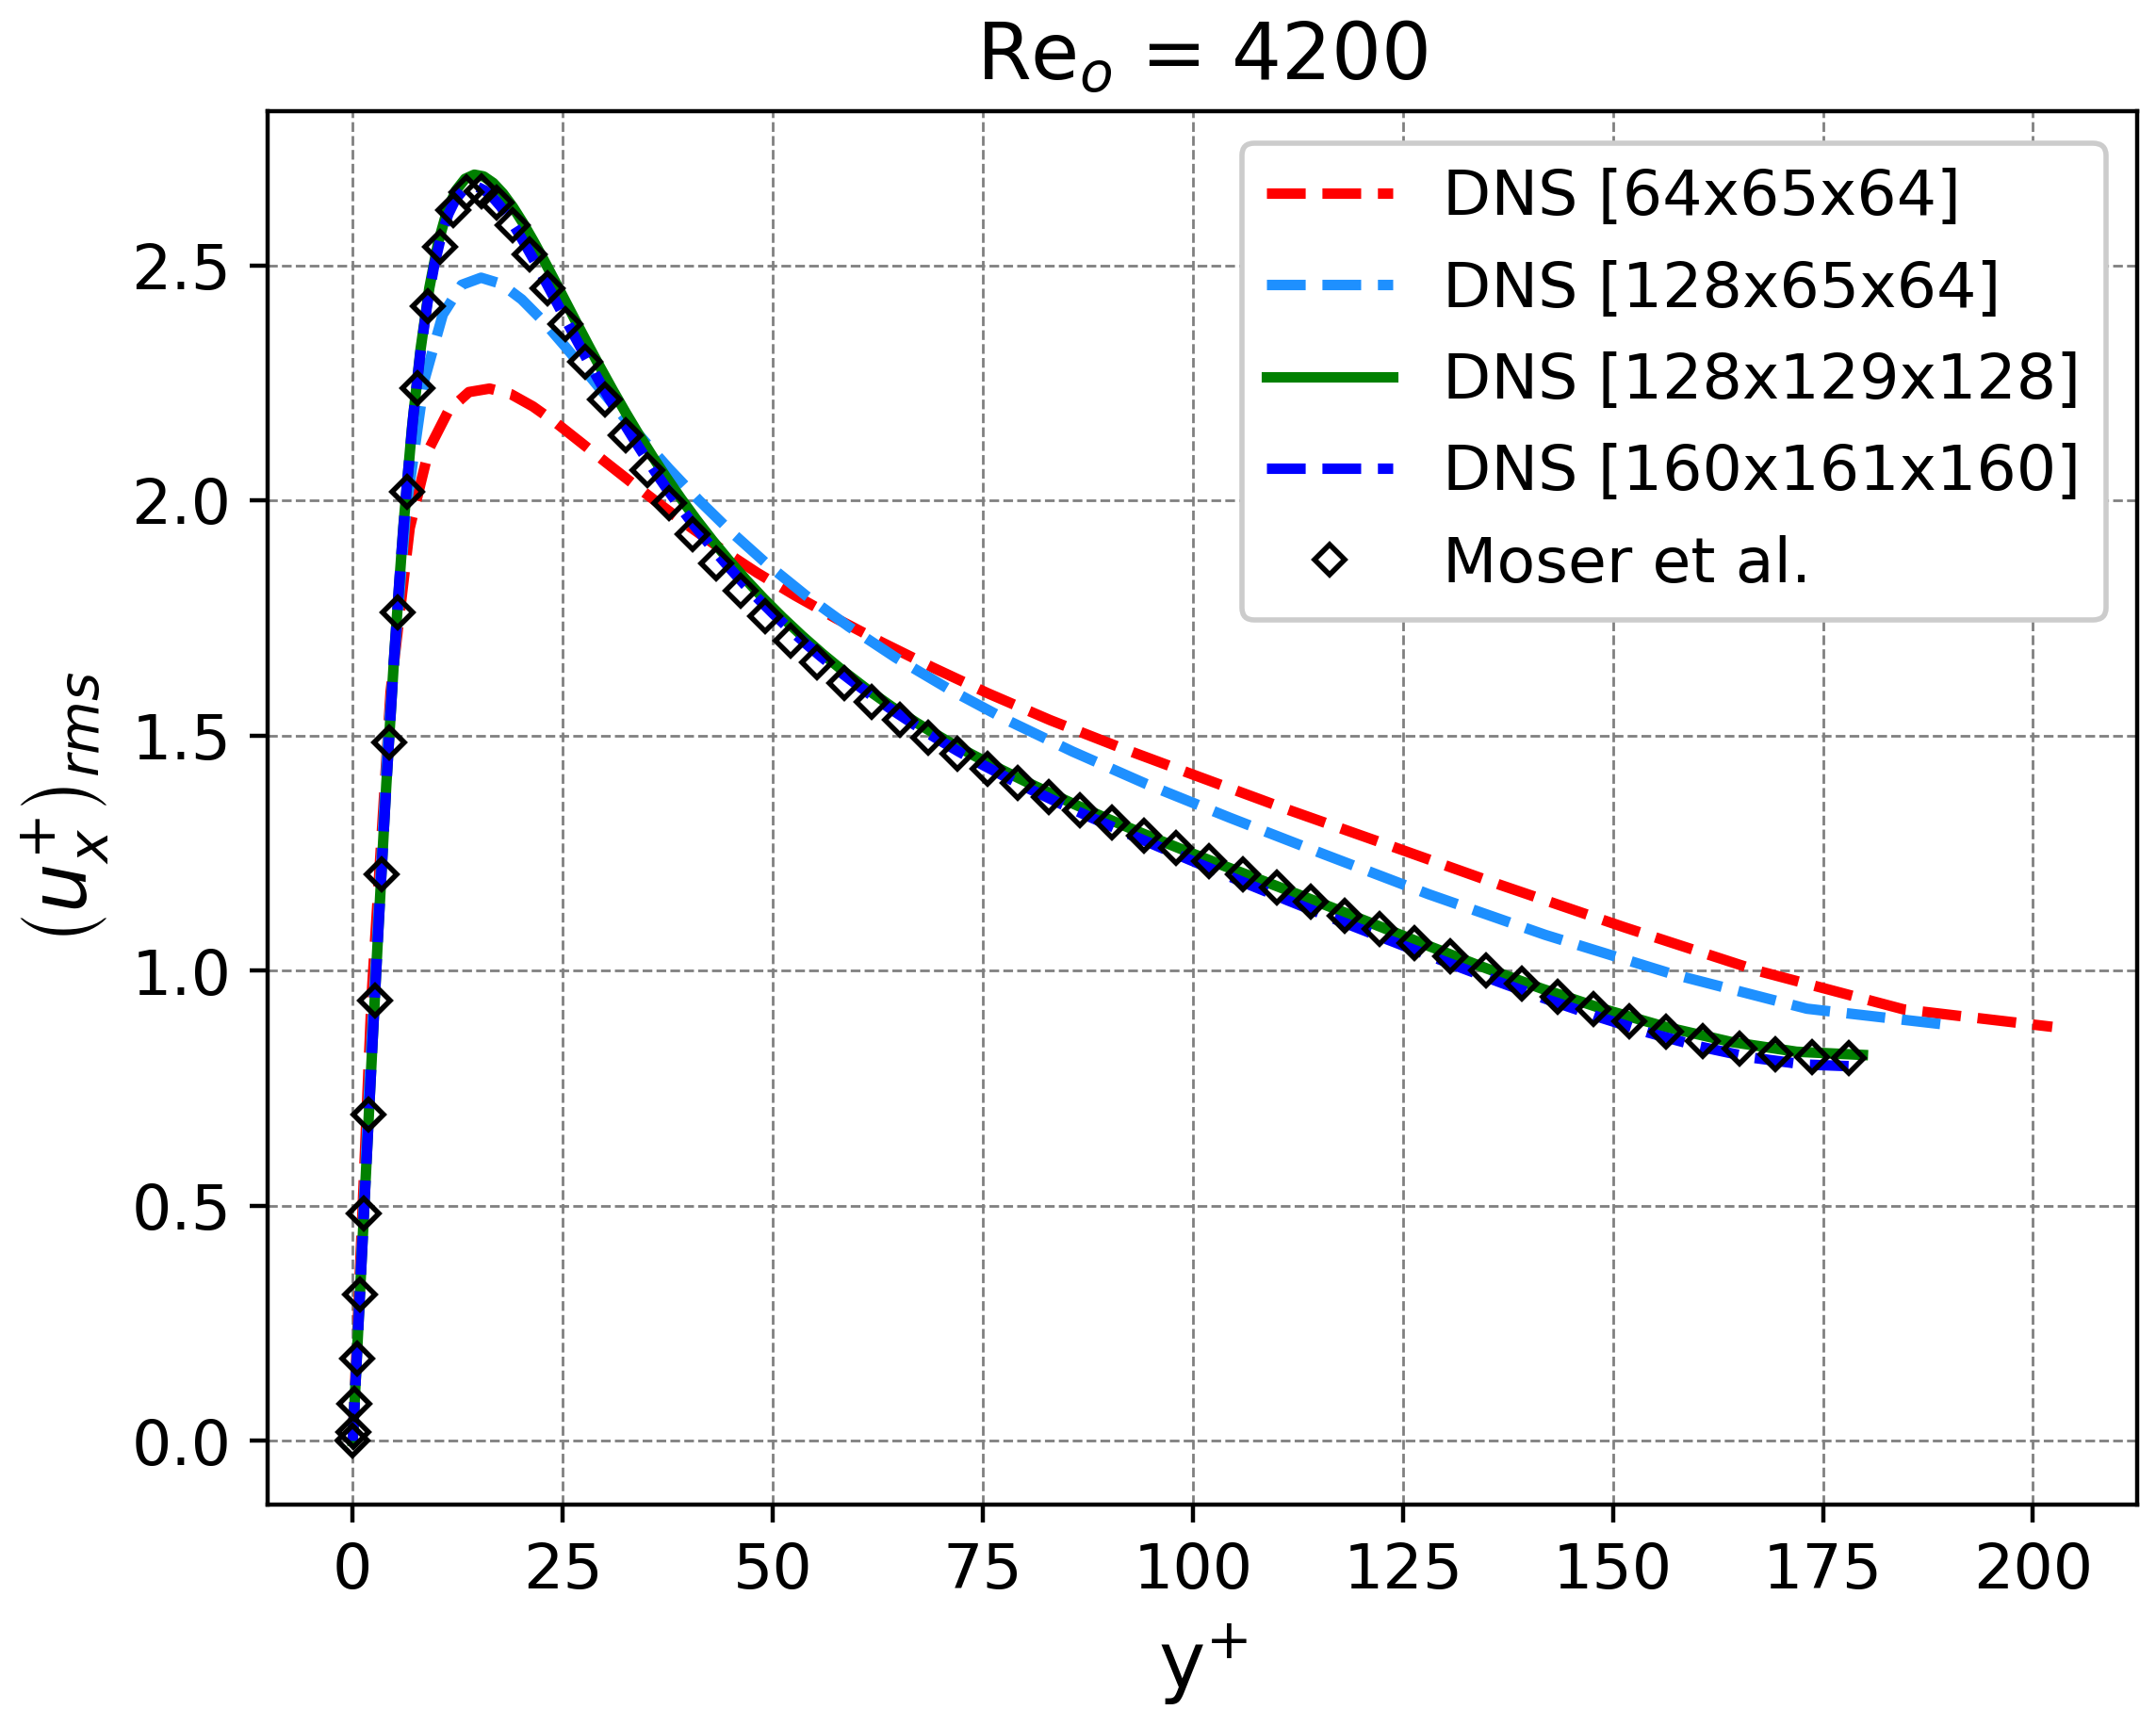
\includegraphics[width=0.49\textwidth]{figures/cap4/kim/ux_rms.png}
    	\label{fig:kim-ux-rms}}
    
    \subfloat[]{
    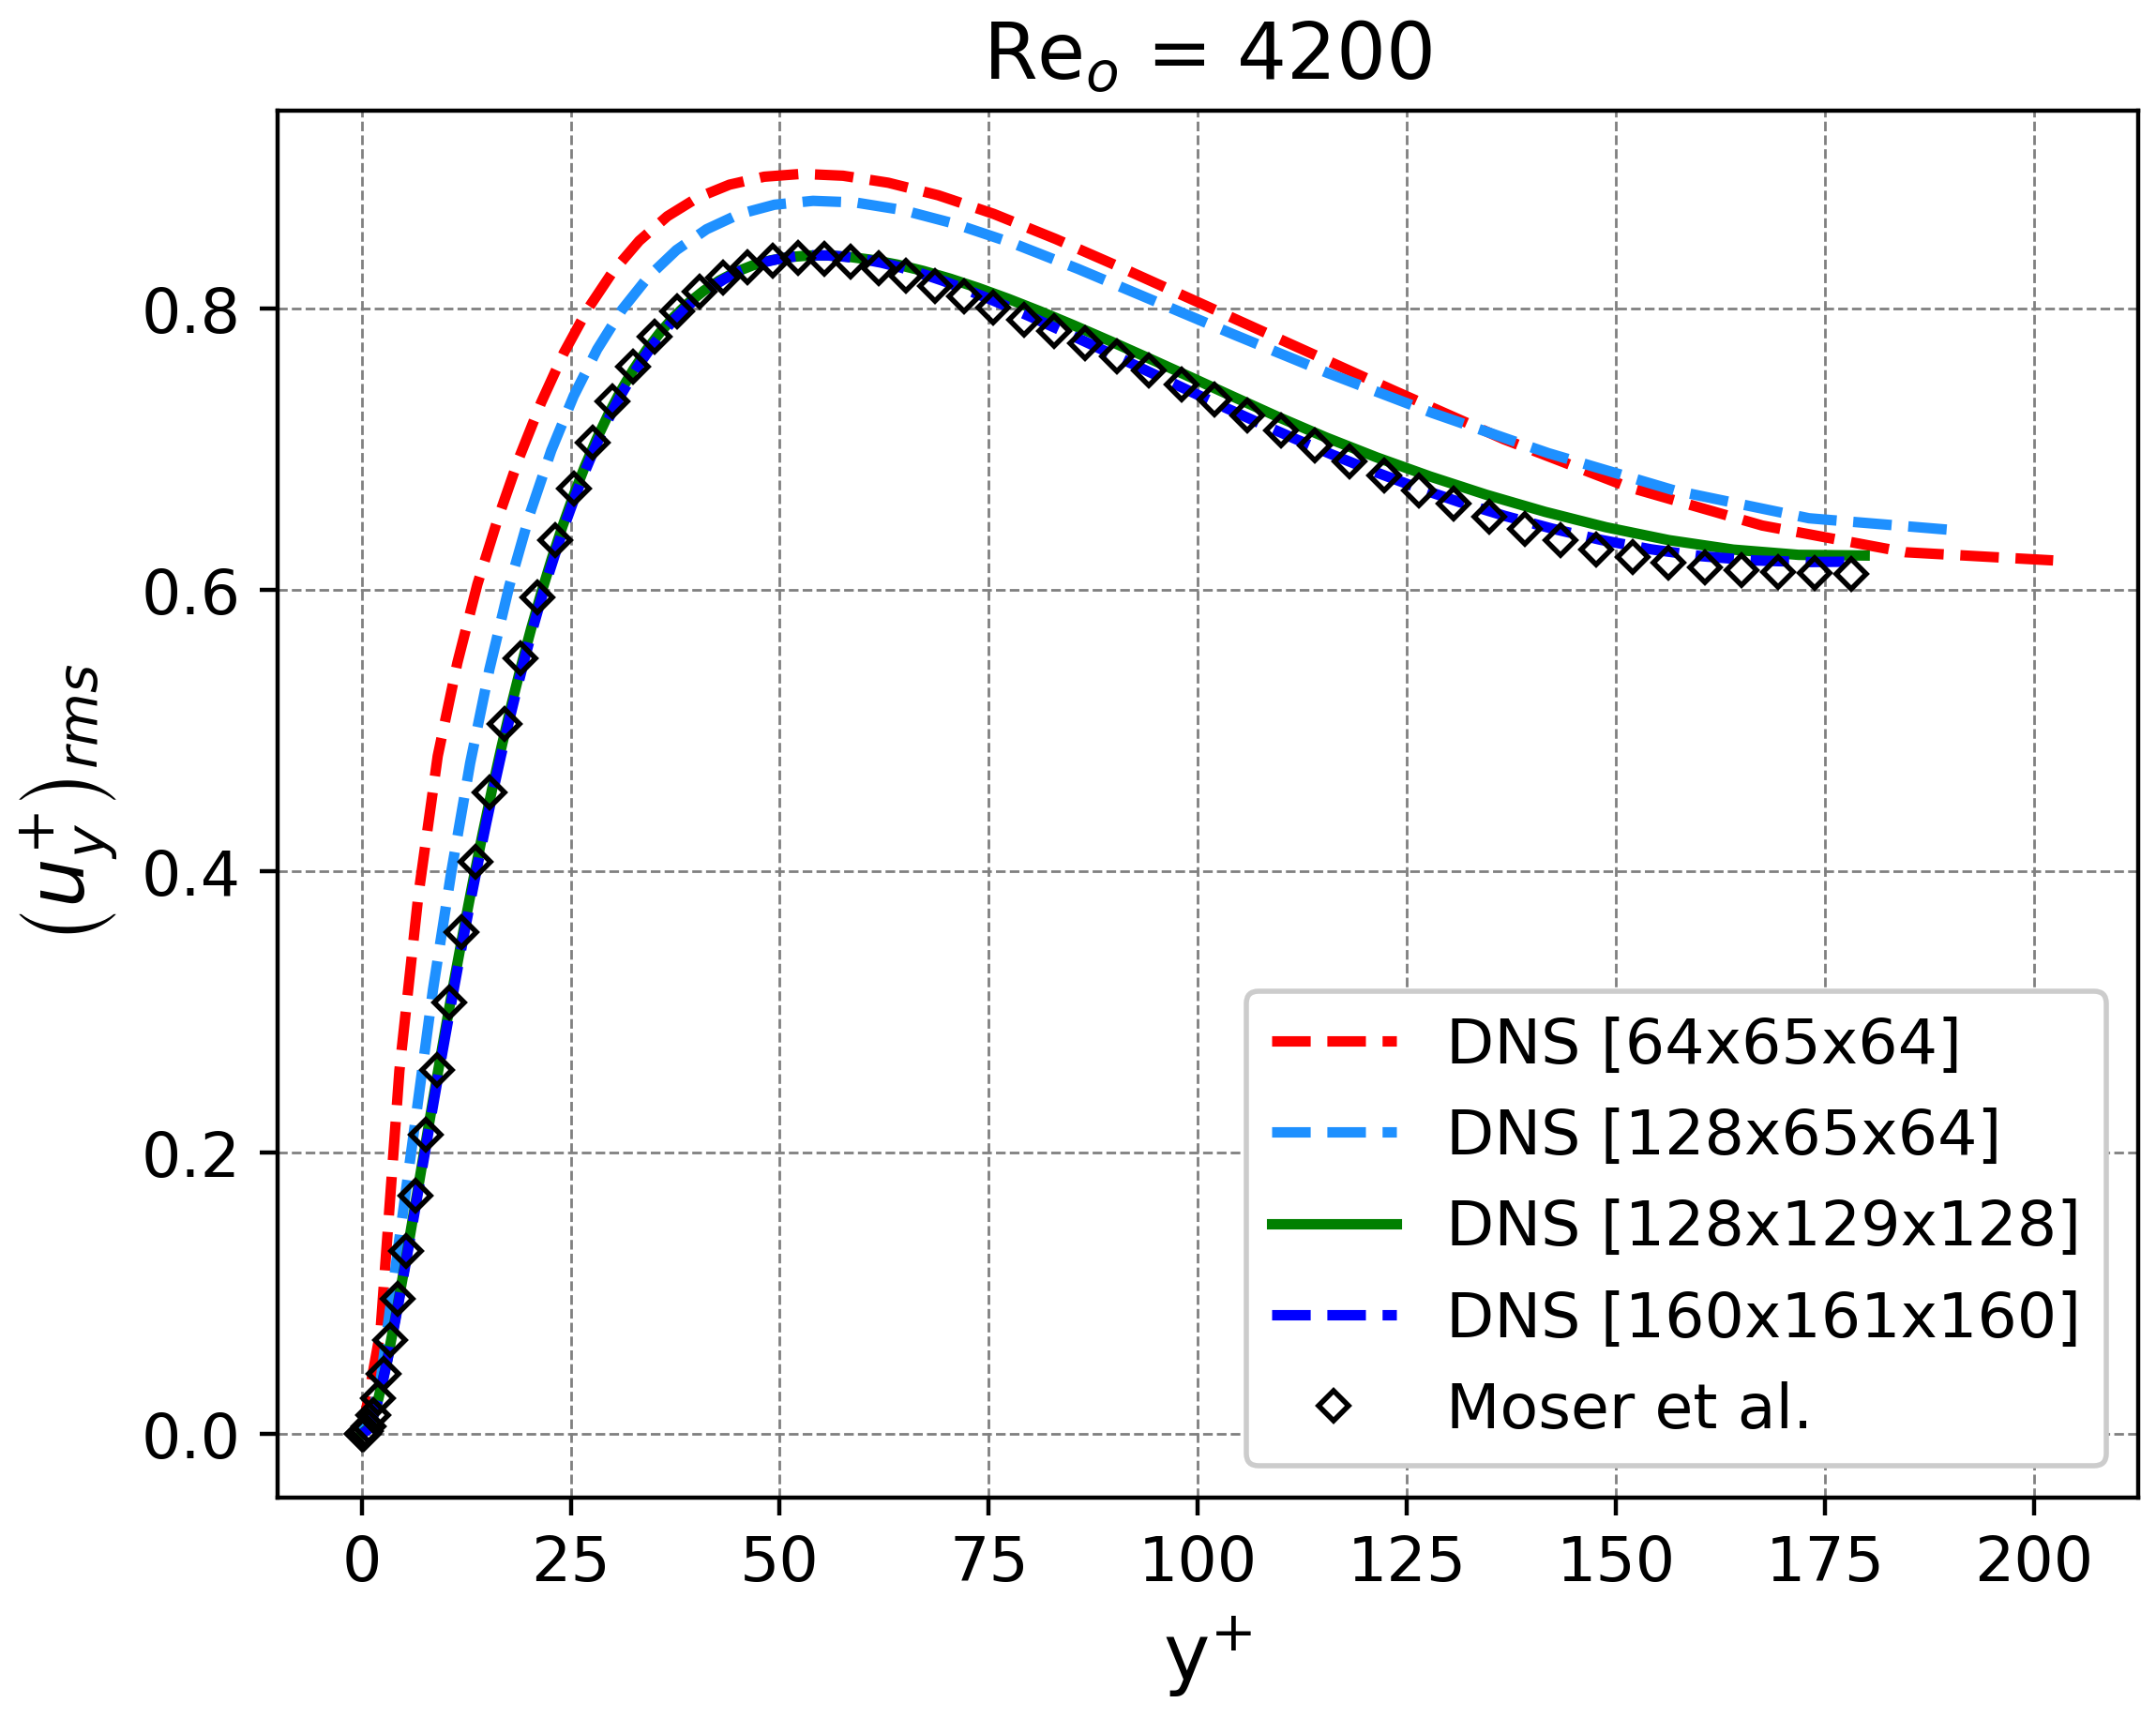
\includegraphics[width=0.49\textwidth]{figures/cap4/kim/uy_rms.png}
    	\label{fig:kim-uy}}  
    \subfloat[]{
    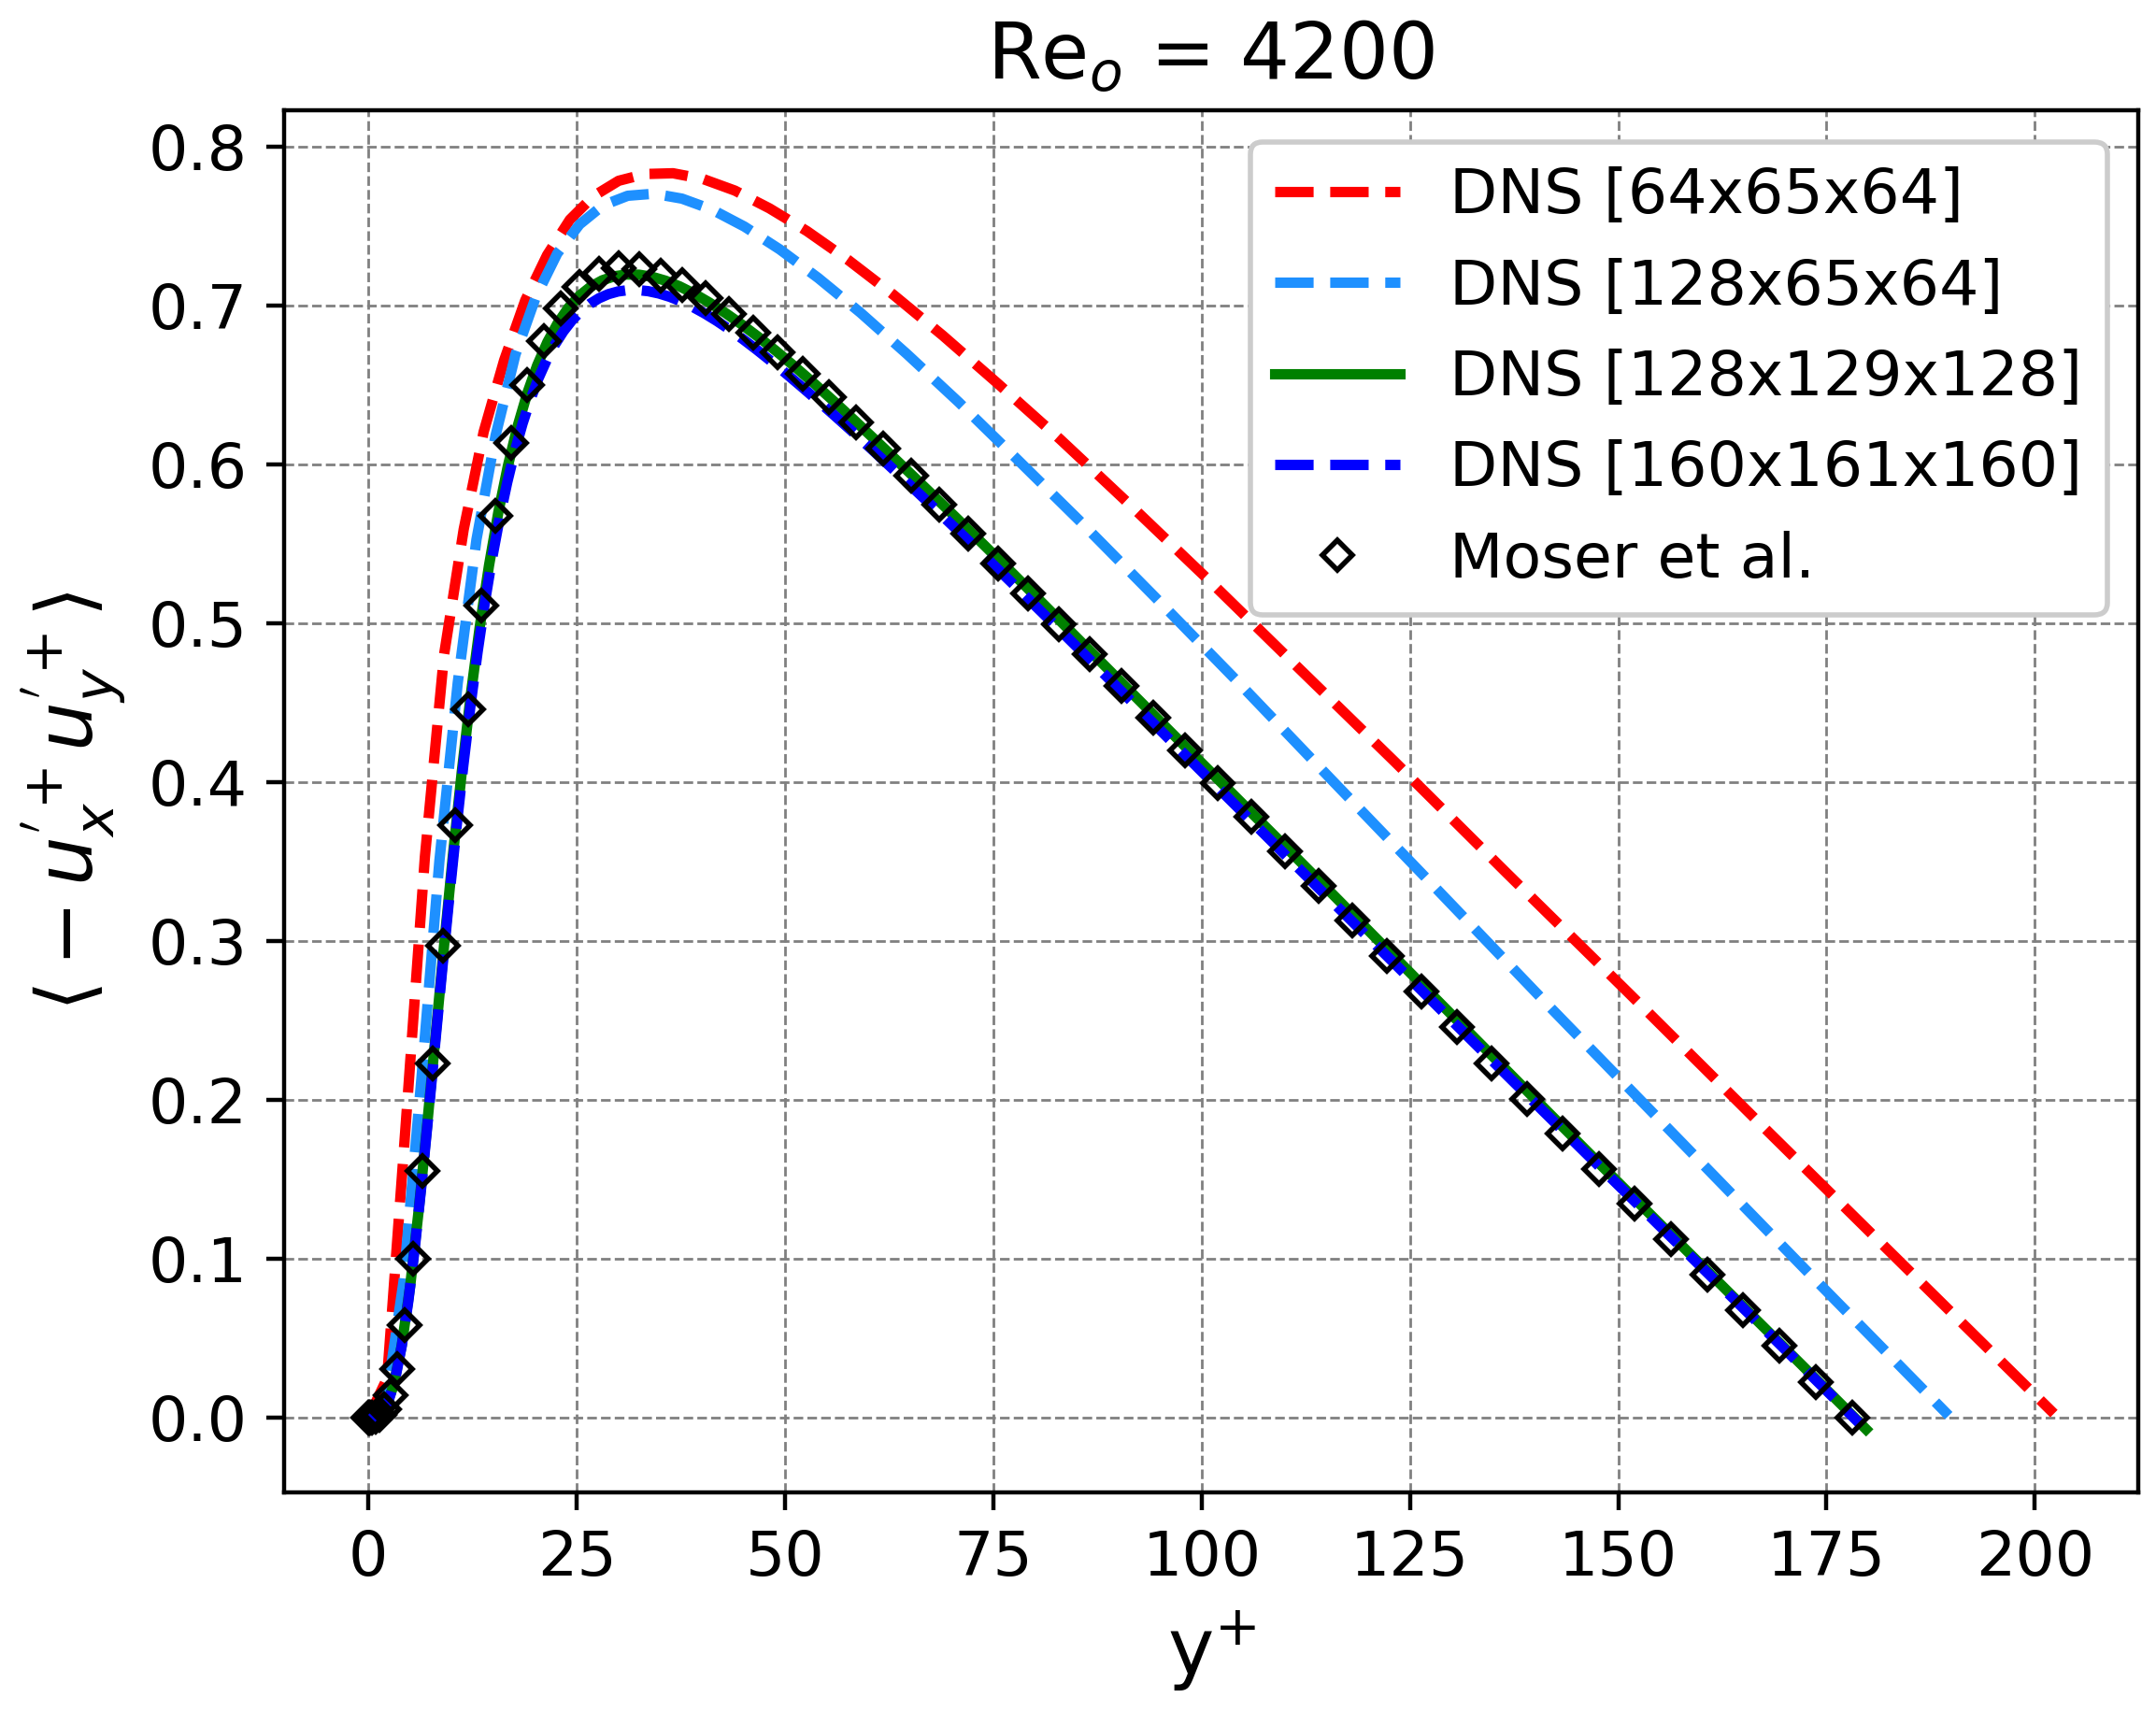
\includegraphics[width=0.49\textwidth]{figures/cap4/kim/up_vp.png}
    	\label{fig:kim-uxuy}} 
 \caption{Perfiles de \textbf{(a)} velocidad media \textit{streamwise}, \textbf{(b)} fluctuaciones RMS de la velocidad en $\langle u^+_x \rangle$, \textbf{(c)} fluctuaciones RMS de la velocidad $\langle u^+_y \rangle$ y \textbf{(d)} componente $xy$ del tensor de Reynolds. } 
 \label{fig:kim_1}
\end{figure}

\begin{table}[H]
\centering
\resizebox{0.9\textwidth}{!}{%
\begin{tabular}{lccccc}
\toprule
Nomenclatura & L$_x \times$ L$_y \times$ L$_z$ & N$_x \times$ N$_y \times$ N$_z$ & $(\Delta x^*,\Delta z^*)$ & $\Delta y^*_{\text{max}}$ \\
\midrule
A & $6\text{.}4d \times 2 \times 3\text{.}2d $ & $128 \times 66 \times 128$    & (0.05, 0.025) & 0.064 \\
C & $12\text{.}8d \times 2 \times 6\text{.}4d $ & $256 \times 128 \times 256$  & (0.05, 0.025) & 0.033 \\
D & $6\text{.}4d \times 2 \times 3\text{.}2d $ & $1024 \times 480 \times 512$   & (0.006, 0.006) & 0.0054 \\

\bottomrule
\end{tabular}}
\caption{Resoluciones espaciales empleadas por Kawamura \textit{et al.} \cite{kawamura2000dns}.}
\label{tab:meshes-kawa}
\end{table}

\newpage


\subsection{Situación II. Transporte de escalar pasivo en convección forzada con $q''_w$ constante}

En este caso se considera sólo el régimen de convección forzada, lo que equivale a suponer $\Pi=0$ en la ecuación de momento. De esta forma, las ecuaciones de continuidad y momento quedan desacopladas de la ecuación de energía (ecuaciones \ref{eq:gob_system_adim}). En este sentido, los campos solución de la velocidad son exactamente los mismos que en la \textbf{Situación I} y el campo de temperatura es un campo escalar que no interviene en el desarrollo hidrodinámico del sistema, sino únicamente en el aspecto térmico del flujo. Por ello, sólo se presentan magnitudes asociadas a la temperatura adimensional. Para las simulaciones asociadas a esta subsección, se considera el número de Reynolds Re$_o=4278$. 

\paragraph{Convergencia en Malla.}
En primer lugar, se analiza la respuesta del campo escalar solución frente a diferentes mallas, en concreto, se emplean aquellas mismas utilizadas en la \textbf{Situación I}.  Las Figuras \ref{fig:kmesh-theta} - \ref{fig:kmesh-uy-theta} presentan los perfiles de la temperatura adimensional, sus fluctuaciones y los flujos de calor turbulento en las direcciones X e Y, respectivamente. Las \linebreak simulaciones propias se comparan con aquellas obtenidas en la referencia \cite{kawamura2000dns} para Pr=0.71. Además, en dichas gráficas se exponen los distintos resultados obtenidos por Kawamura \textit{et al.} para diferentes mallas empleadas en su trabajo (véase Tabla \ref{tab:meshes-kawa}). 




De forma análoga al caso anterior, se observa claramente la convergencia con el refinamiento de malla: a medida que aumenta la resolución, los resultados se mantienen en buen acuerdo con las referencias. En particular, las curvas correspondientes a M2 y M3 no muestran diferencias apreciables a la escala de las figuras; en otras palabras, el paso de M2 a M3 no introduce mejoras perceptibles. En este sentido, se observa que la malla M2 (un compromiso adecuado entre precisión y costo computacional) reproduce con buen acuerdo los resultados de Moser \textit{et al.} \cite{moser1999} y Kawamura \textit{et al.} \cite{kawamura2000dns}.

\newpage

\begin{figure}[H]
 \centering
    \subfloat[]{
    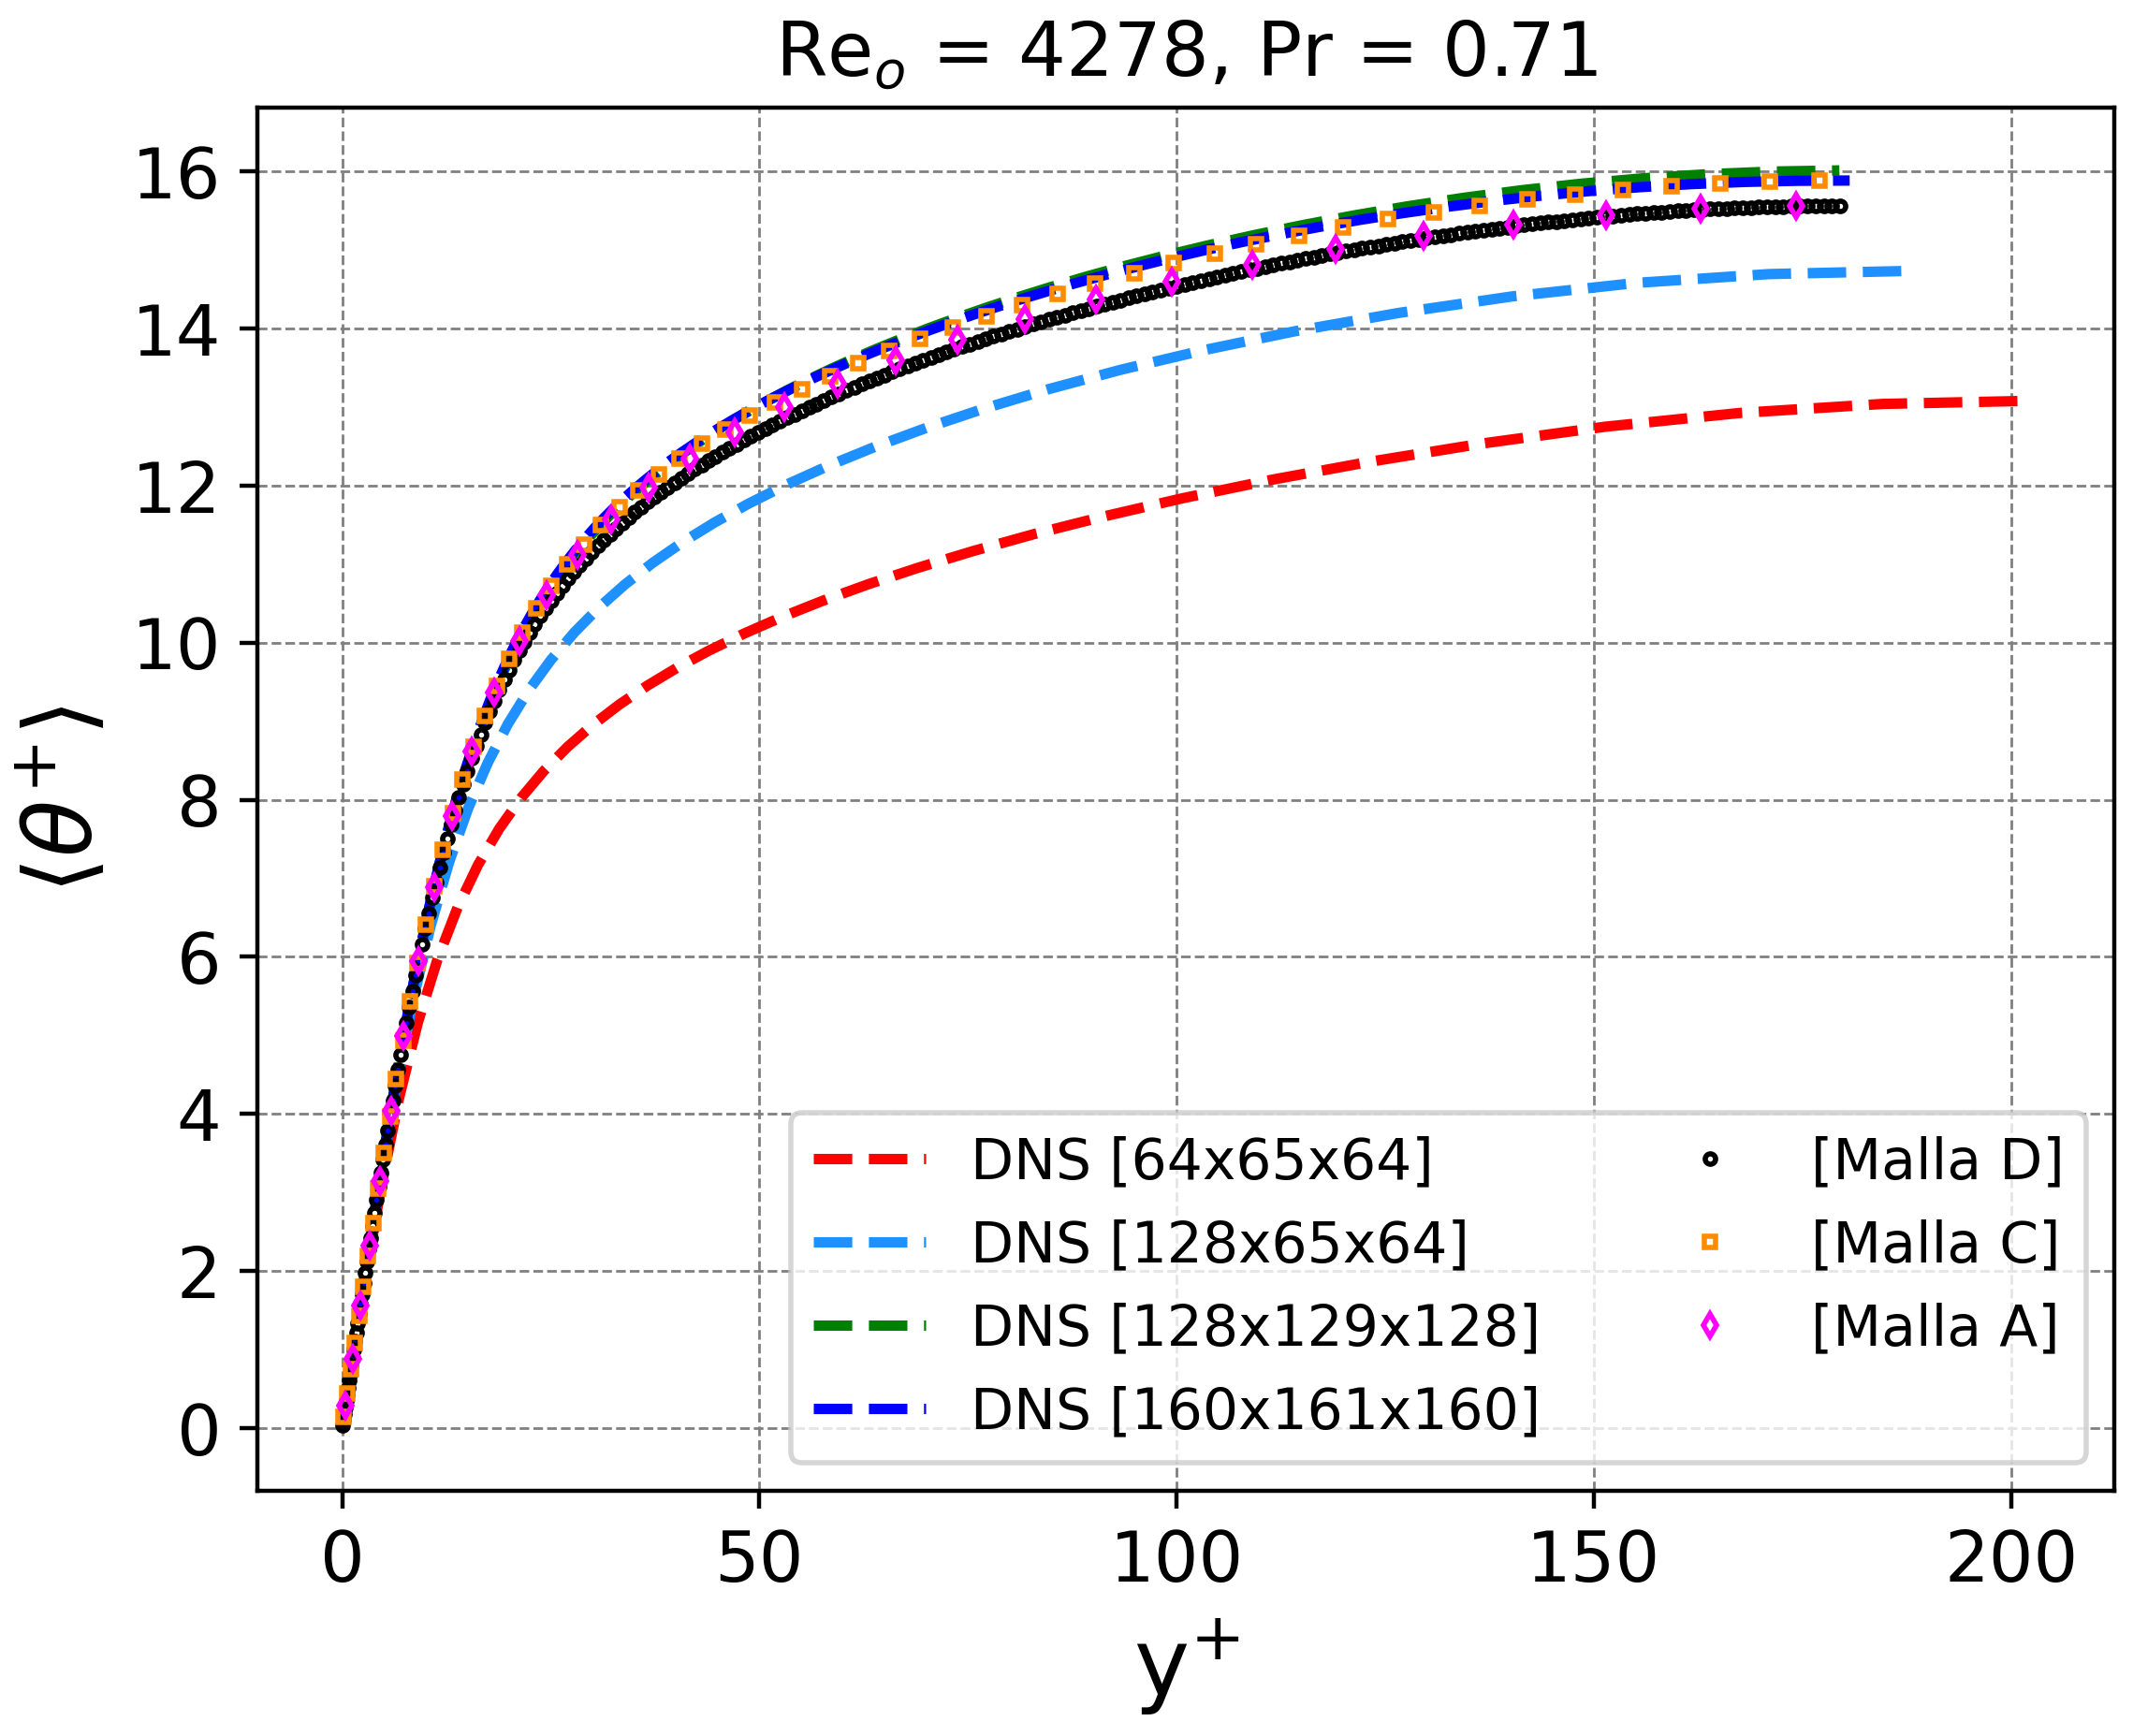
\includegraphics[width=0.49\textwidth]{figures/cap4/kawamura_mesh/tep_theta.png}
    	\label{fig:kmesh-theta}}  
    \subfloat[]{
    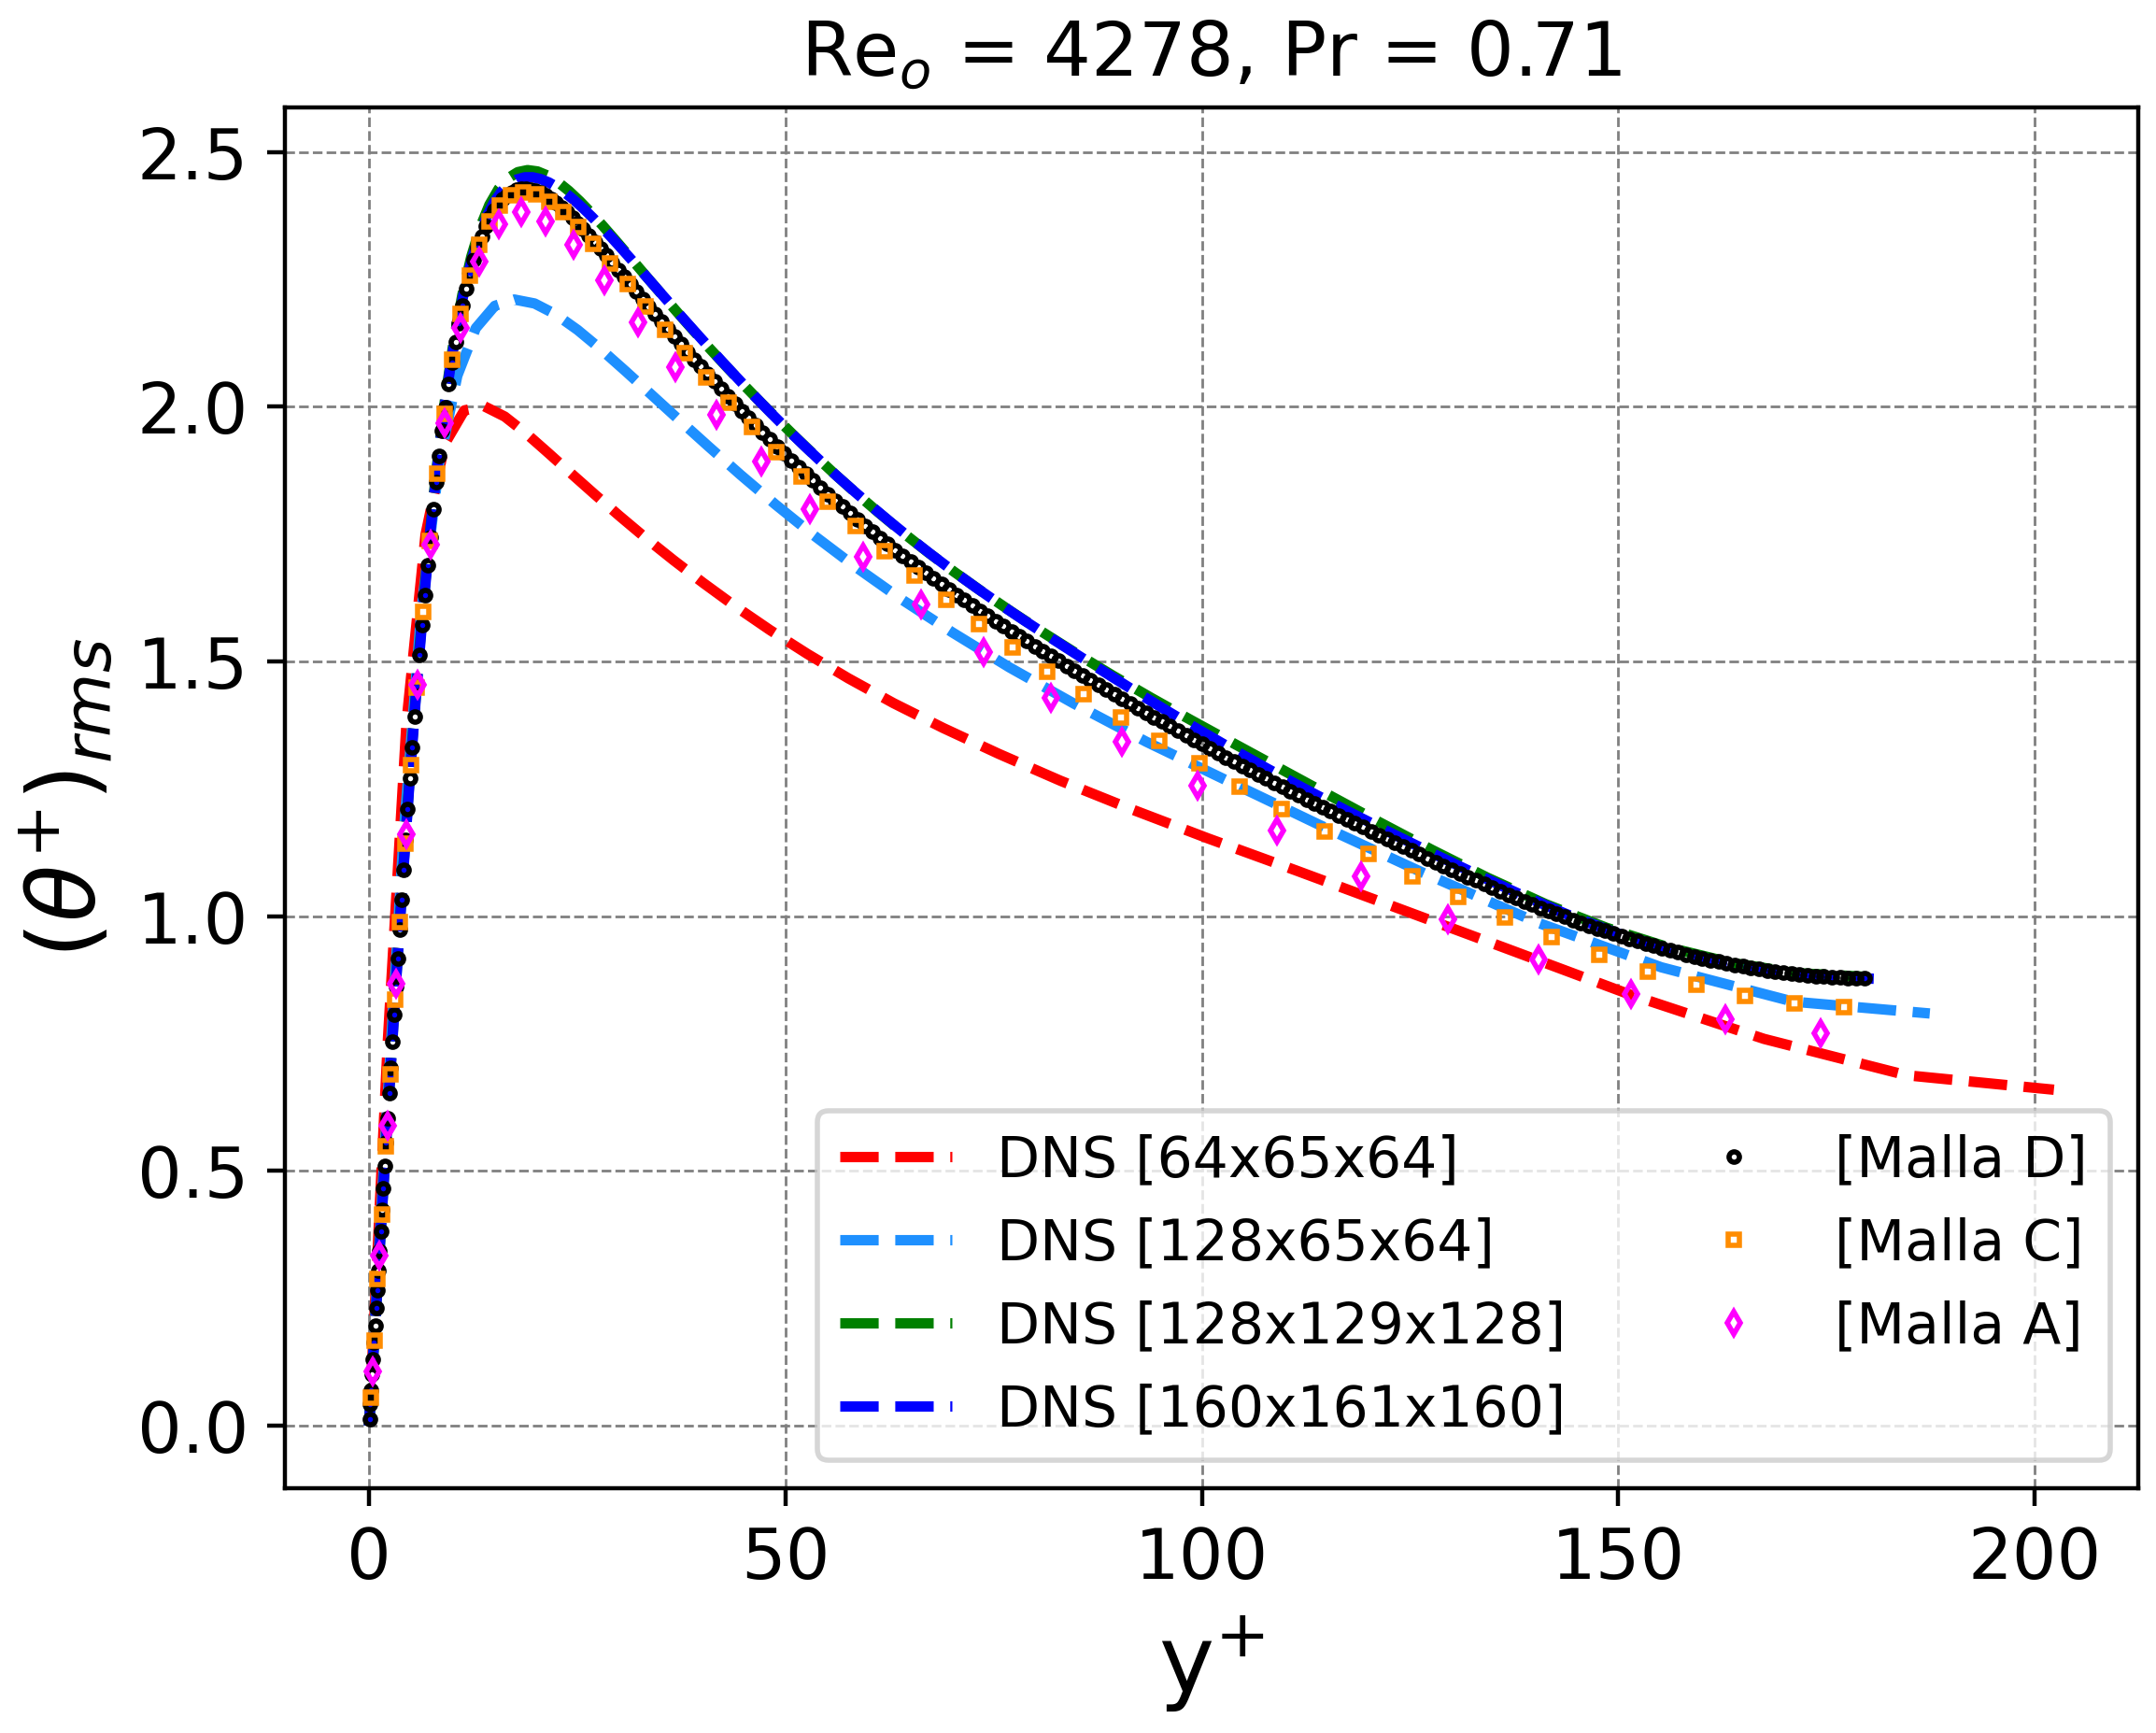
\includegraphics[width=0.49\textwidth]{figures/cap4/kawamura_mesh/tep_thetap_rms.png}
    	\label{fig:kmesh-theta-rms}}  

    \subfloat[]{
    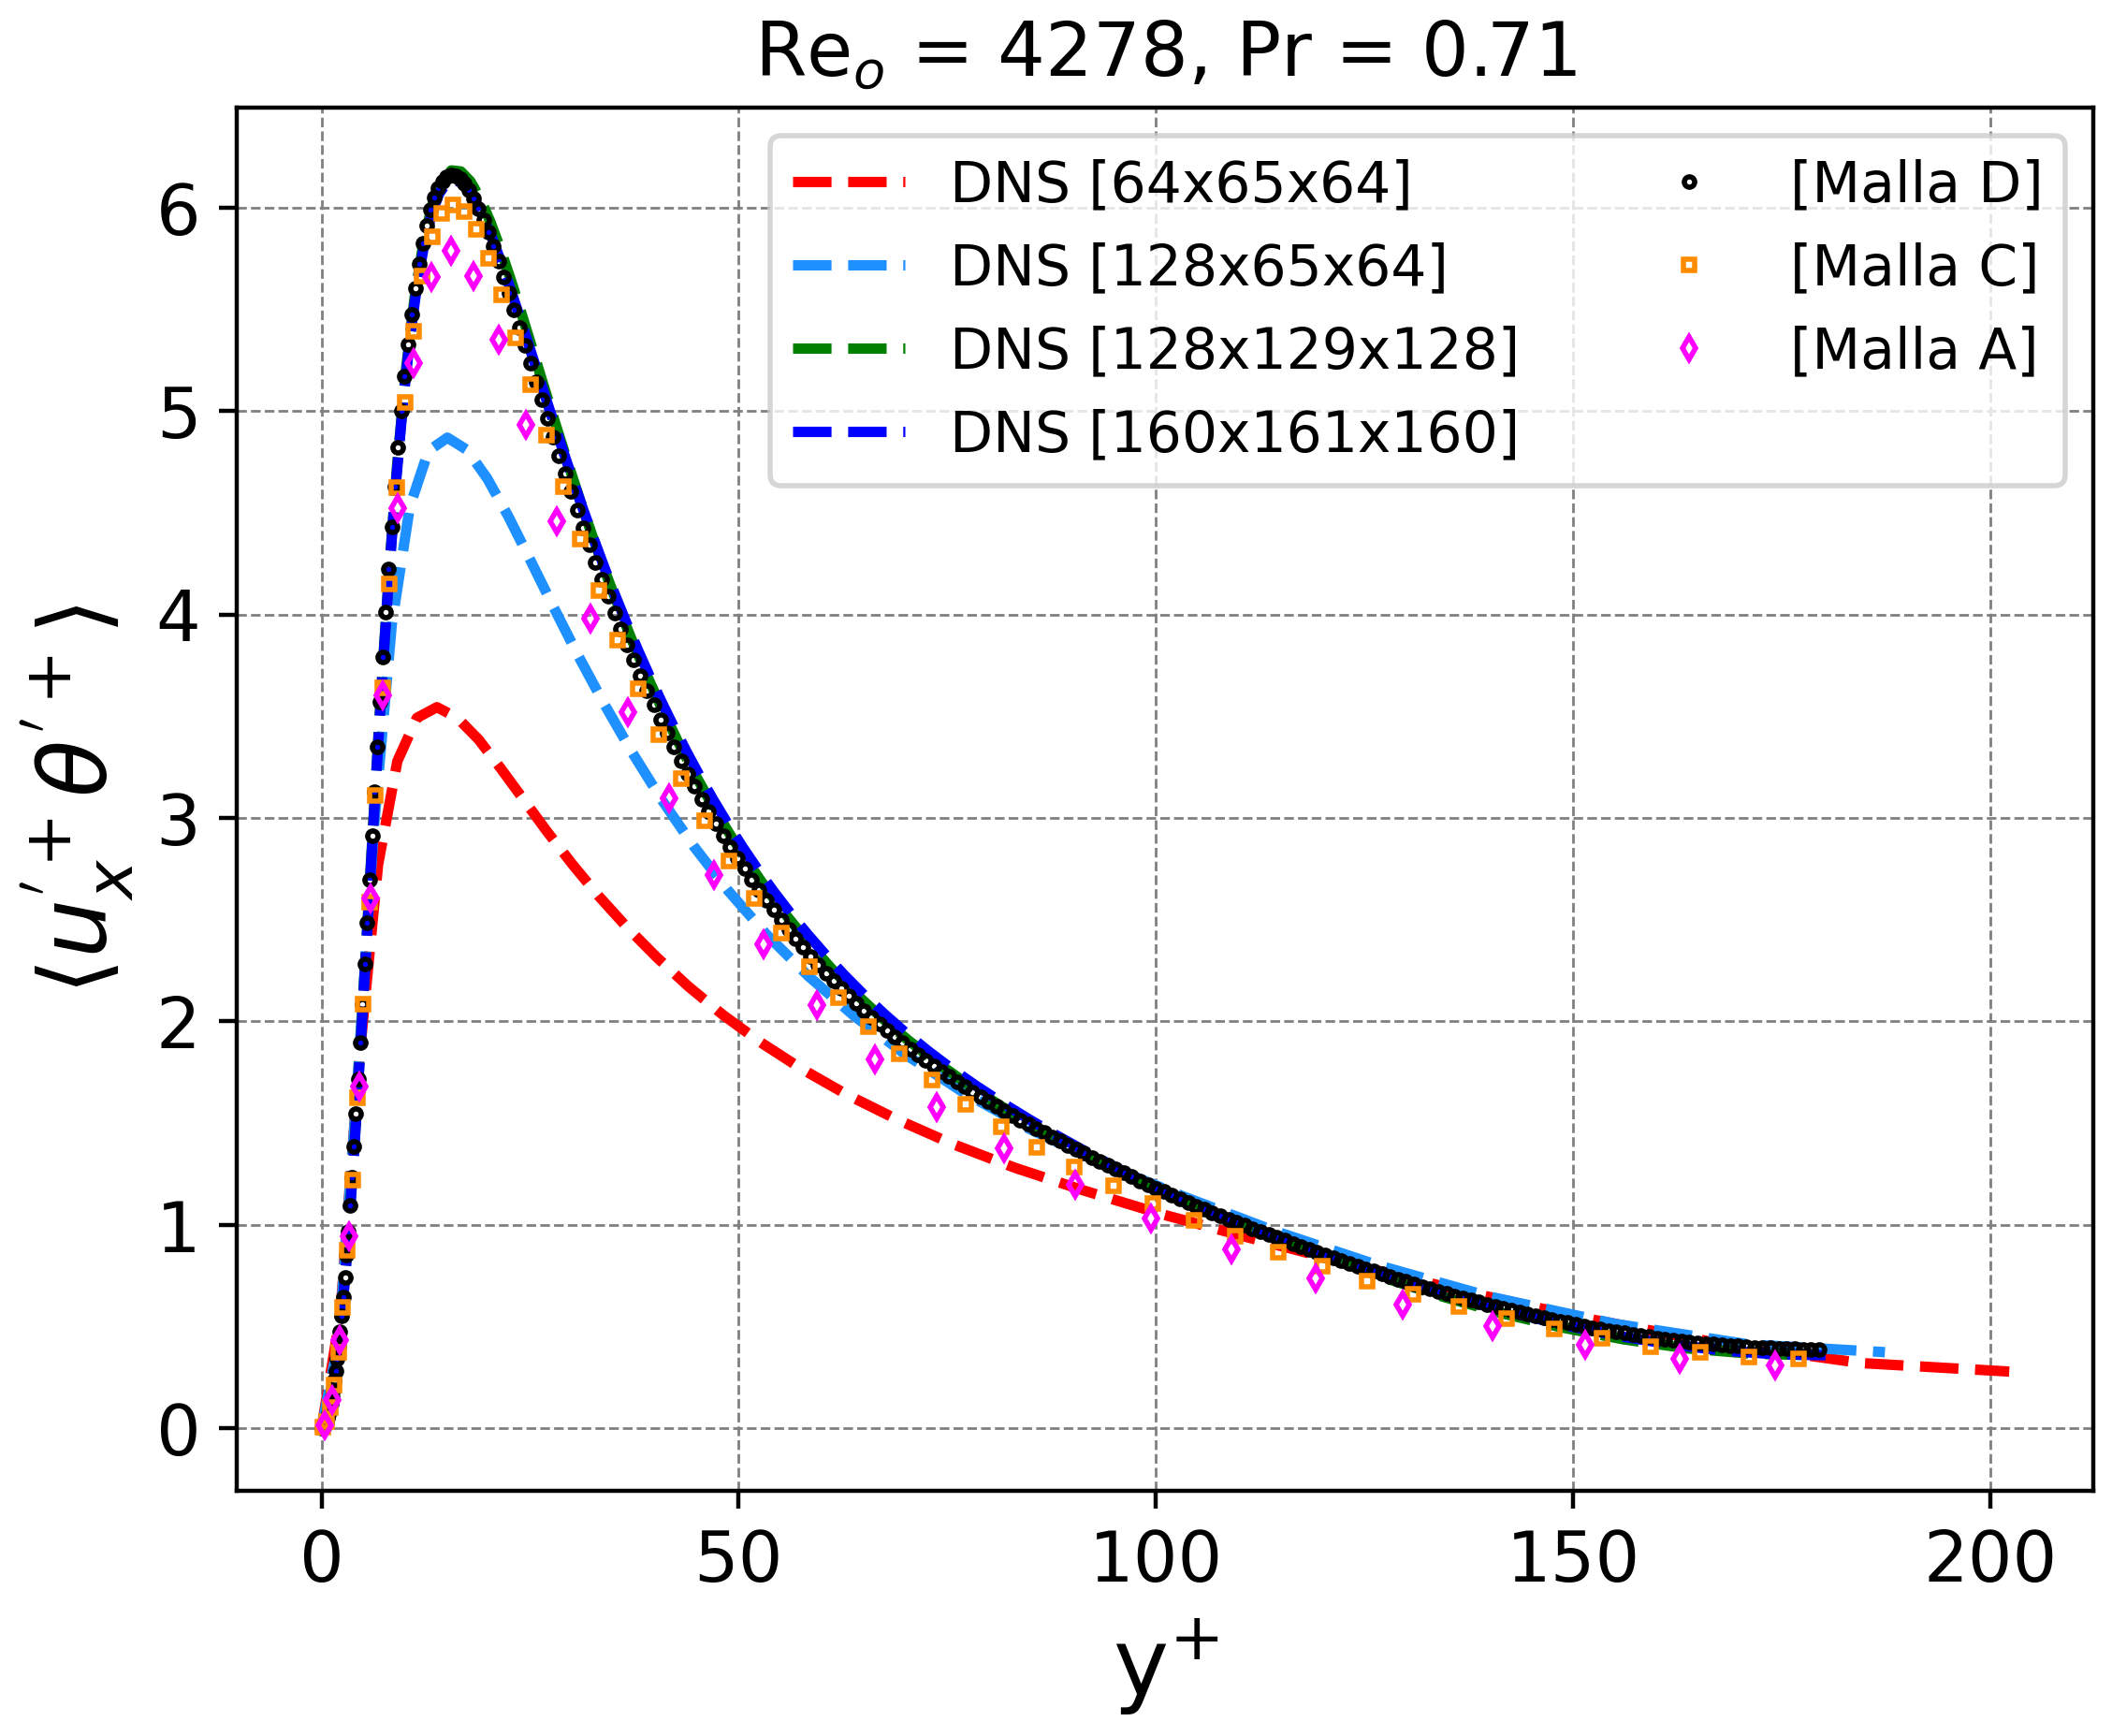
\includegraphics[width=0.49\textwidth]{figures/cap4/kawamura_mesh/tep_up_thetap.png}
    	\label{fig:kmesh-ux-theta}}  
    \subfloat[]{
    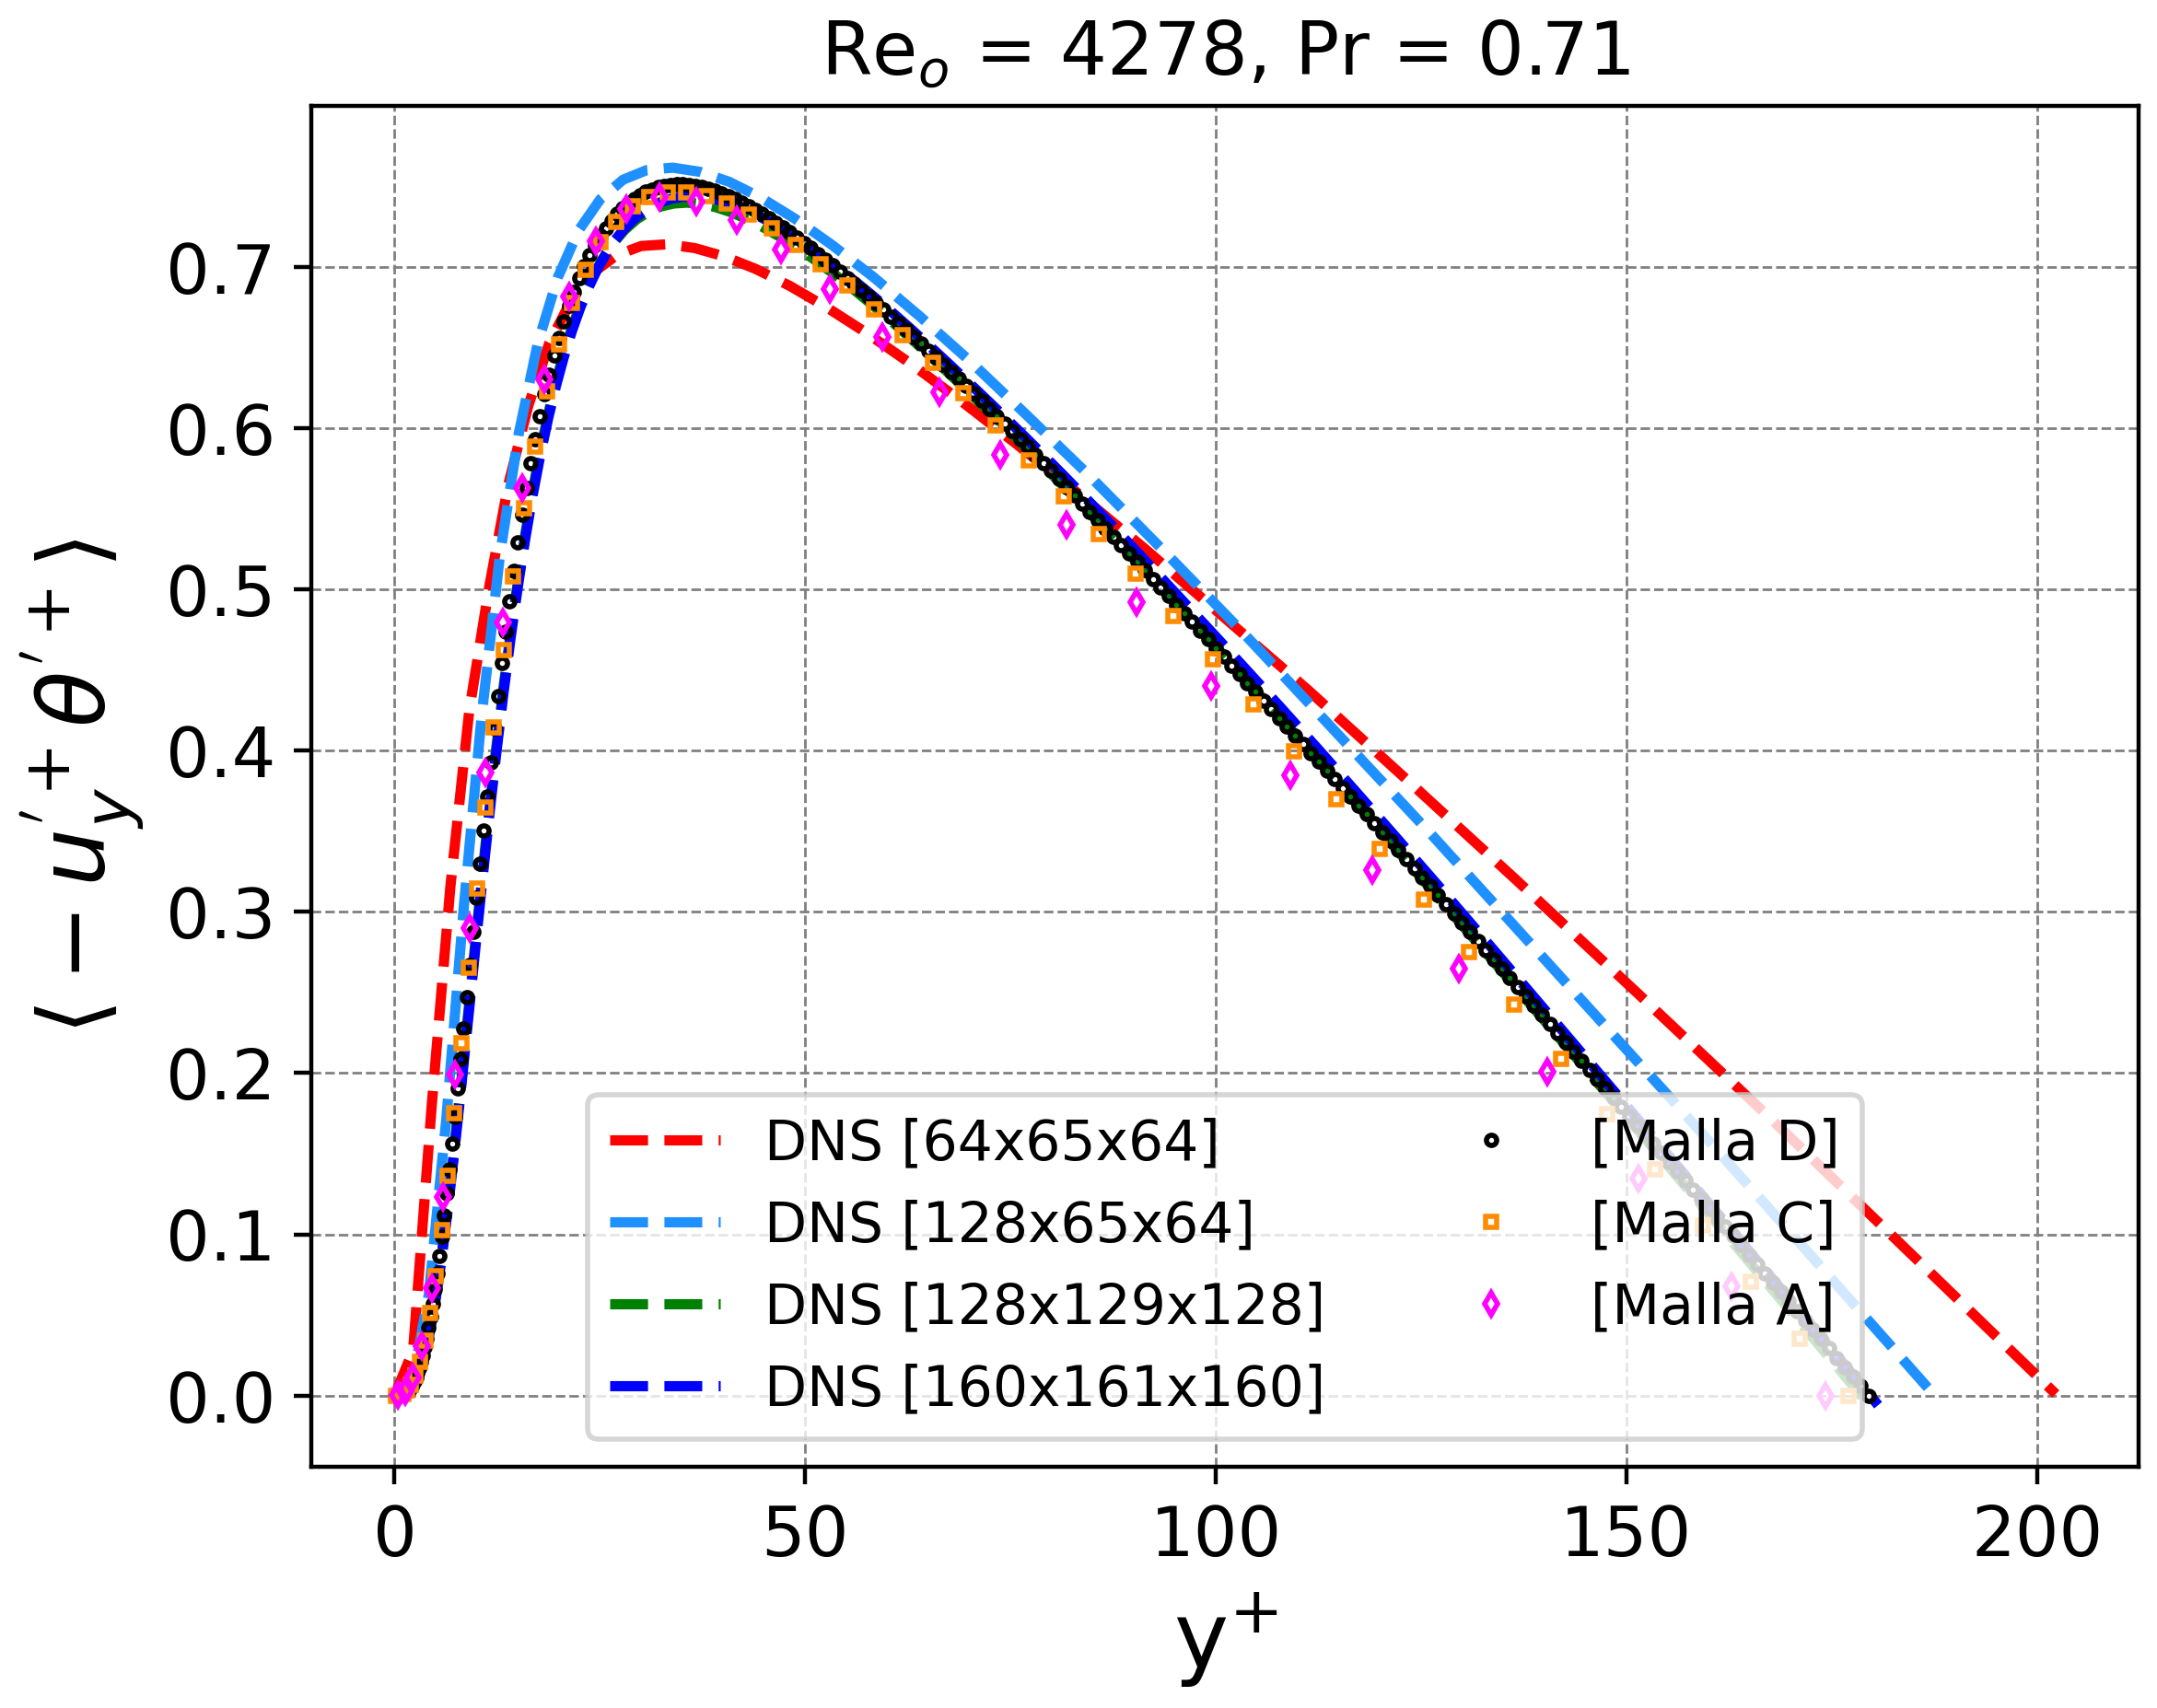
\includegraphics[width=0.49\textwidth]{figures/cap4/kawamura_mesh/tep_vp_thetap.png}
    	\label{fig:kmesh-uy-theta}}  
 \caption{Perfiles de \textbf{(a)} temperatura adimensional media, \textbf{(b)} fluctuaciones RMS de la temperatura adimensional, \textbf{(c)} flujo de calor turbulento en la dirección X, $\langle u^+_x \theta^+ \rangle$, y \textbf{(d)} flujo de calor turbulento en la dirección Y, $\langle u^+_y \theta^+ \rangle$.} 
 \label{fig:kmesh_1}
\end{figure}

\paragraph{Variación del número de Prandtl.}
La segunda parte consiste en emplear la malla M2 para distintos números de Prandtl, en particular, aquellos empleados en el trabajo de Kawamura \textit{et al.}: Pr= 0.025, 0.71, 1 y 7. De igual forma que para la convergencia en malla, en las Figuras \ref{fig:kpr-theta} - \ref{fig:kpr-uy-theta} se muestran los perfiles de las magnitudes $\langle \theta^+ \rangle$, $(\theta^+)_{rms}$, $\langle u^{+ \prime}_x \theta^{+ \prime} \rangle$ y $\langle - u^{+ \prime}_y \theta^{+ \prime} \rangle$, respectivamente. Debe aclararse, además, que el tiempo necesario para alcanzar el régimen estadísticamente estacionario crece con el número de Prandtl.

Nuevamente, se observa que la malla M2 resulta en un compromiso adecuado entre precisión y costo computacional para replicar con suficiente fidelidad\footnote{Por ejemplo, para $\text{Pr}=7$, se observa gráficamente que el perfil $(\theta^+)_{\text{rms}}$ presenta en $y^+ \simeq 62\text{.}5$ una discrepancia entre la simulación propia y la de referencia; sin embargo, su error relativo es inferior al 5 \%.} las simulaciones de \linebreak Kawamura \textit{et al}. 

\begin{figure}[H]
 \centering
  \subfloat[]{
    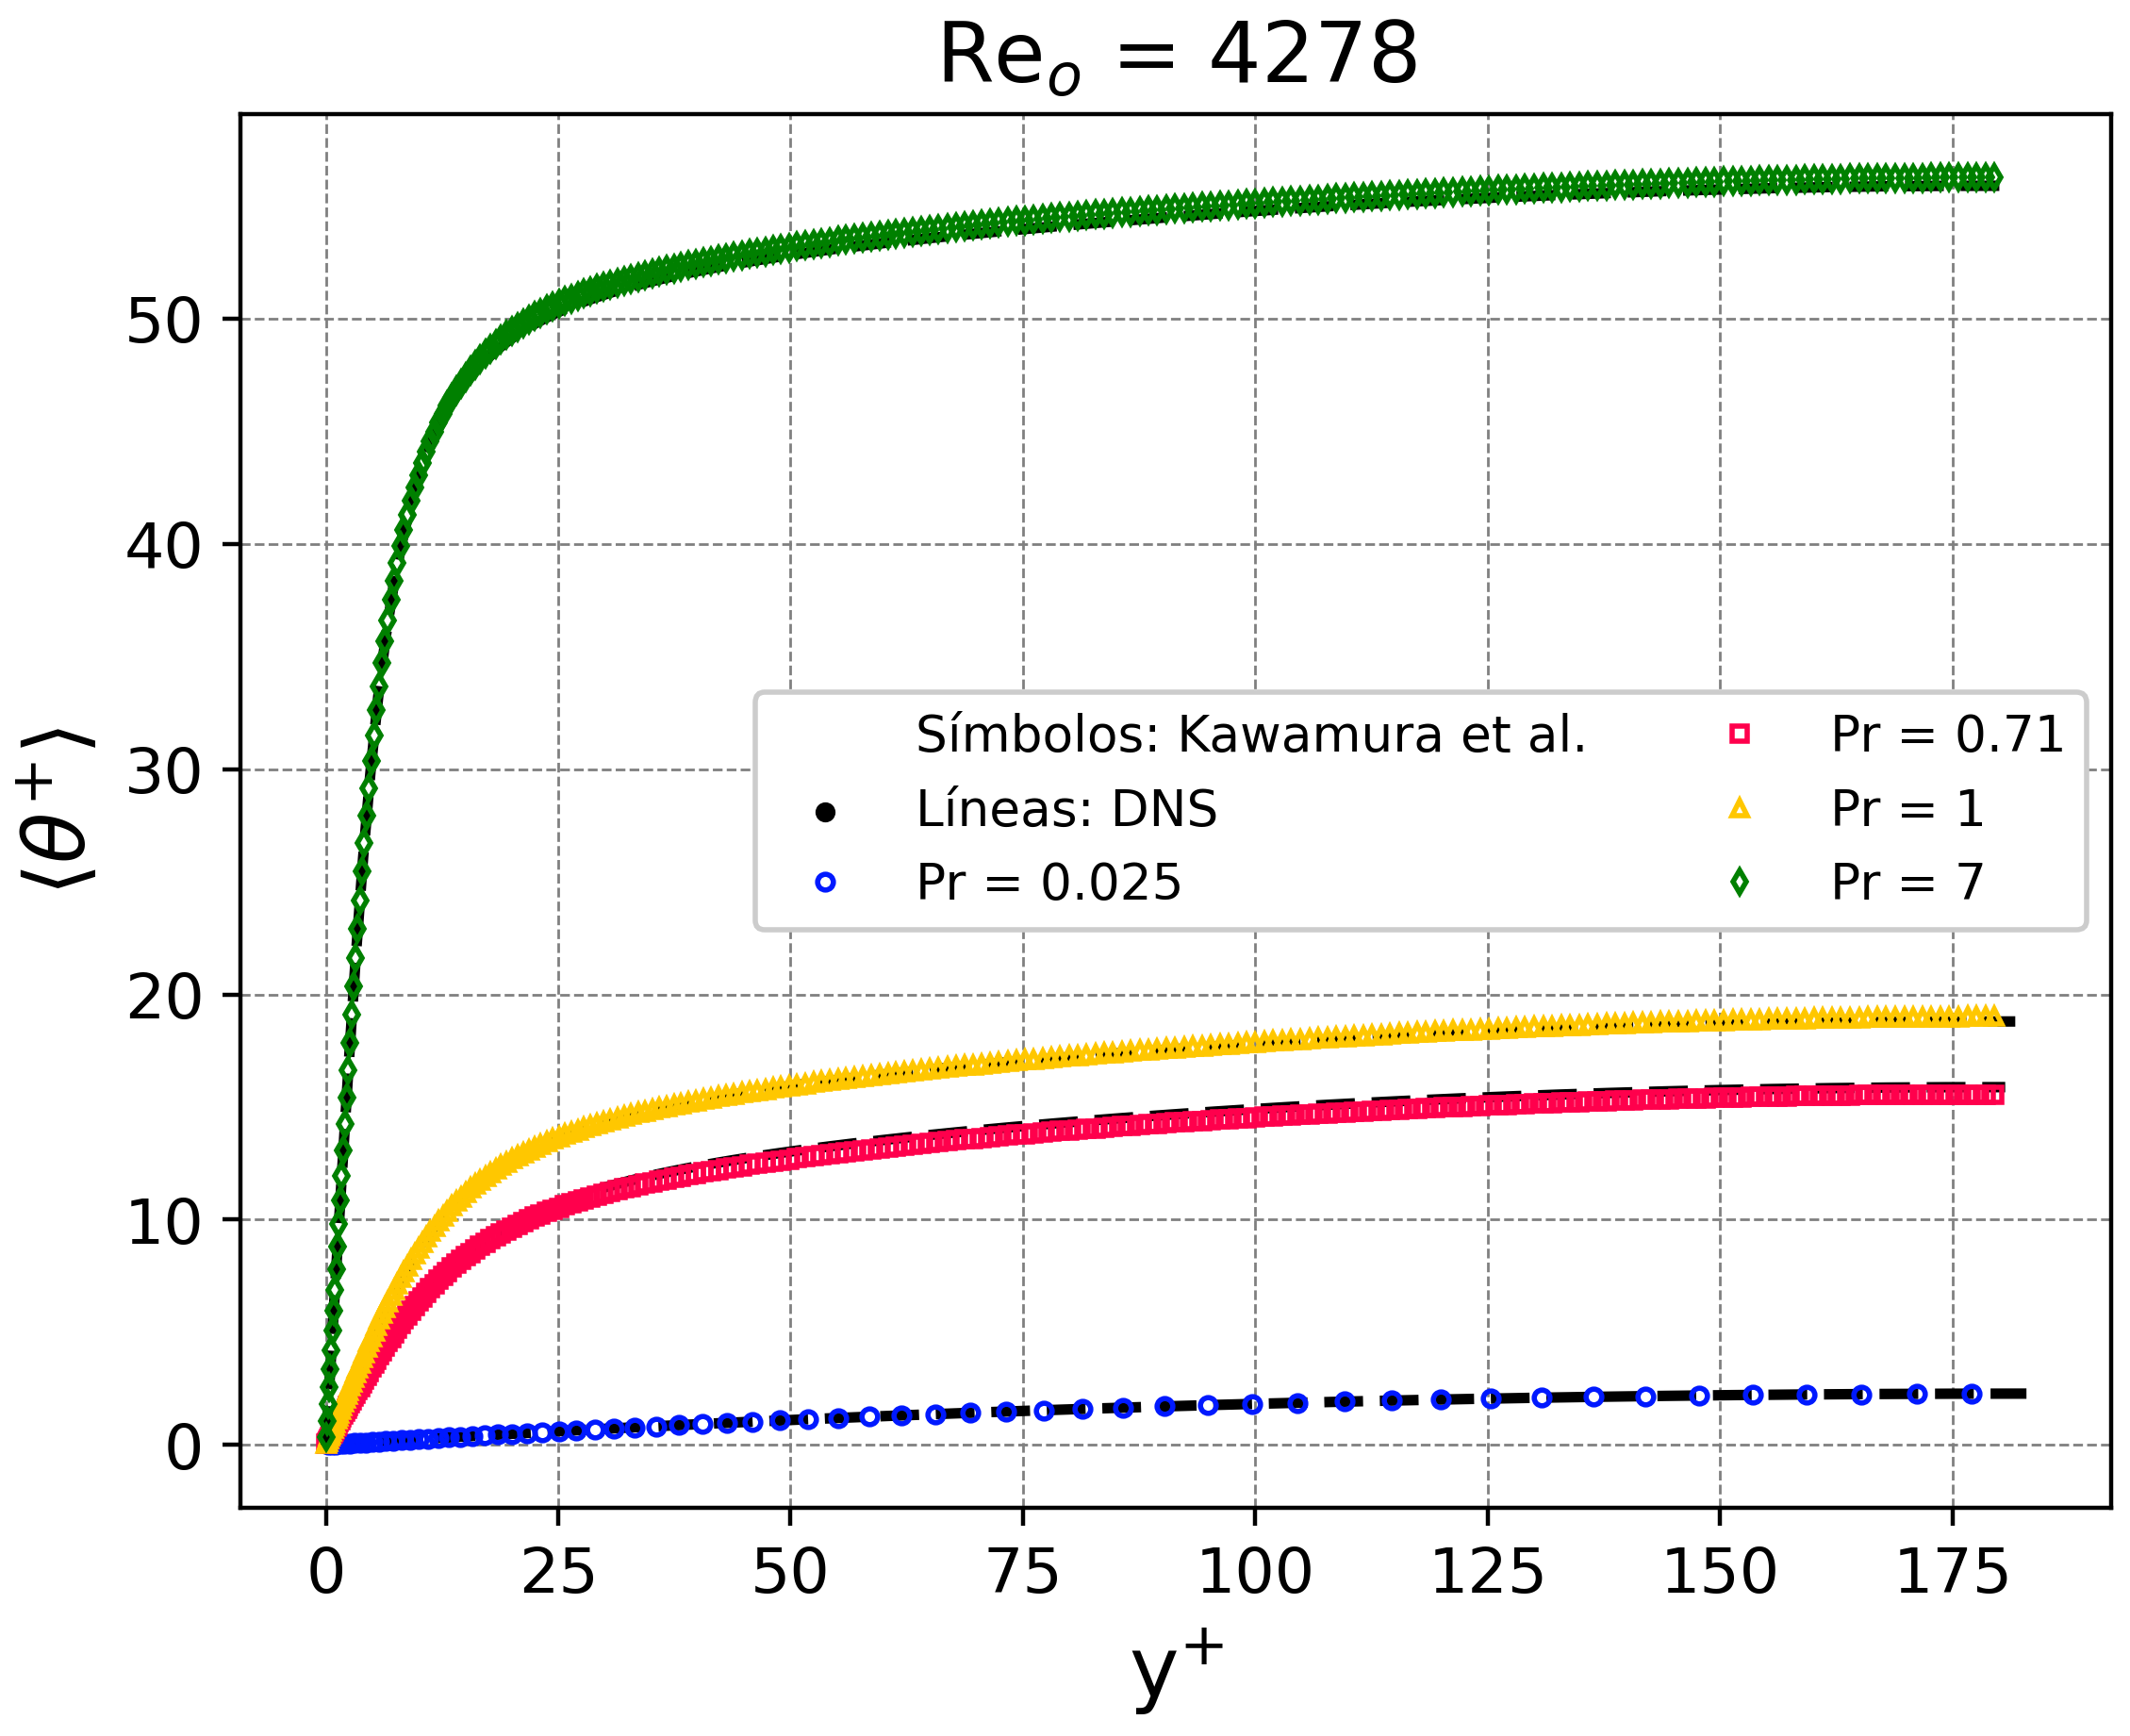
\includegraphics[width=0.49\textwidth]{figures/cap4/kawamura_prs/tep_theta.png}
    \label{fig:kpr-theta}}  
    \subfloat[]{
    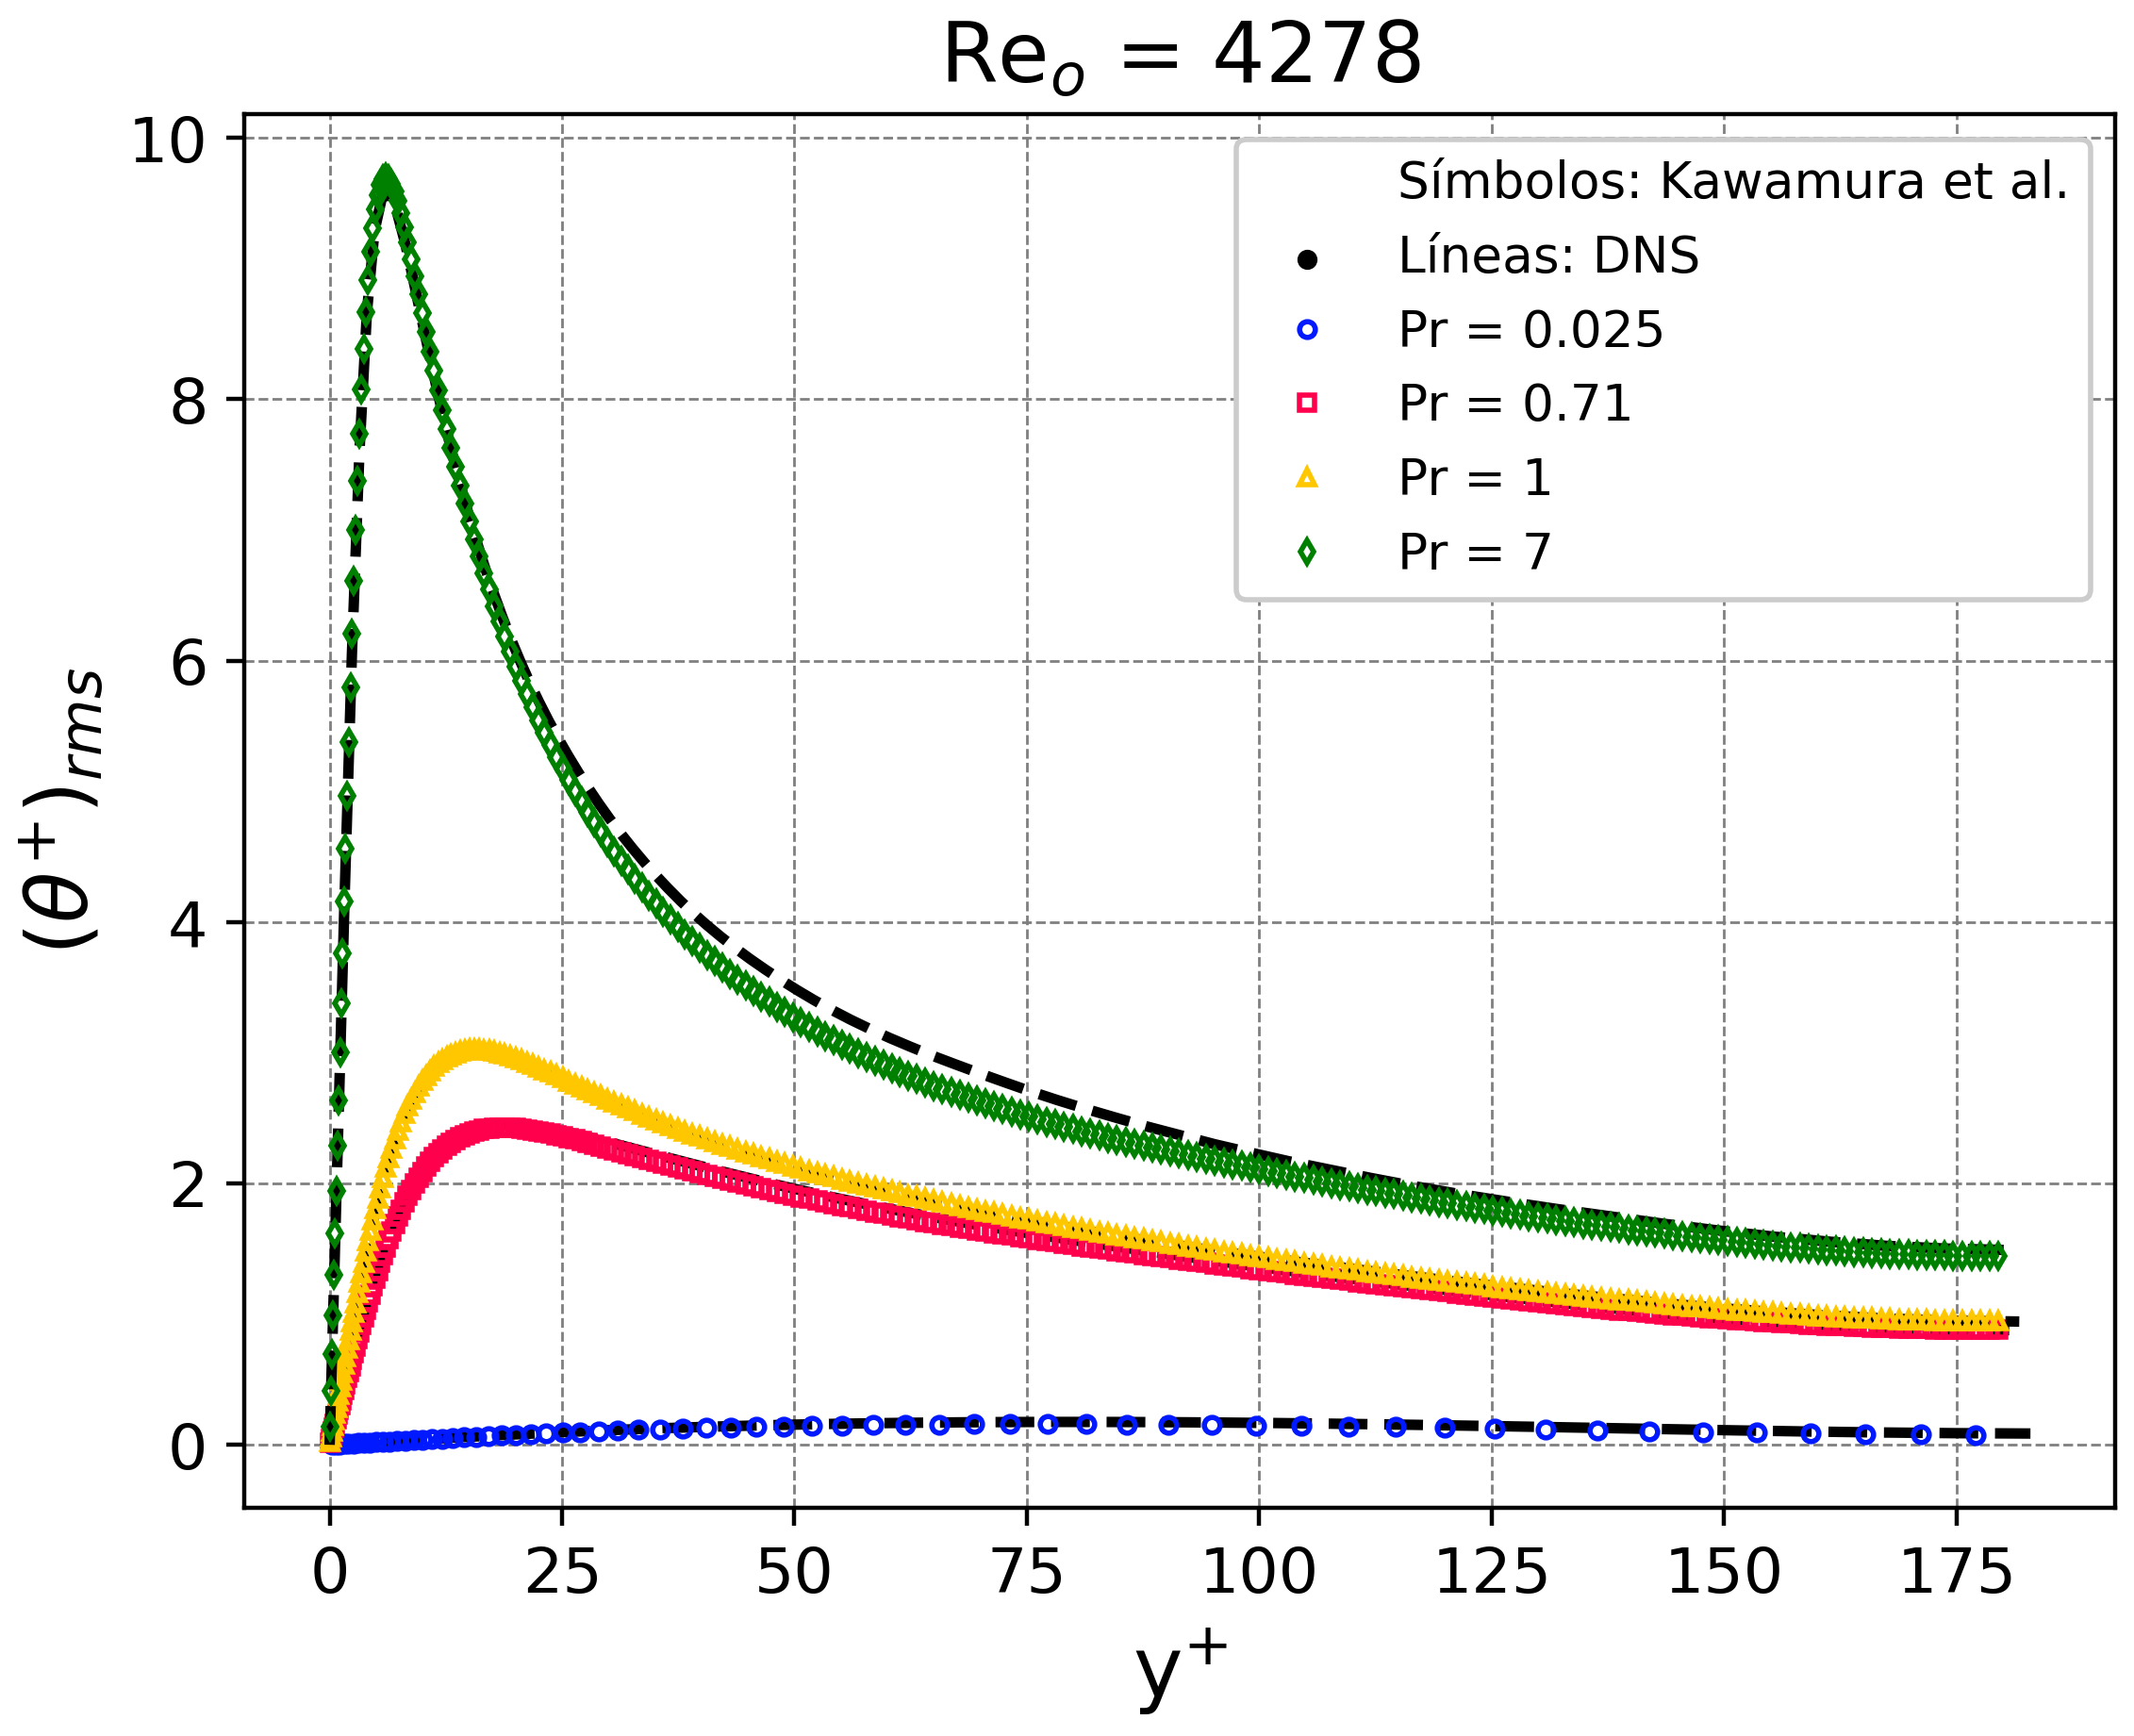
\includegraphics[width=0.49\textwidth]{figures/cap4/kawamura_prs/tep_thetap_rms.png}
    \label{fig:kpr-theta-rms}}  
 
  \subfloat[]{
    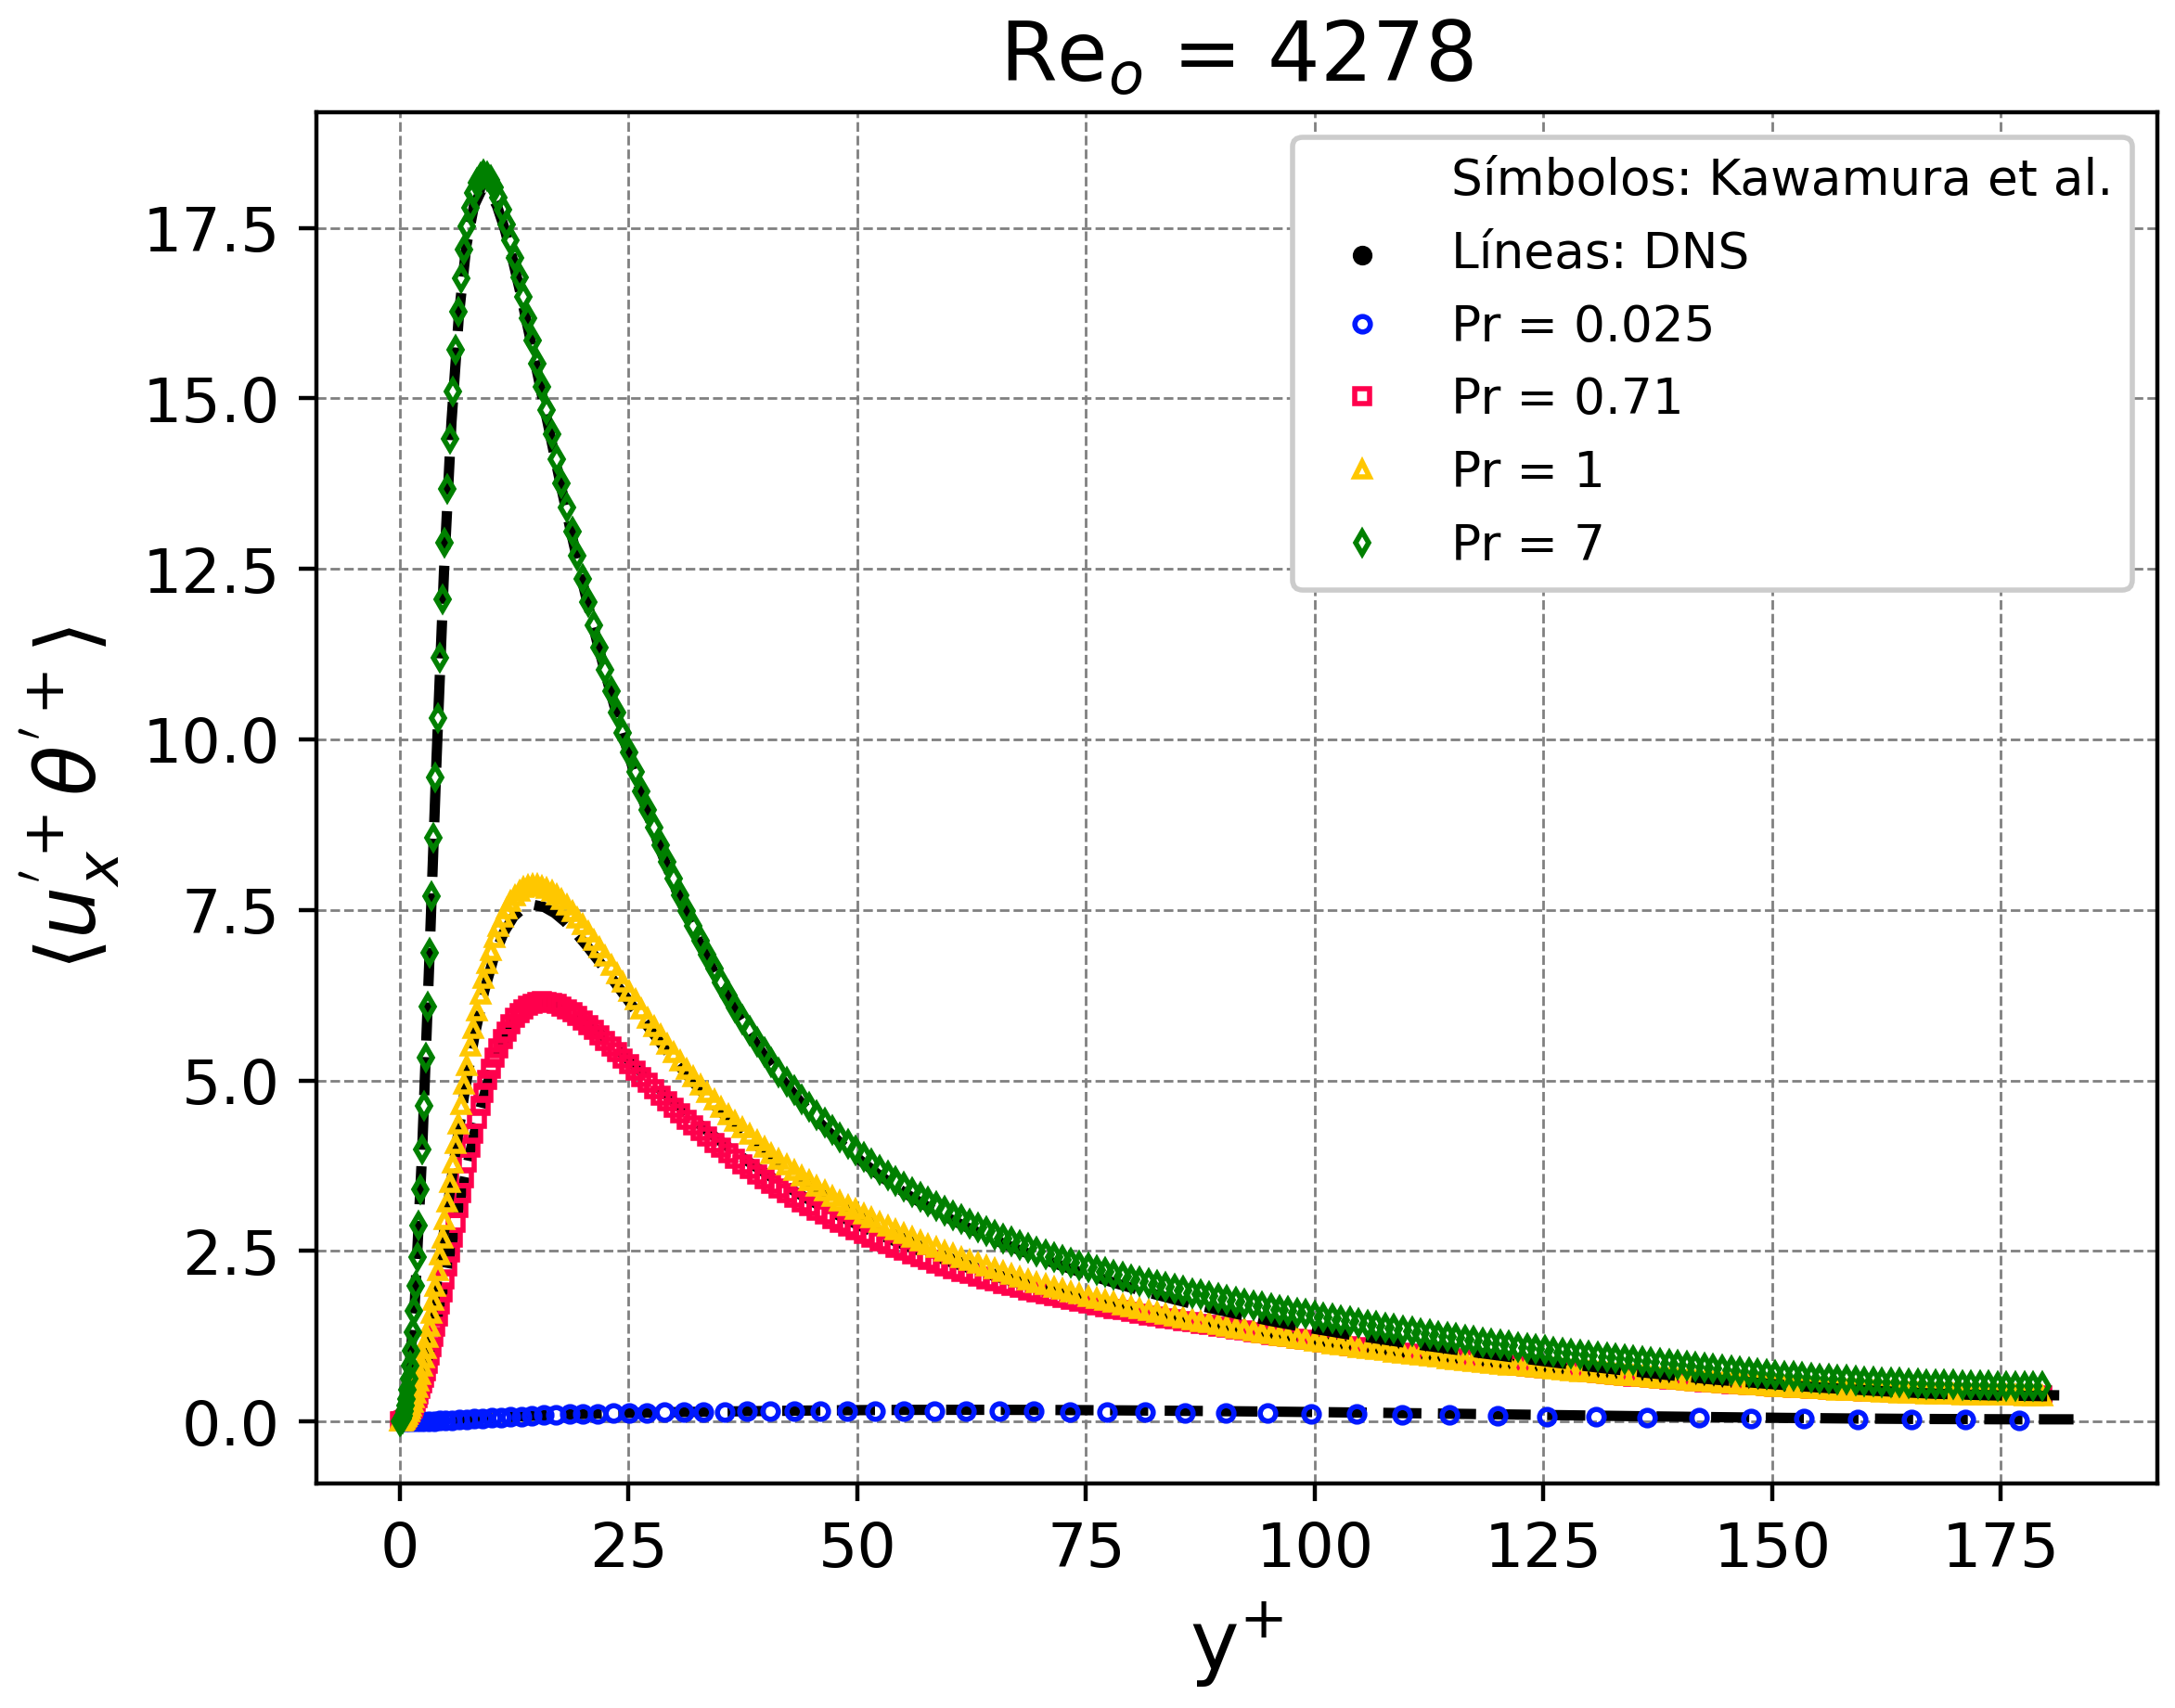
\includegraphics[width=0.49\textwidth]{figures/cap4/kawamura_prs/tep_up_thetap.png}
    \label{fig:kpr-ux-theta}}  
    \subfloat[]{
    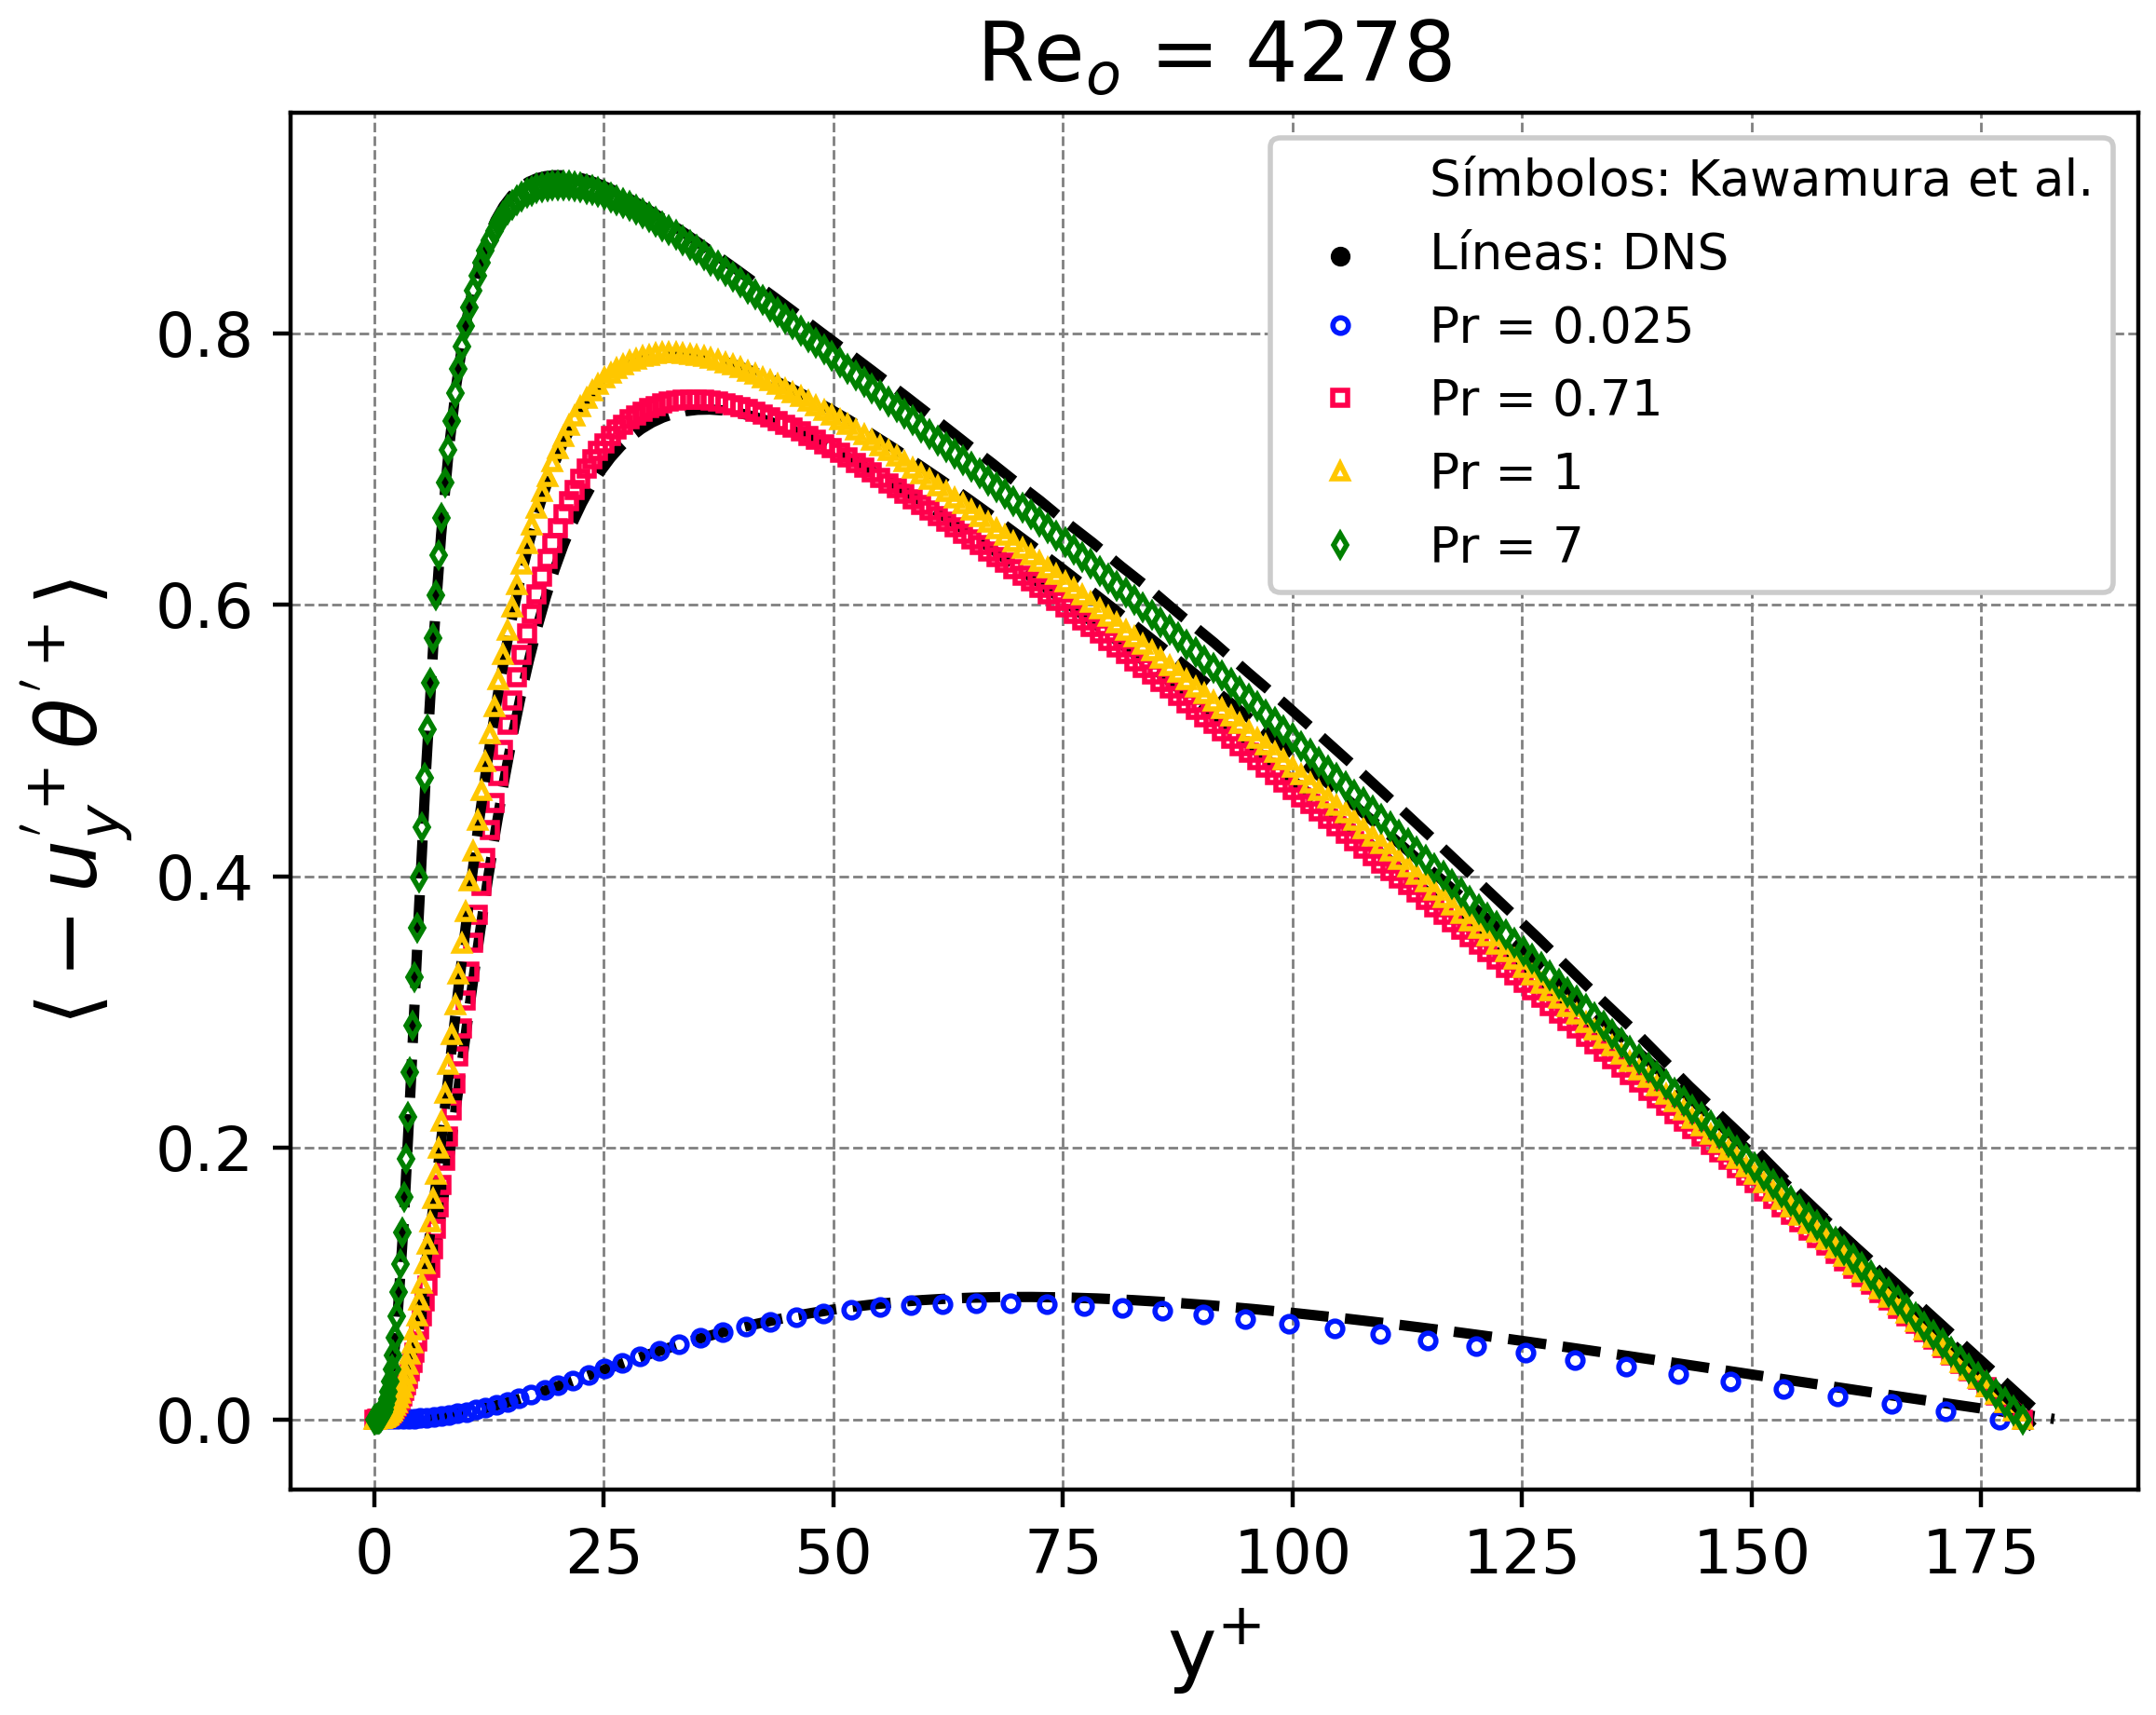
\includegraphics[width=0.49\textwidth]{figures/cap4/kawamura_prs/tep_vp_thetap.png}
    \label{fig:kpr-uy-theta}}  
 \caption{Para diferentes números de Pr se tienen los perfiles de \textbf{(a)} temperatura adimensional media, \textbf{(b)} fluctuaciones RMS de la temperatura adimensional, \textbf{(c)} flujo de calor turbulento en la dirección X, $\langle u^+_x \theta^+ \rangle$, y \textbf{(d)} flujo de calor turbulento en la dirección Y, $\langle u^+_y \theta^+ \rangle$.} 
 \label{fig:kpr_1}
\end{figure}


\subsection{Situación III. Canal turbulento en régimen laminar con convección mixta y $q''_w$ constante} \label{sec:mix-laminar}

Hasta aquí, la herramienta numérica XC3D se ha validado en aspectos hidrodinámicos y térmicos bajo convección forzada. Como punto de partida hacia el régimen de convección mixta, se realizan simulaciones considerando un régimen laminar con Re$_o$=100, Pr=1 y distintos números de Rayleigh (Ra = -25, -100, 75, 150, 250) a fin de evaluar el desempeño de XC3D frente a la influencia de la fuerza boyante. En todas las simulaciones se utiliza la malla M0. A diferencia de los apartados anteriores, en estas simulaciones no se impone ninguna condición adicional en el flujo con la intención de acelerar el paso al régimen turbulento, ya que estamos tratando con soluciones laminares.

Se comparan los perfiles de velocidad \textit{streamwise} y de temperatura adimensional con las soluciones analíticas de Chen y Chung \cite{chen1996linear}, dadas por las ecuaciones \ref{eq:vel_asist_boyant} - \ref{eq:theta_opo_boyant}. Los mismos se encuentran en la forma adimensional descrita en el Capítulo \ref{cap:modelo}. En las Figuras \ref{fig:chen-ux} y \ref{fig:chen-theta}, las soluciones analíticas se muestran con anillos negros; asimismo, se incluye el caso con $\text{Ra}=0$ ($\Pi=0$) como referencia (línea azul a trazos). Se aprecia una excelente concordancia entre las soluciones analíticas y las simulaciones DNS, tanto para flujo descendente ($\text{Ra}<0$) como para flujo ascendente ($\text{Ra}>0$). En consecuencia, la malla M0 (la opción computacionalmente más económica) reproduce con alta fidelidad las soluciones laminares de Chen y Chung. 

\begin{figure}[H]
 \centering
  \subfloat[]{
    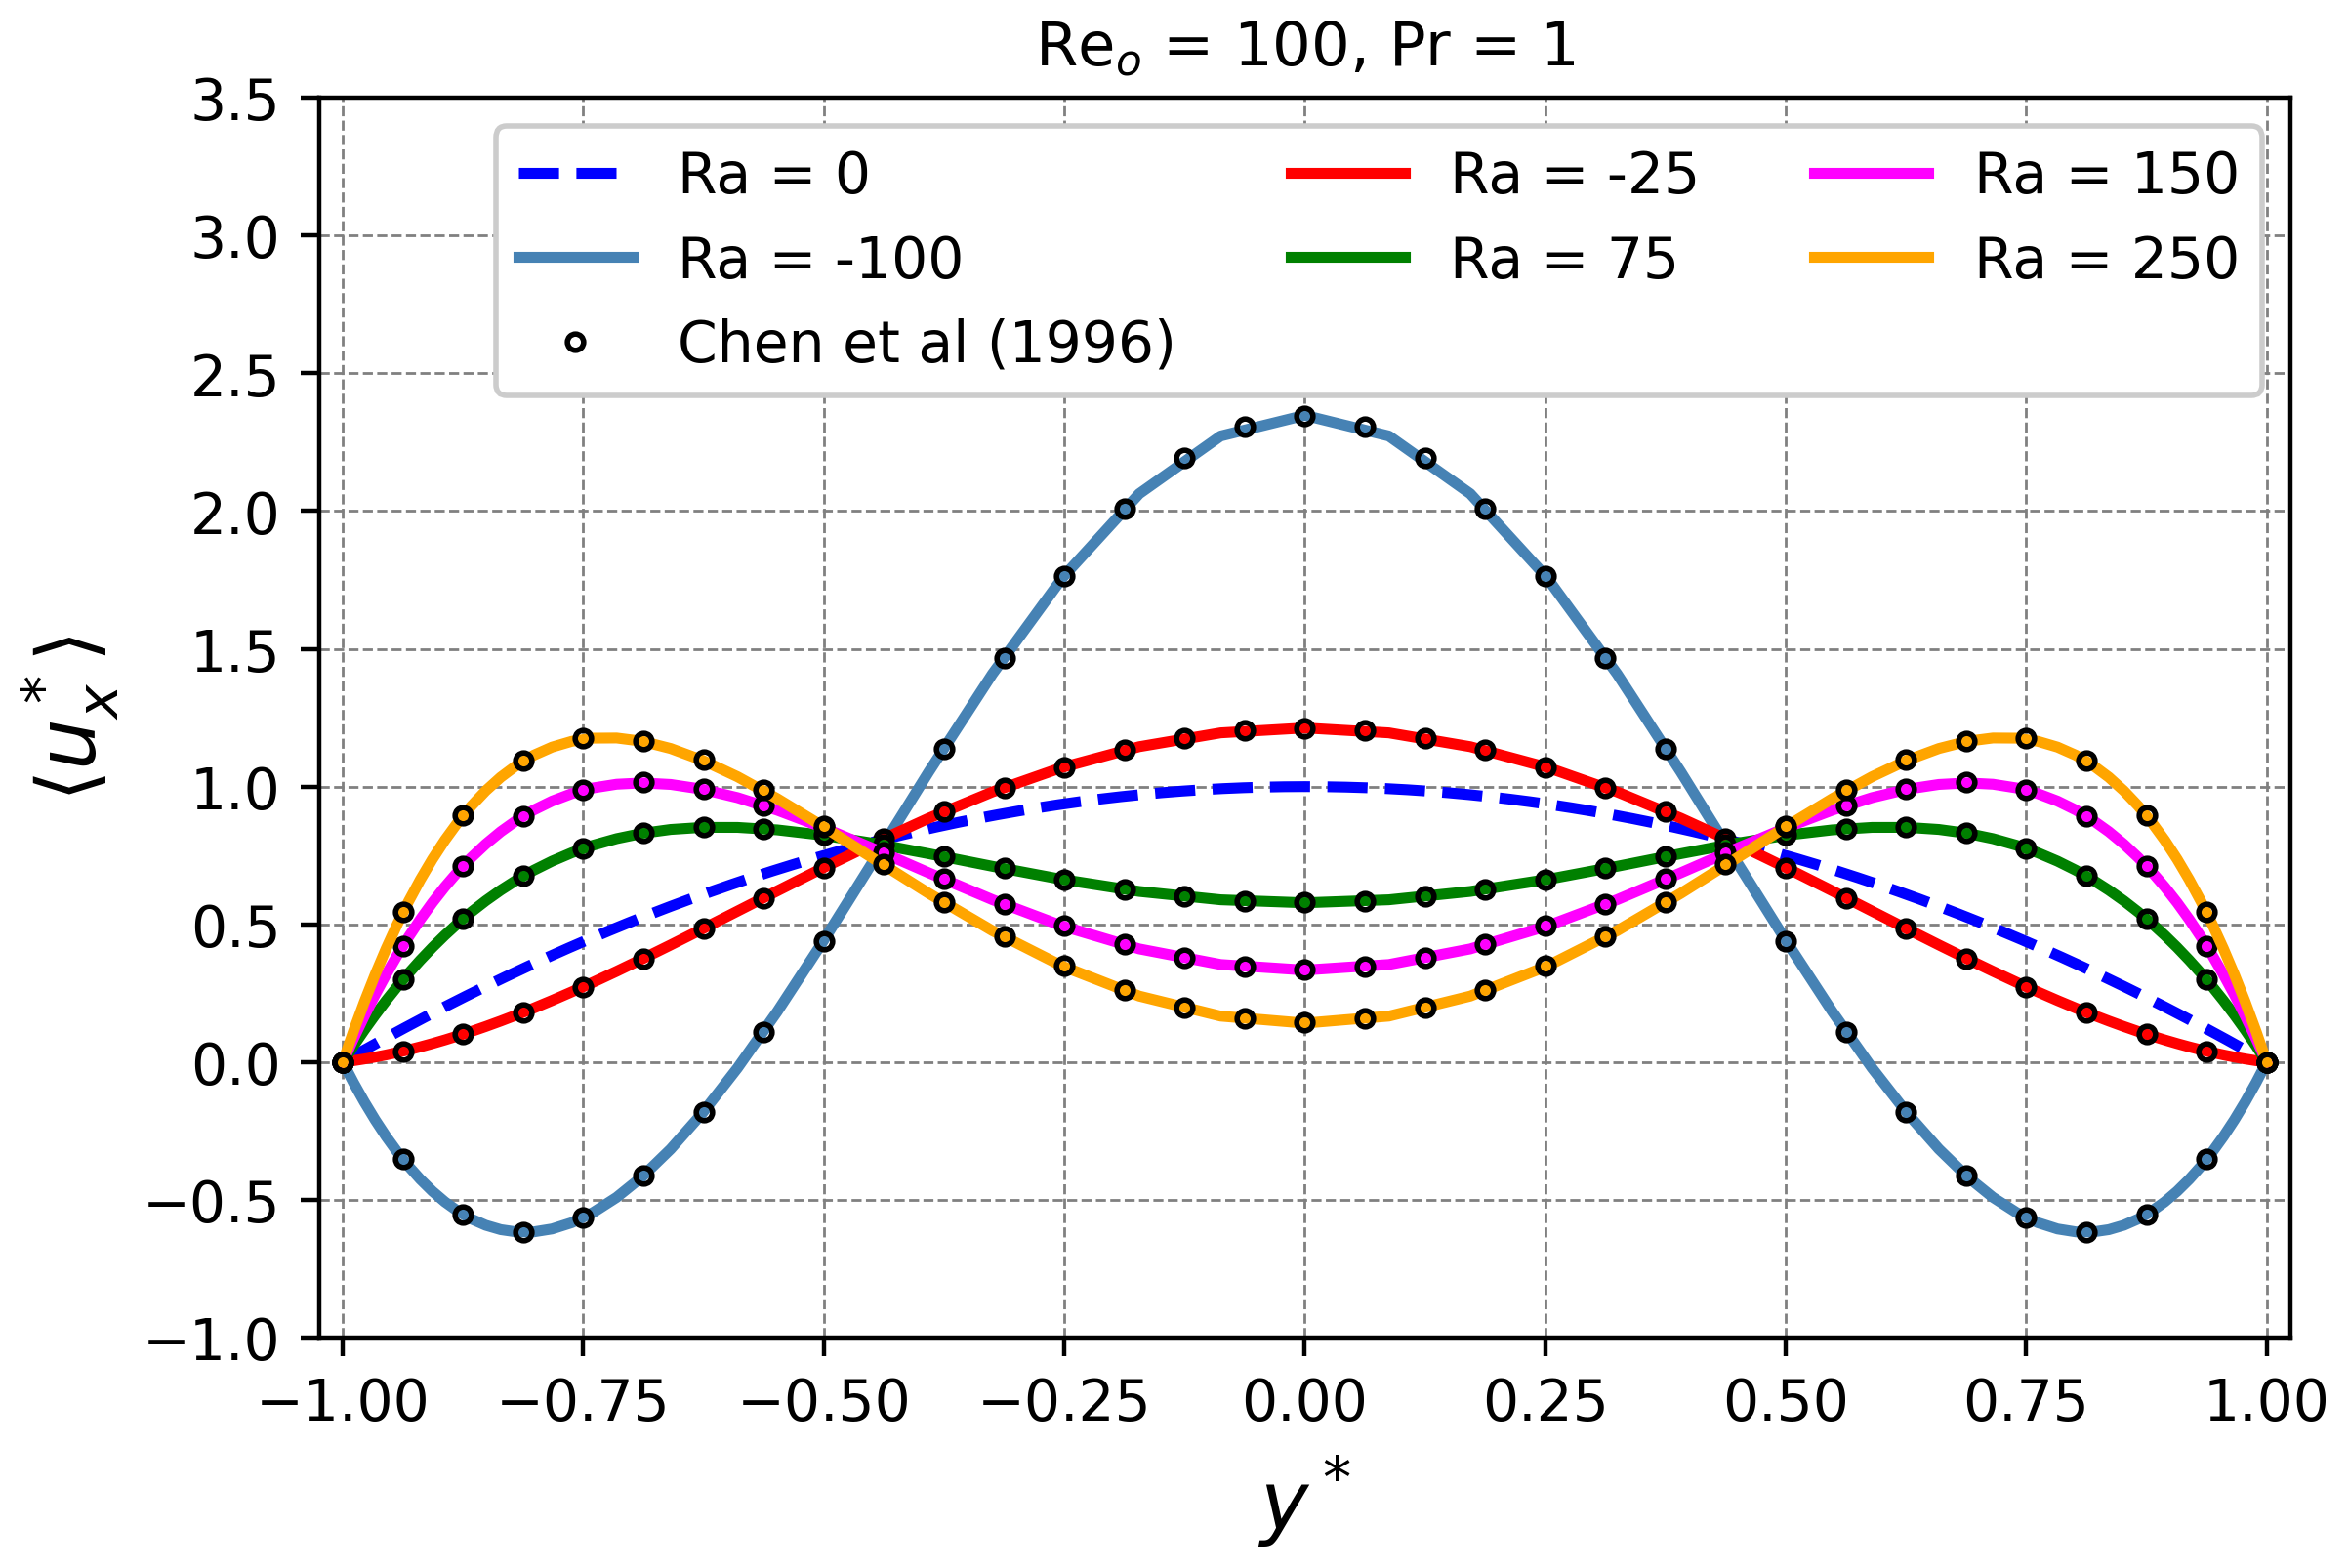
\includegraphics[width=0.5\textwidth]{figures/cap4/laminar/ux_mean.png}
    \label{fig:chen-ux}}  
    \subfloat[]{
    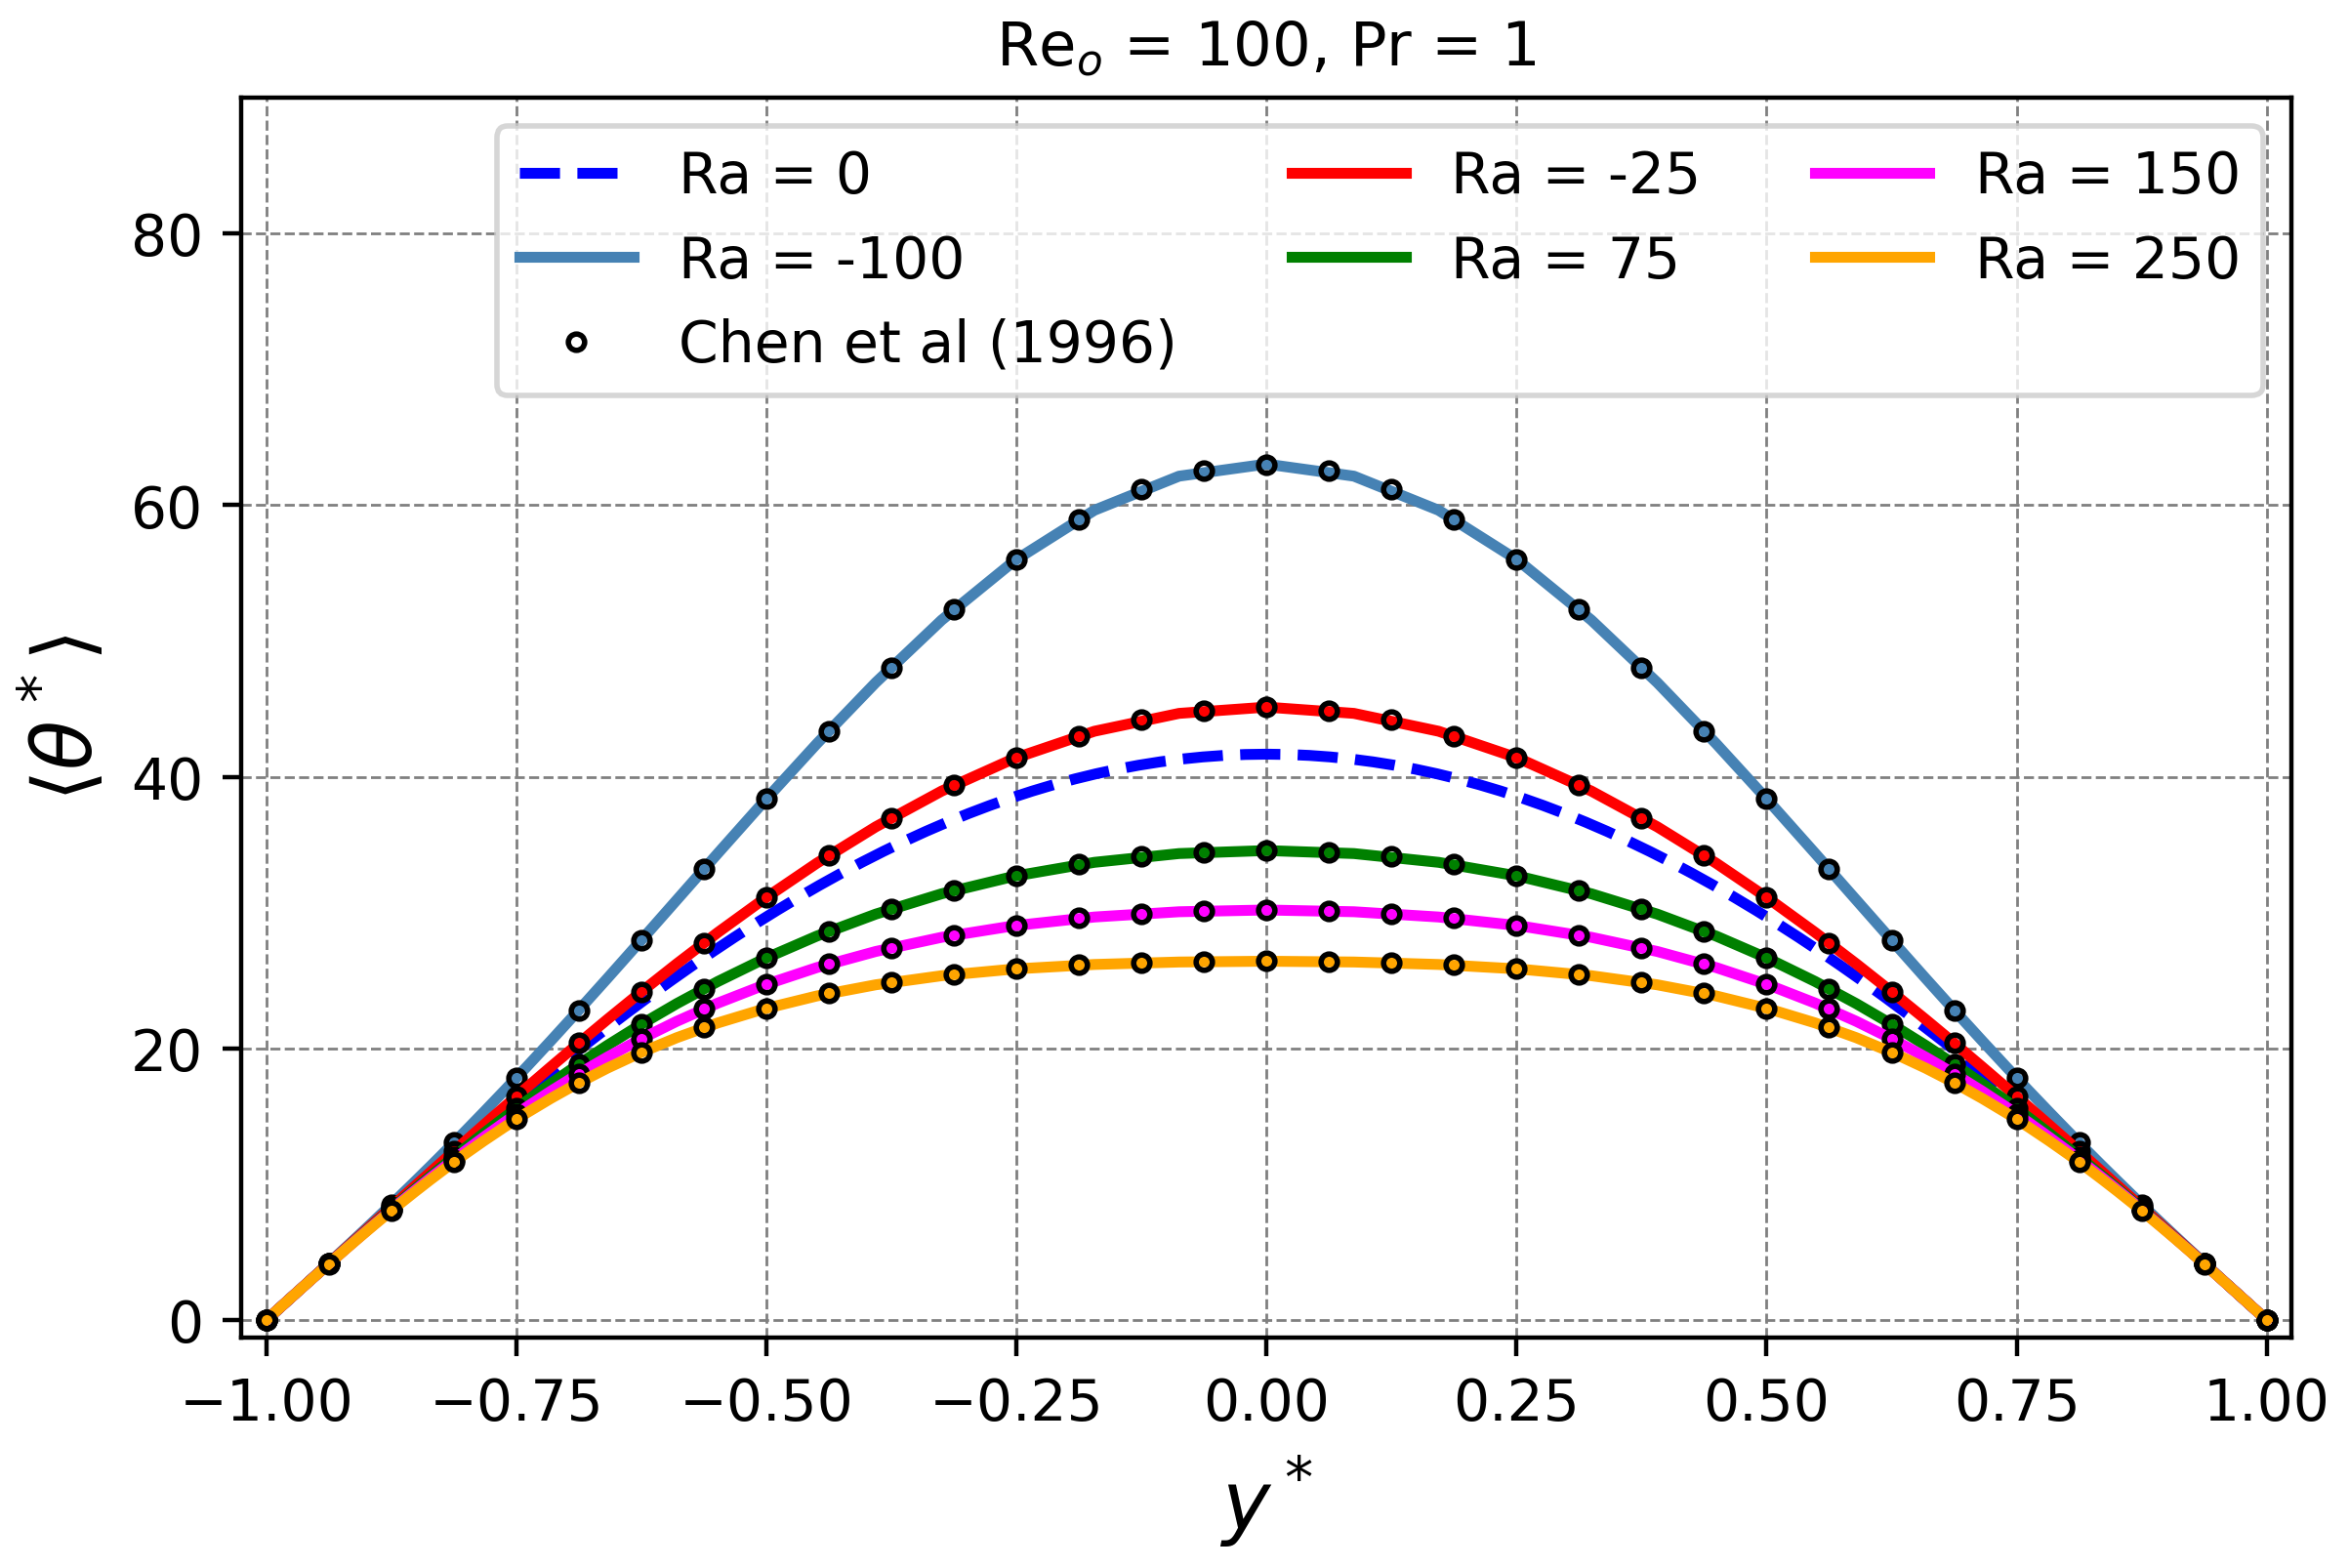
\includegraphics[width=0.5\textwidth]{figures/cap4/laminar/theta_mean.png}
    \label{fig:chen-theta}}  
 \caption{Perfiles de: \textbf{(a)} velocidad y \textbf{(b)} temperatura, considerando distintos casos en régimen laminar con convección mixta.} 
 \label{fig:chen-profiles}
\end{figure}


\subsection{Situación IV. Canal turbulento en convección mixta con $\Delta T$ constante entre paredes.}

\textit{\textbf{Observación inicial}: al momento de realizar las simulaciones para validar la implementación del término de fuerza boyante en XC3D, no se encontraban disponibles en la literatura datos de referencia. En particular, faltaban datos para canales rectangulares con flujo turbulento en régimen de convección mixta, ascendente o descendente, y con flujo de calor impuesto en las paredes. La alternativa disponible utilizada fue el trabajo de Guo \textit{et al.} \cite{guo2022direct} basado en un sistema físico conceptualmente diferente\footnote{En ese sentido, las ecuaciones de gobierno empleadas en el trabajo de Guo \textit{et al.} son ligeramente diferentes a nuestras ecuaciones de gobierno \ref{eq:gob_system_adim}. Por ejemplo, una diferencia que destaca es que, al considerar paredes isotérmicas a distinta temperatura, el término fuente en la ecuación de energía es nulo.} (paredes isotérmicas a distinta temperatura). Más recientemente, tomamos conocimiento del trabajo de Zhou \textit{et al.} \cite{zhou2024direct} que presenta datos DNS con las mismas condiciones de borde empleadas en este trabajo.}


\begin{figure}[H]
 \centering
  \subfloat[]{
    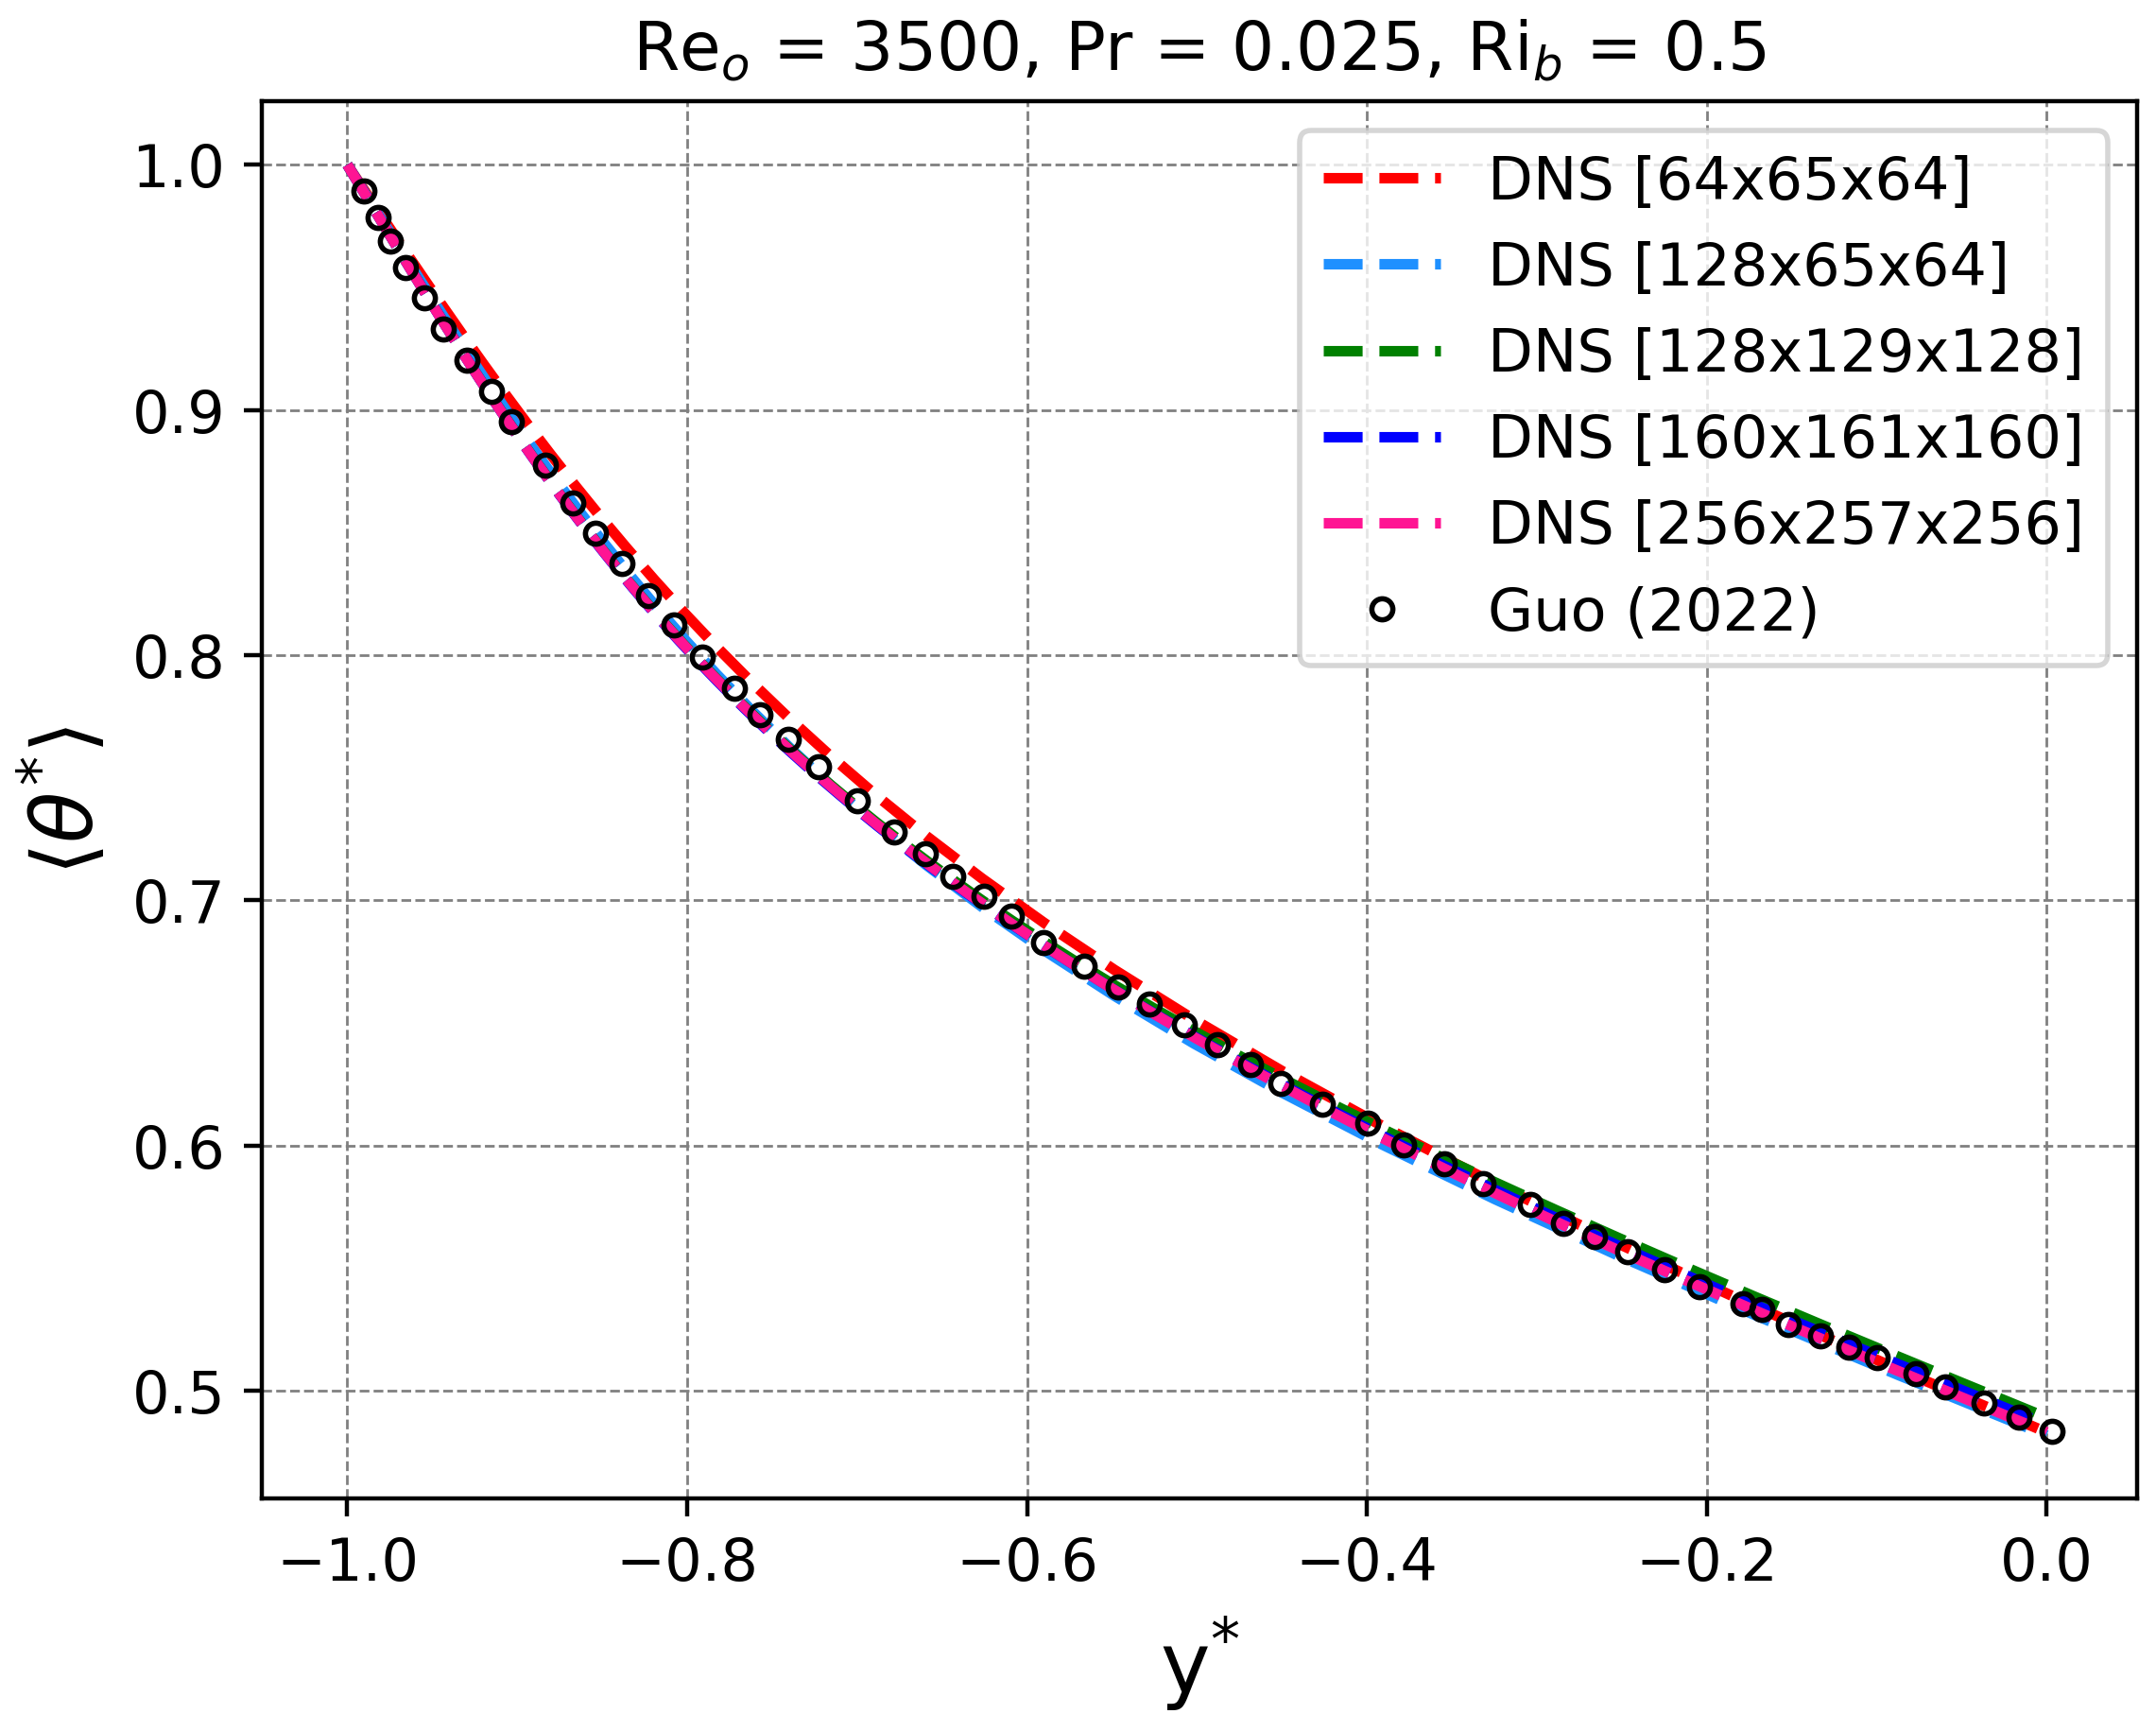
\includegraphics[width=0.49\textwidth]{figures/cap4/guo/Rib05/mct_theta.png}
   		\label{fig:guo-05-theta}}  
    \subfloat[]{
    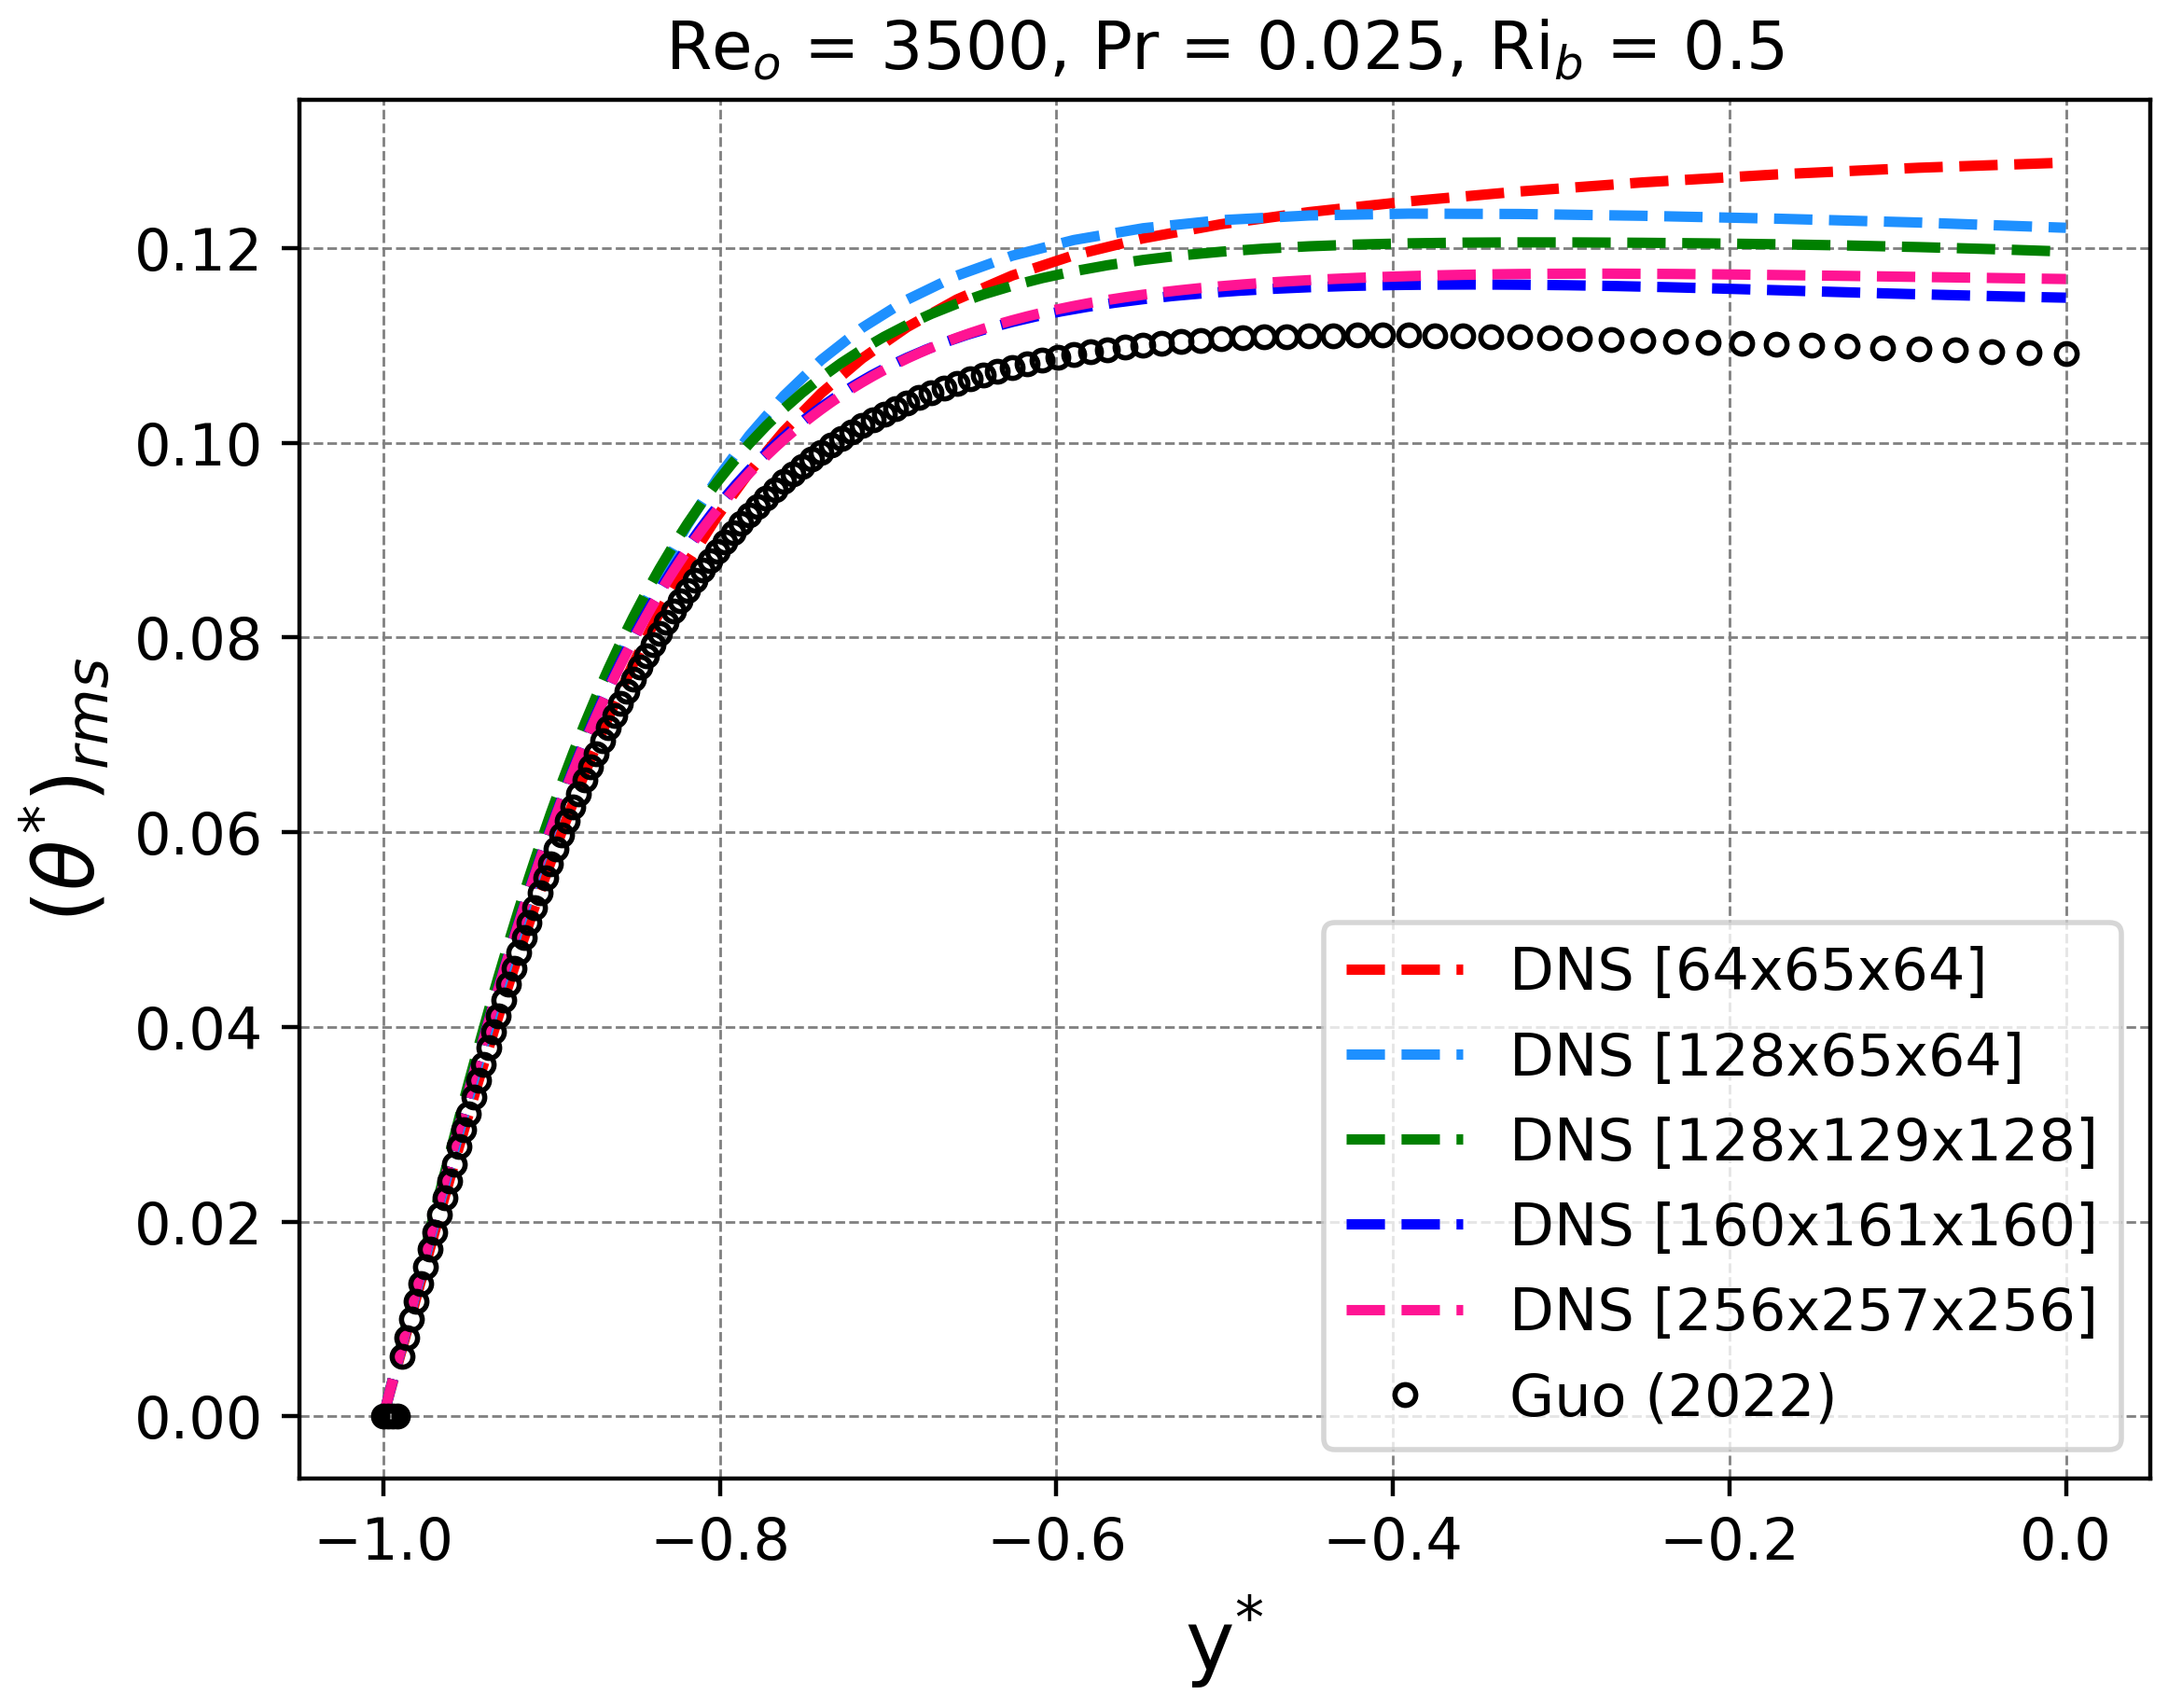
\includegraphics[width=0.49\textwidth]{figures/cap4/guo/Rib05/mct_thetap_rms.png}
  		\label{fig:guo-05-theta-rms}}  

  \subfloat[]{
    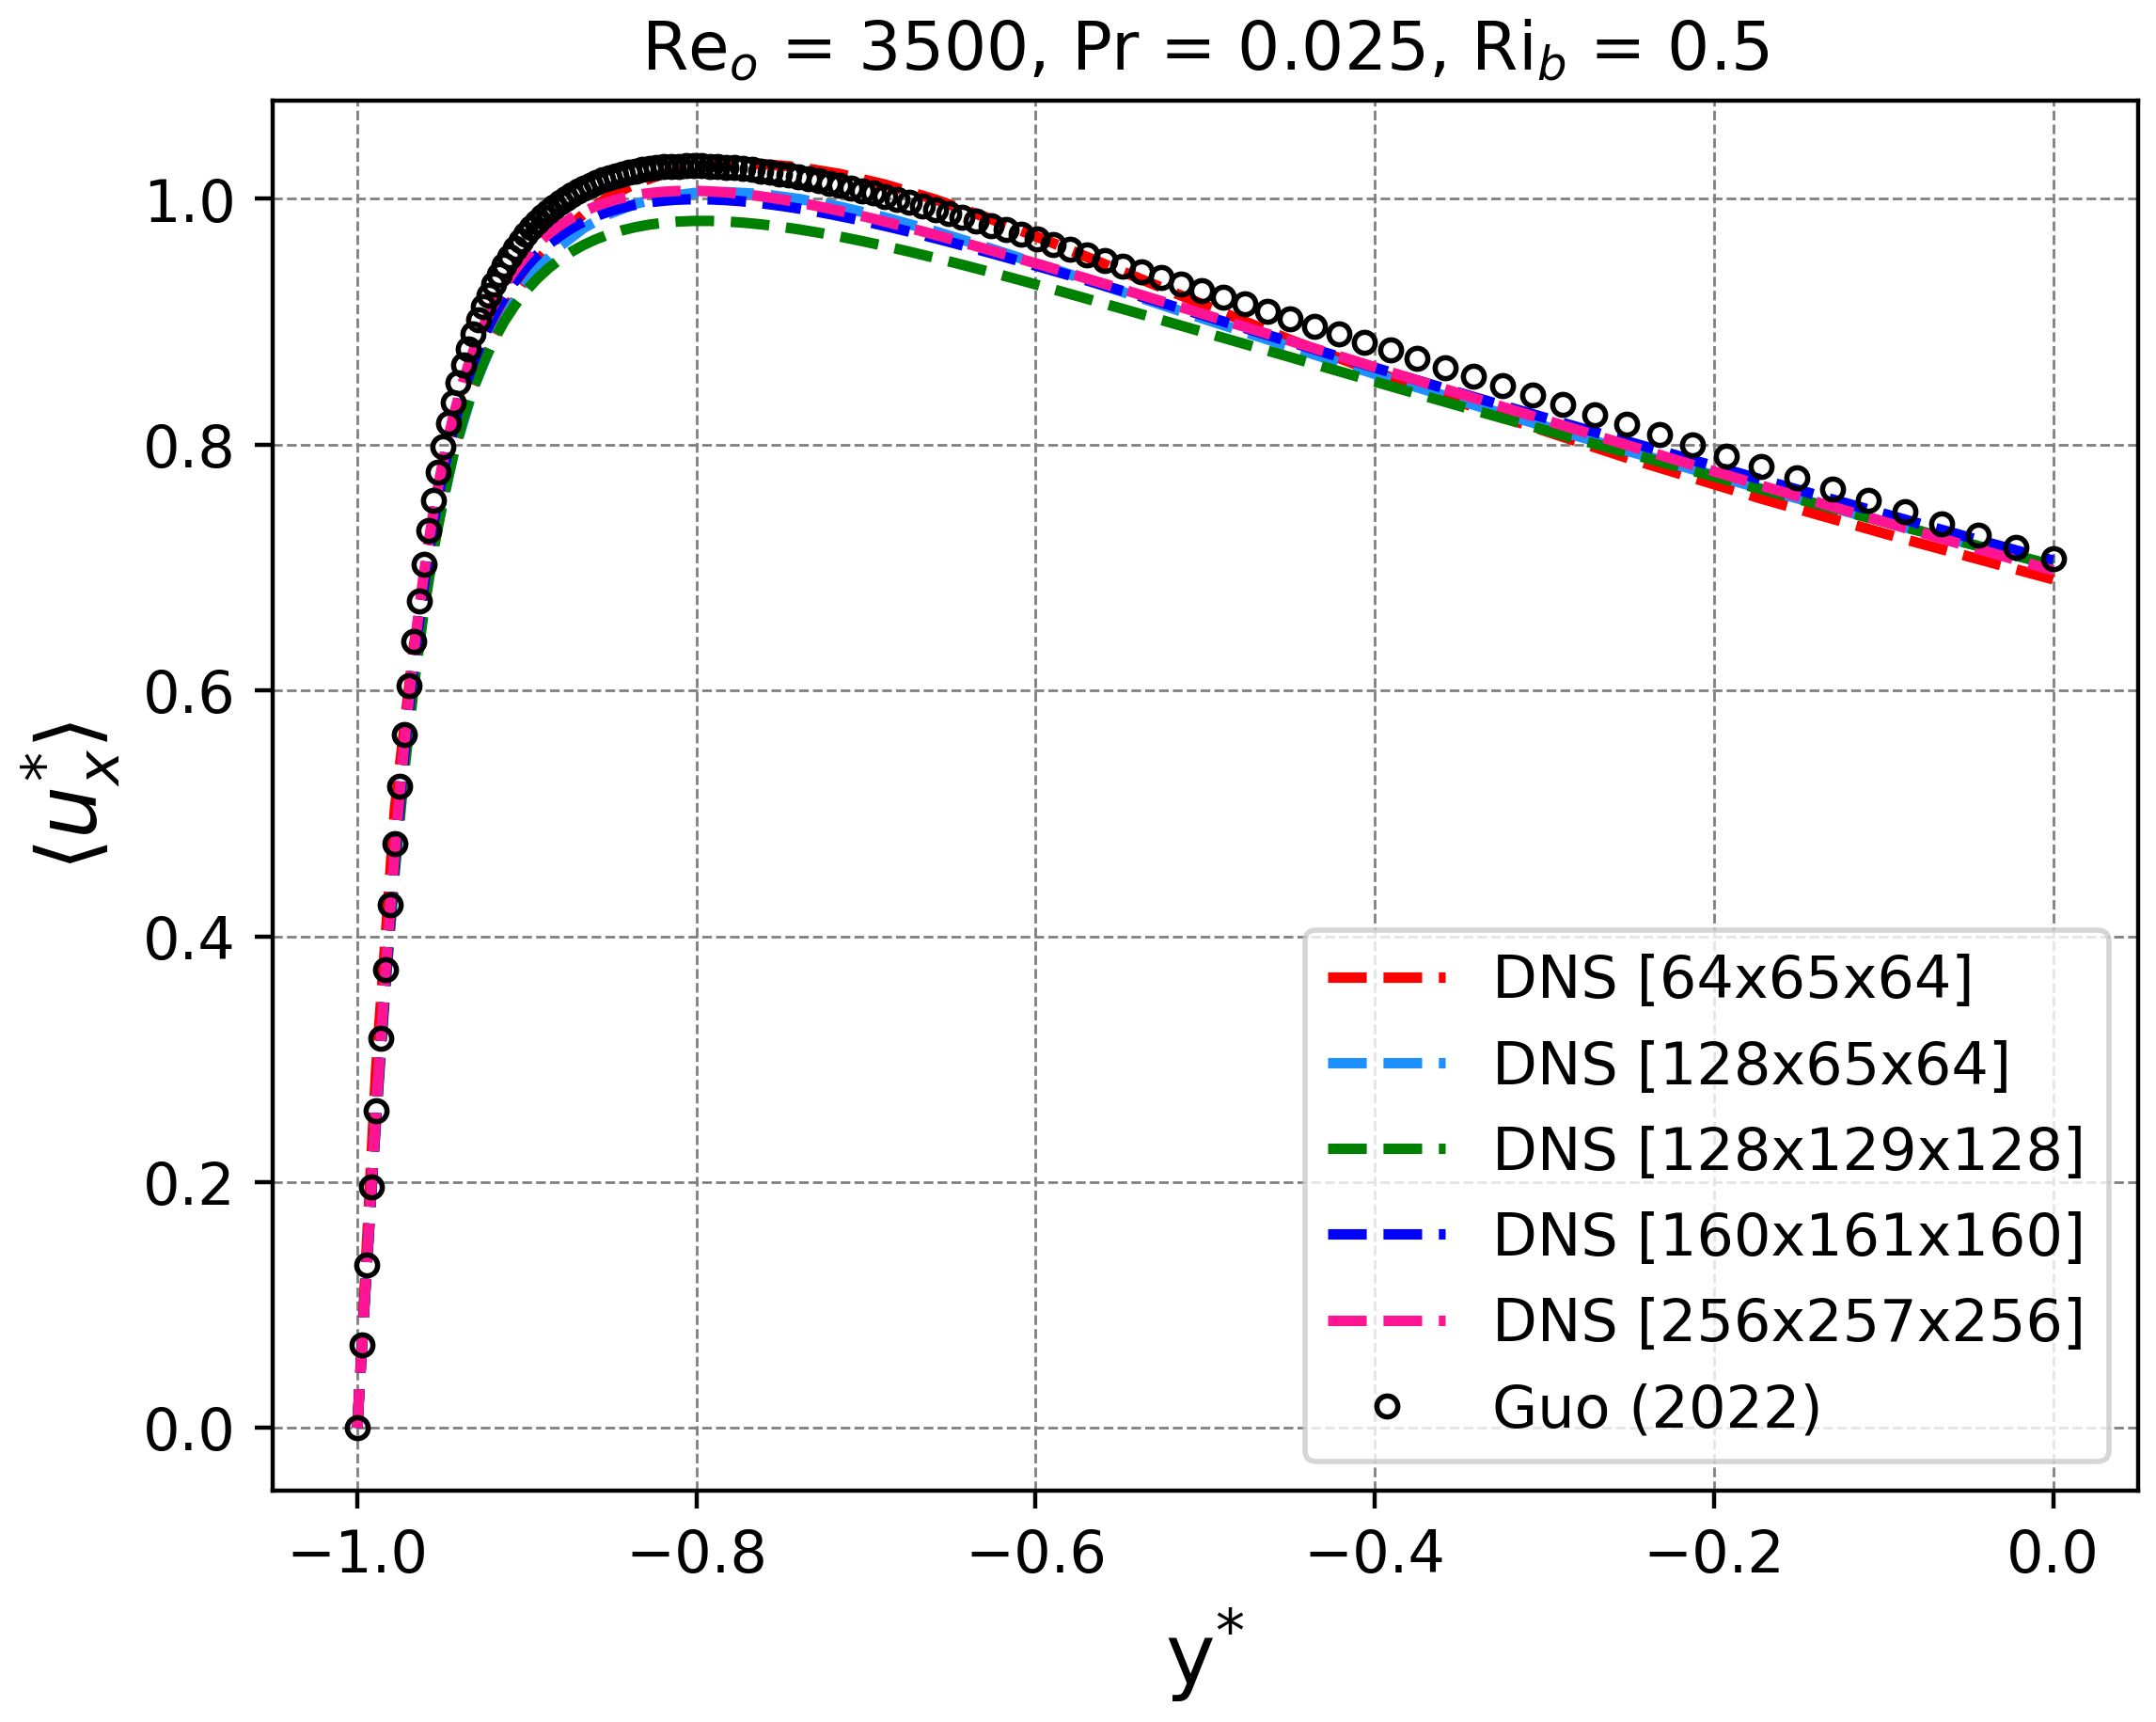
\includegraphics[width=0.49\textwidth]{figures/cap4/guo/Rib05/mct_upmean.png}
   		\label{fig:guo-05-ux}}  
    \subfloat[]{
    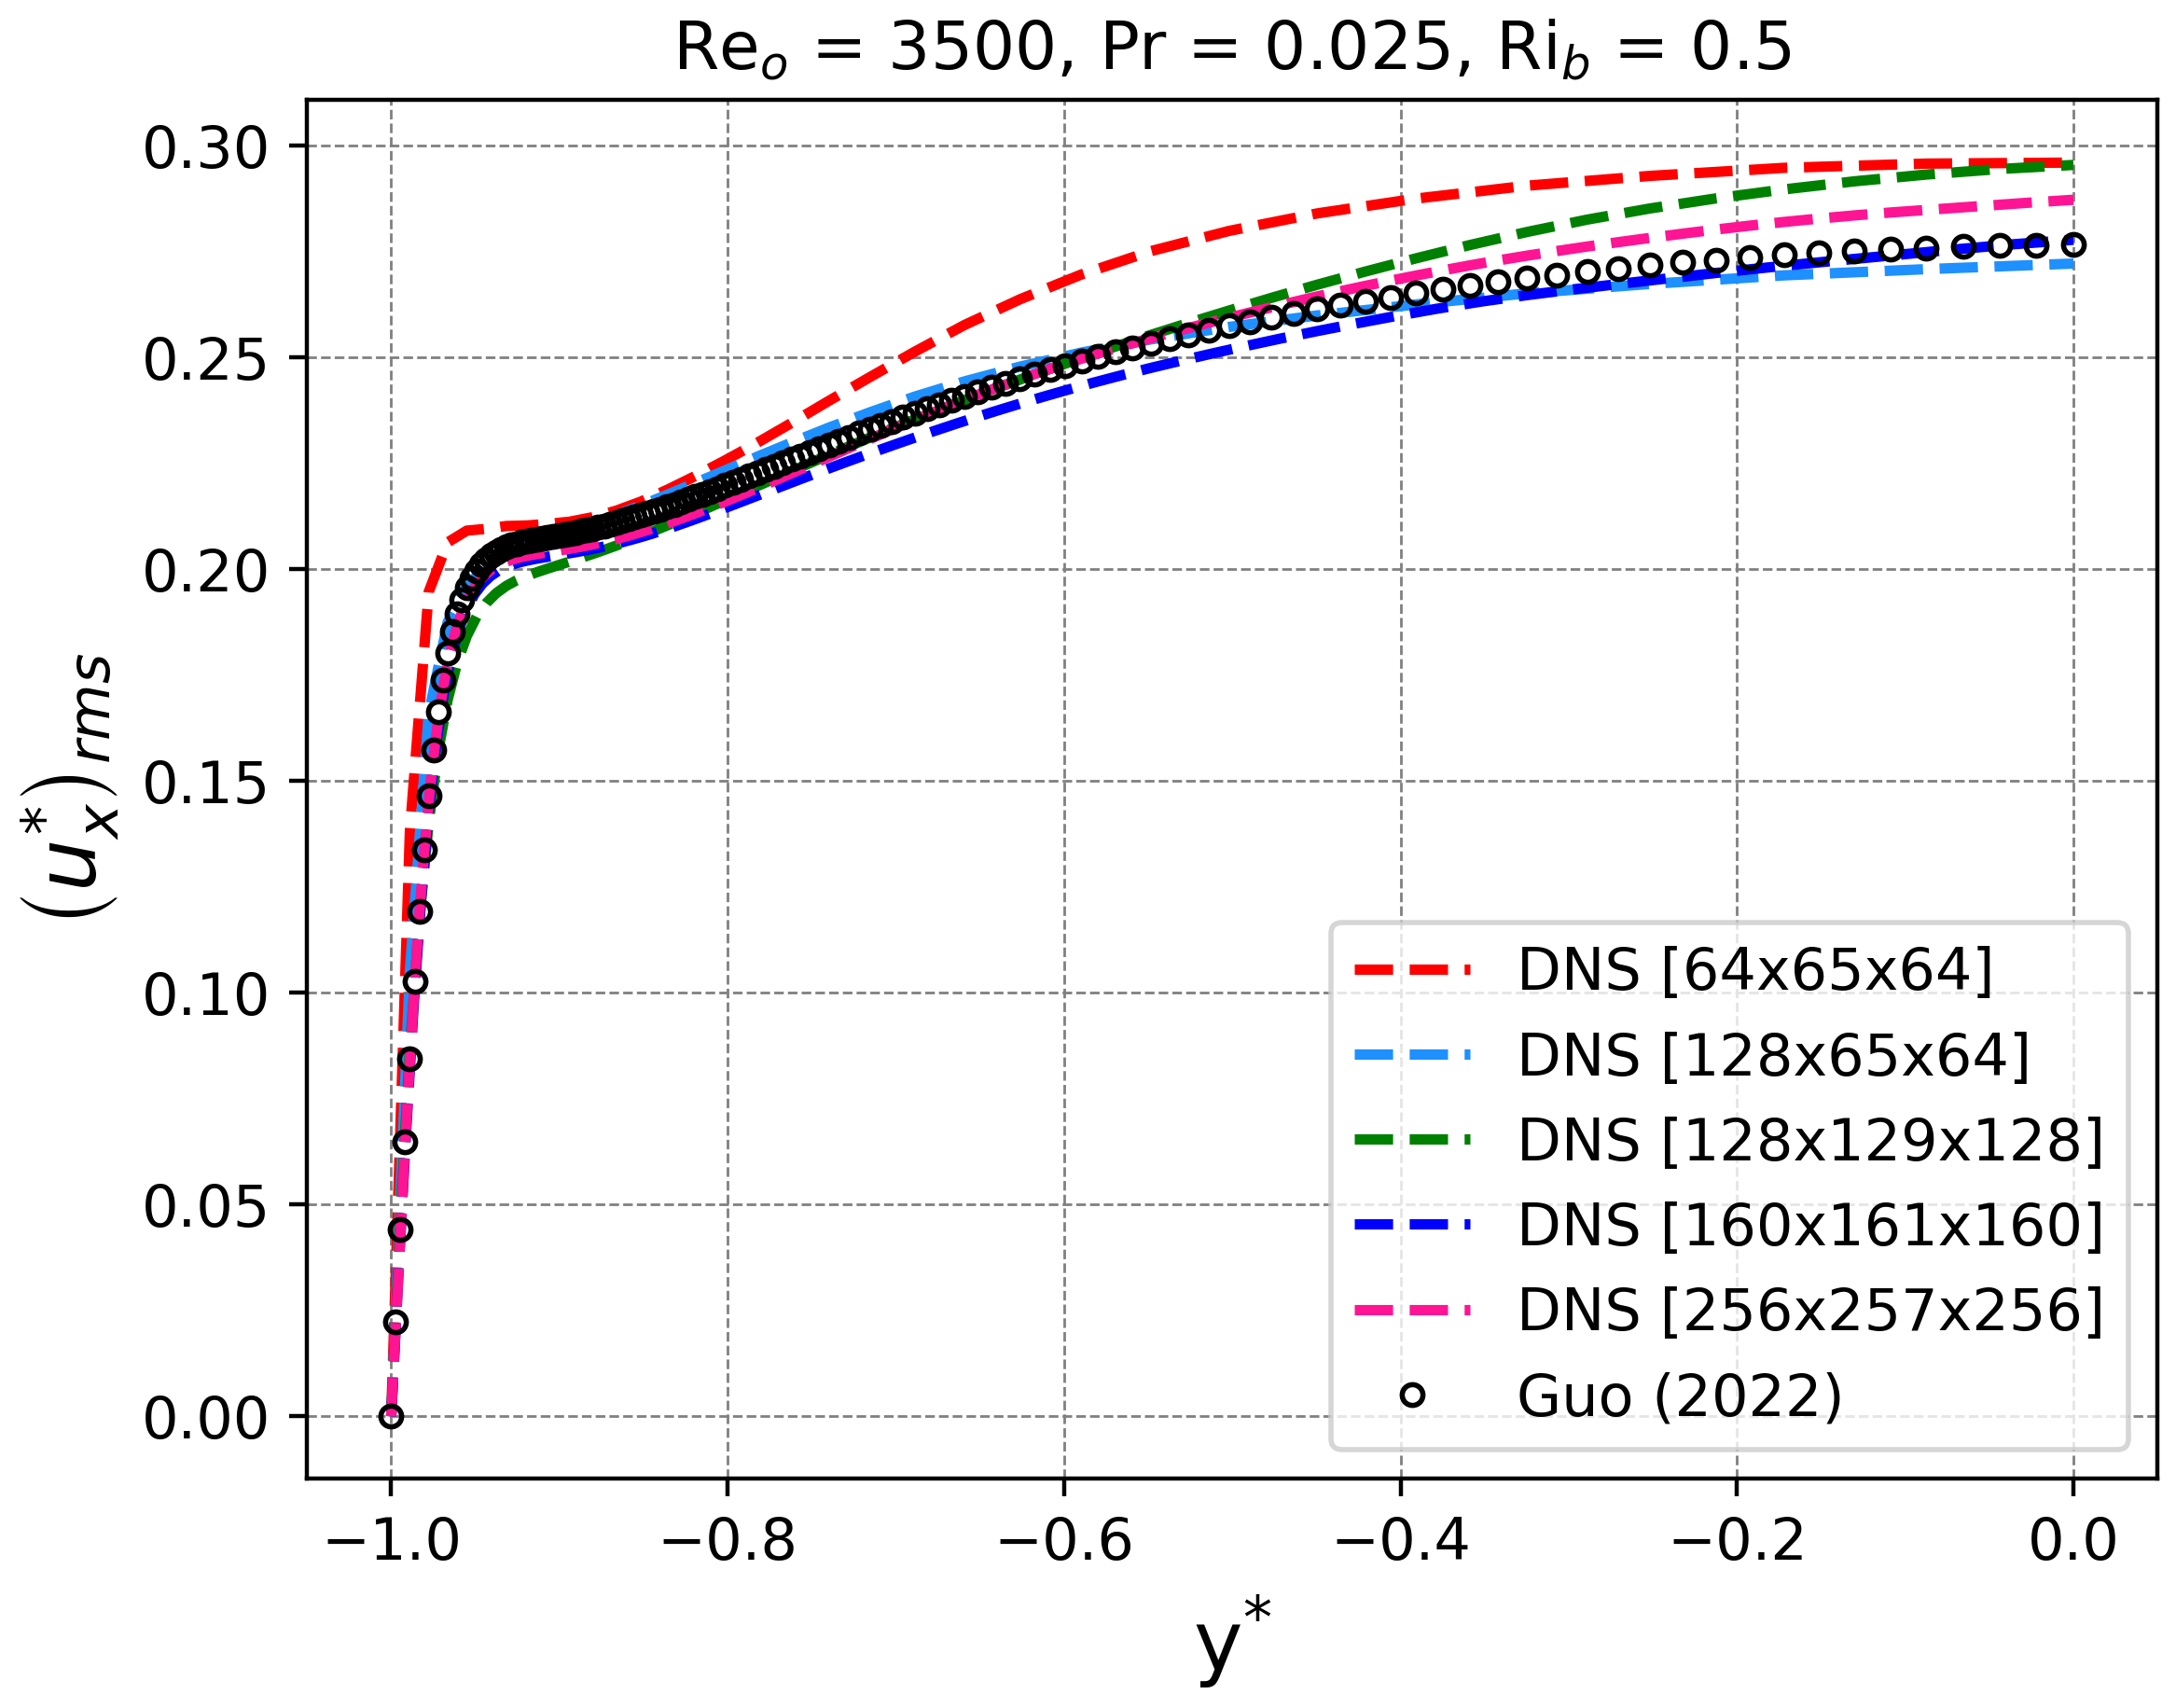
\includegraphics[width=0.49\textwidth]{figures/cap4/guo/Rib05/mct_uprms.png}
    	\label{fig:guo-05-ux-rms}}  

  \subfloat[]{
    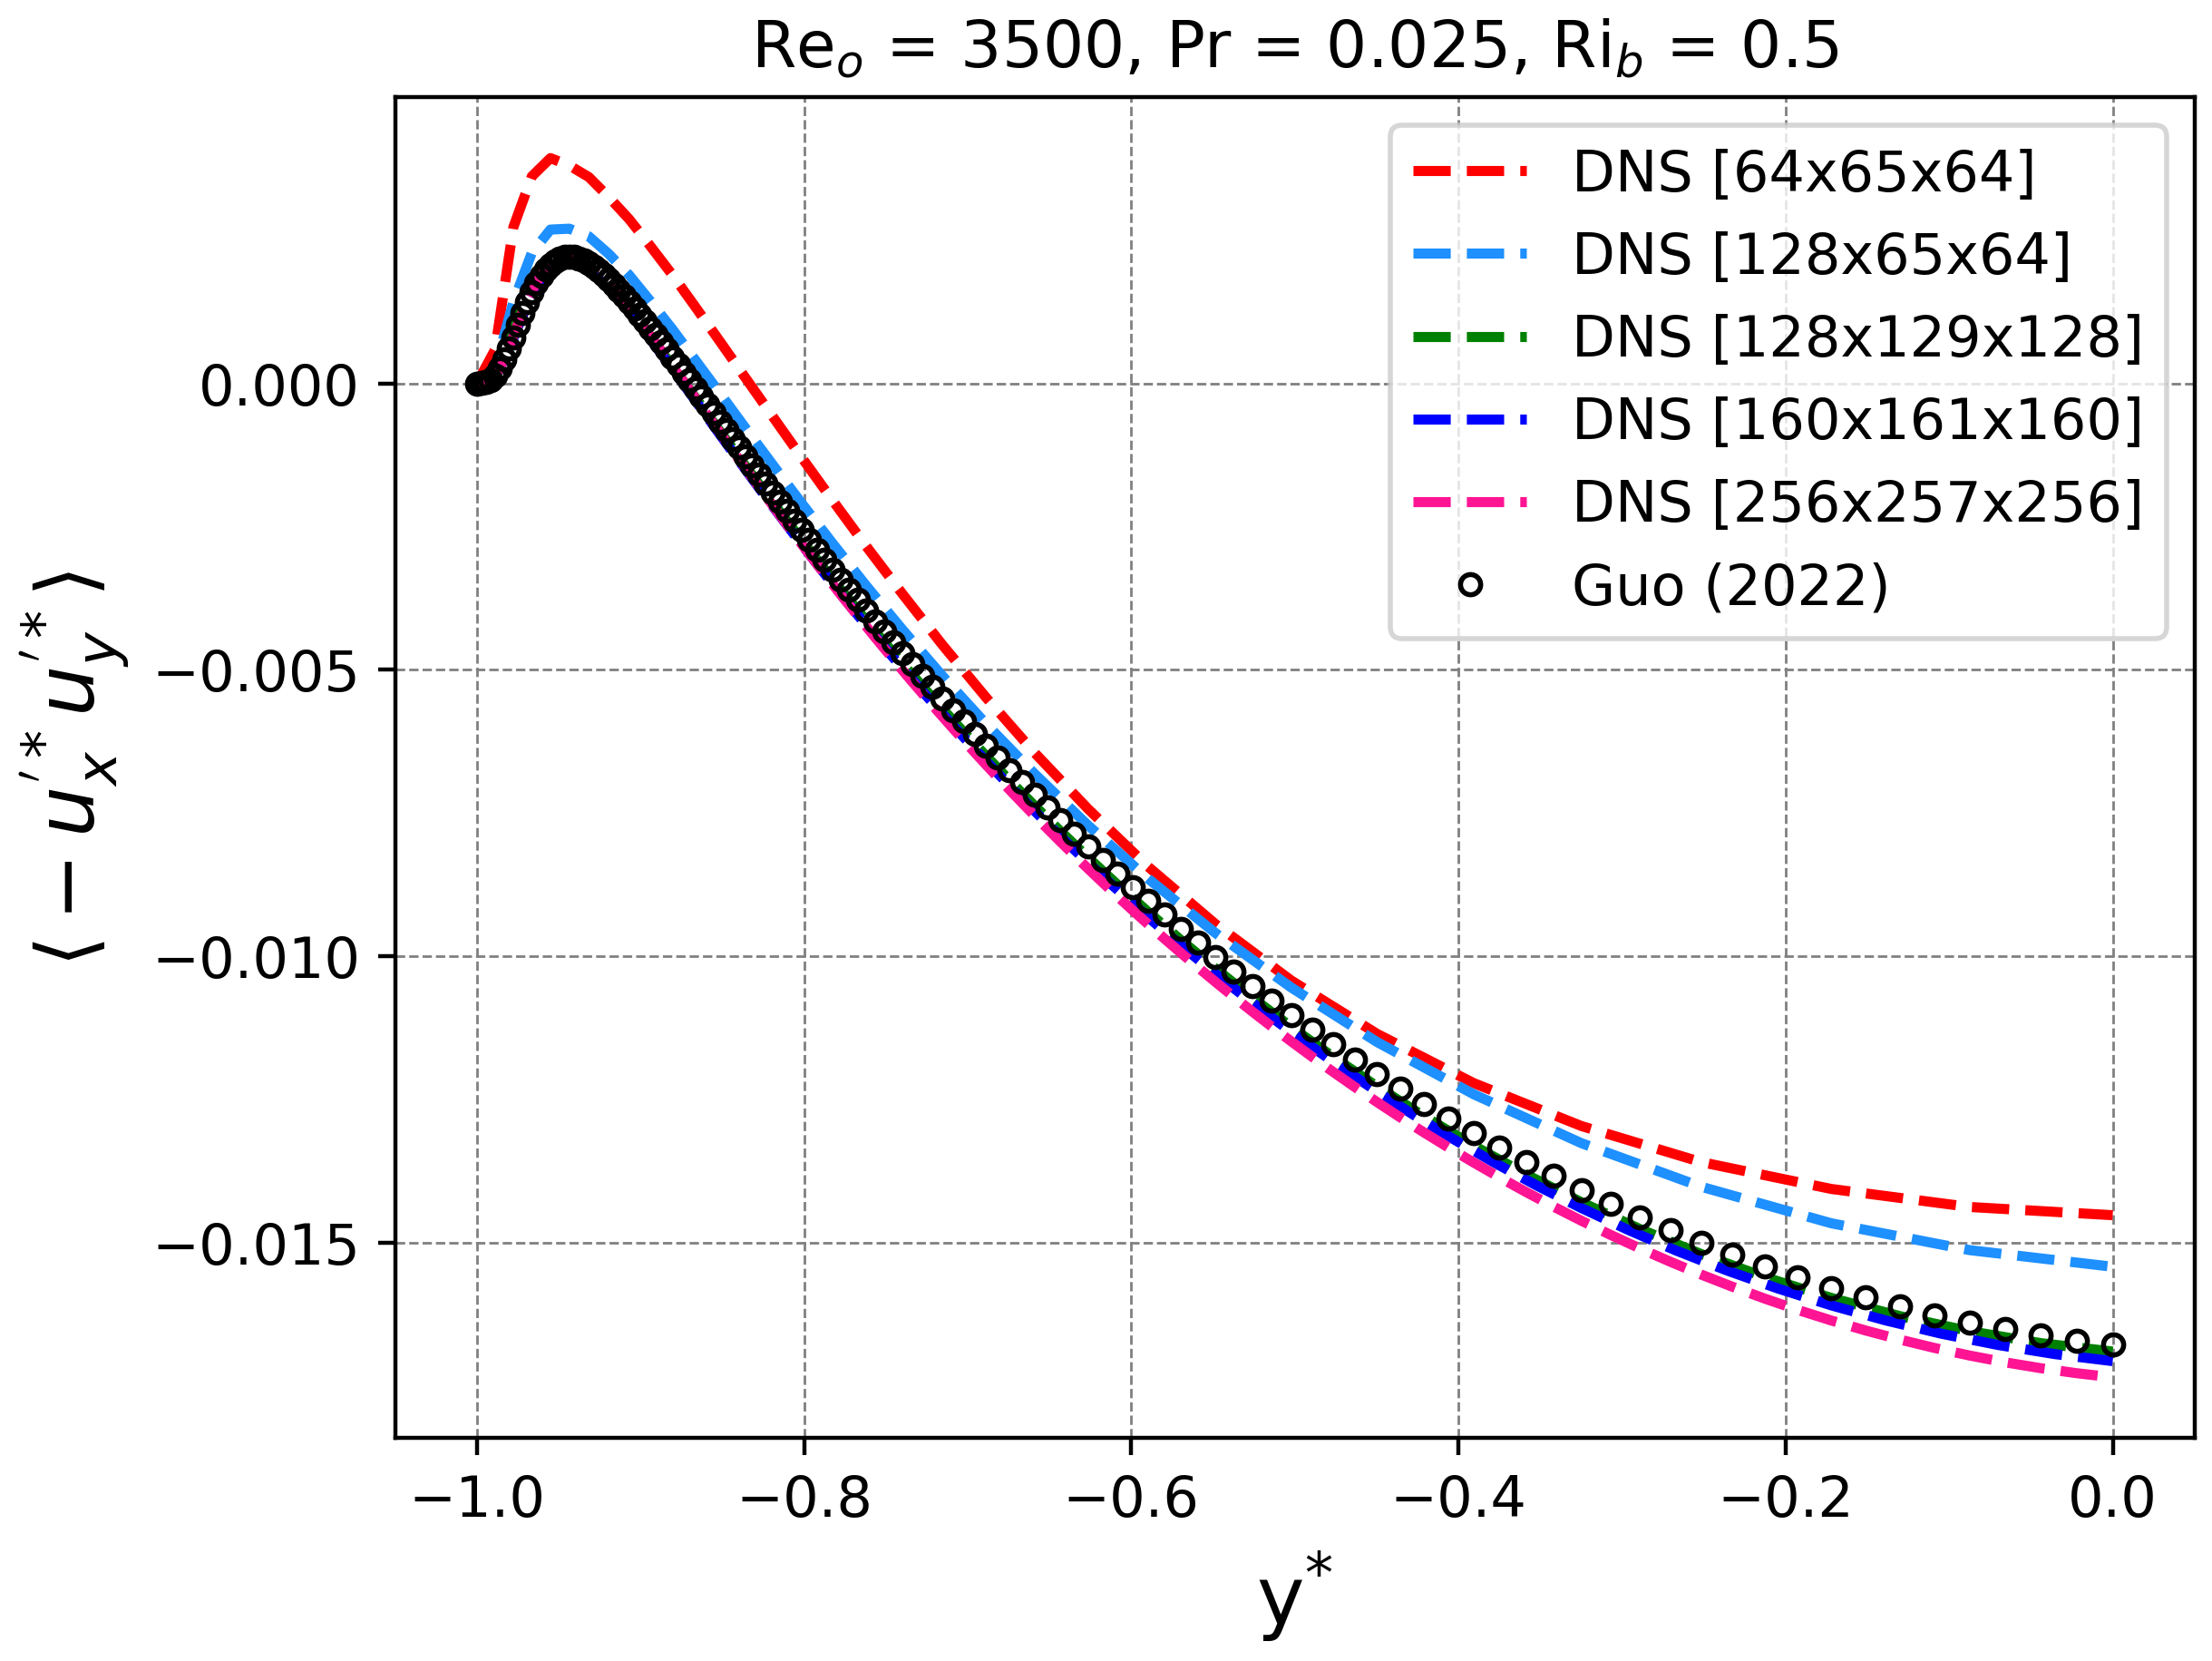
\includegraphics[width=0.49\textwidth]{figures/cap4/guo/Rib05/mct_up_vp.png}
    	\label{fig:guo-05-uxuy}}  
    \subfloat[]{
    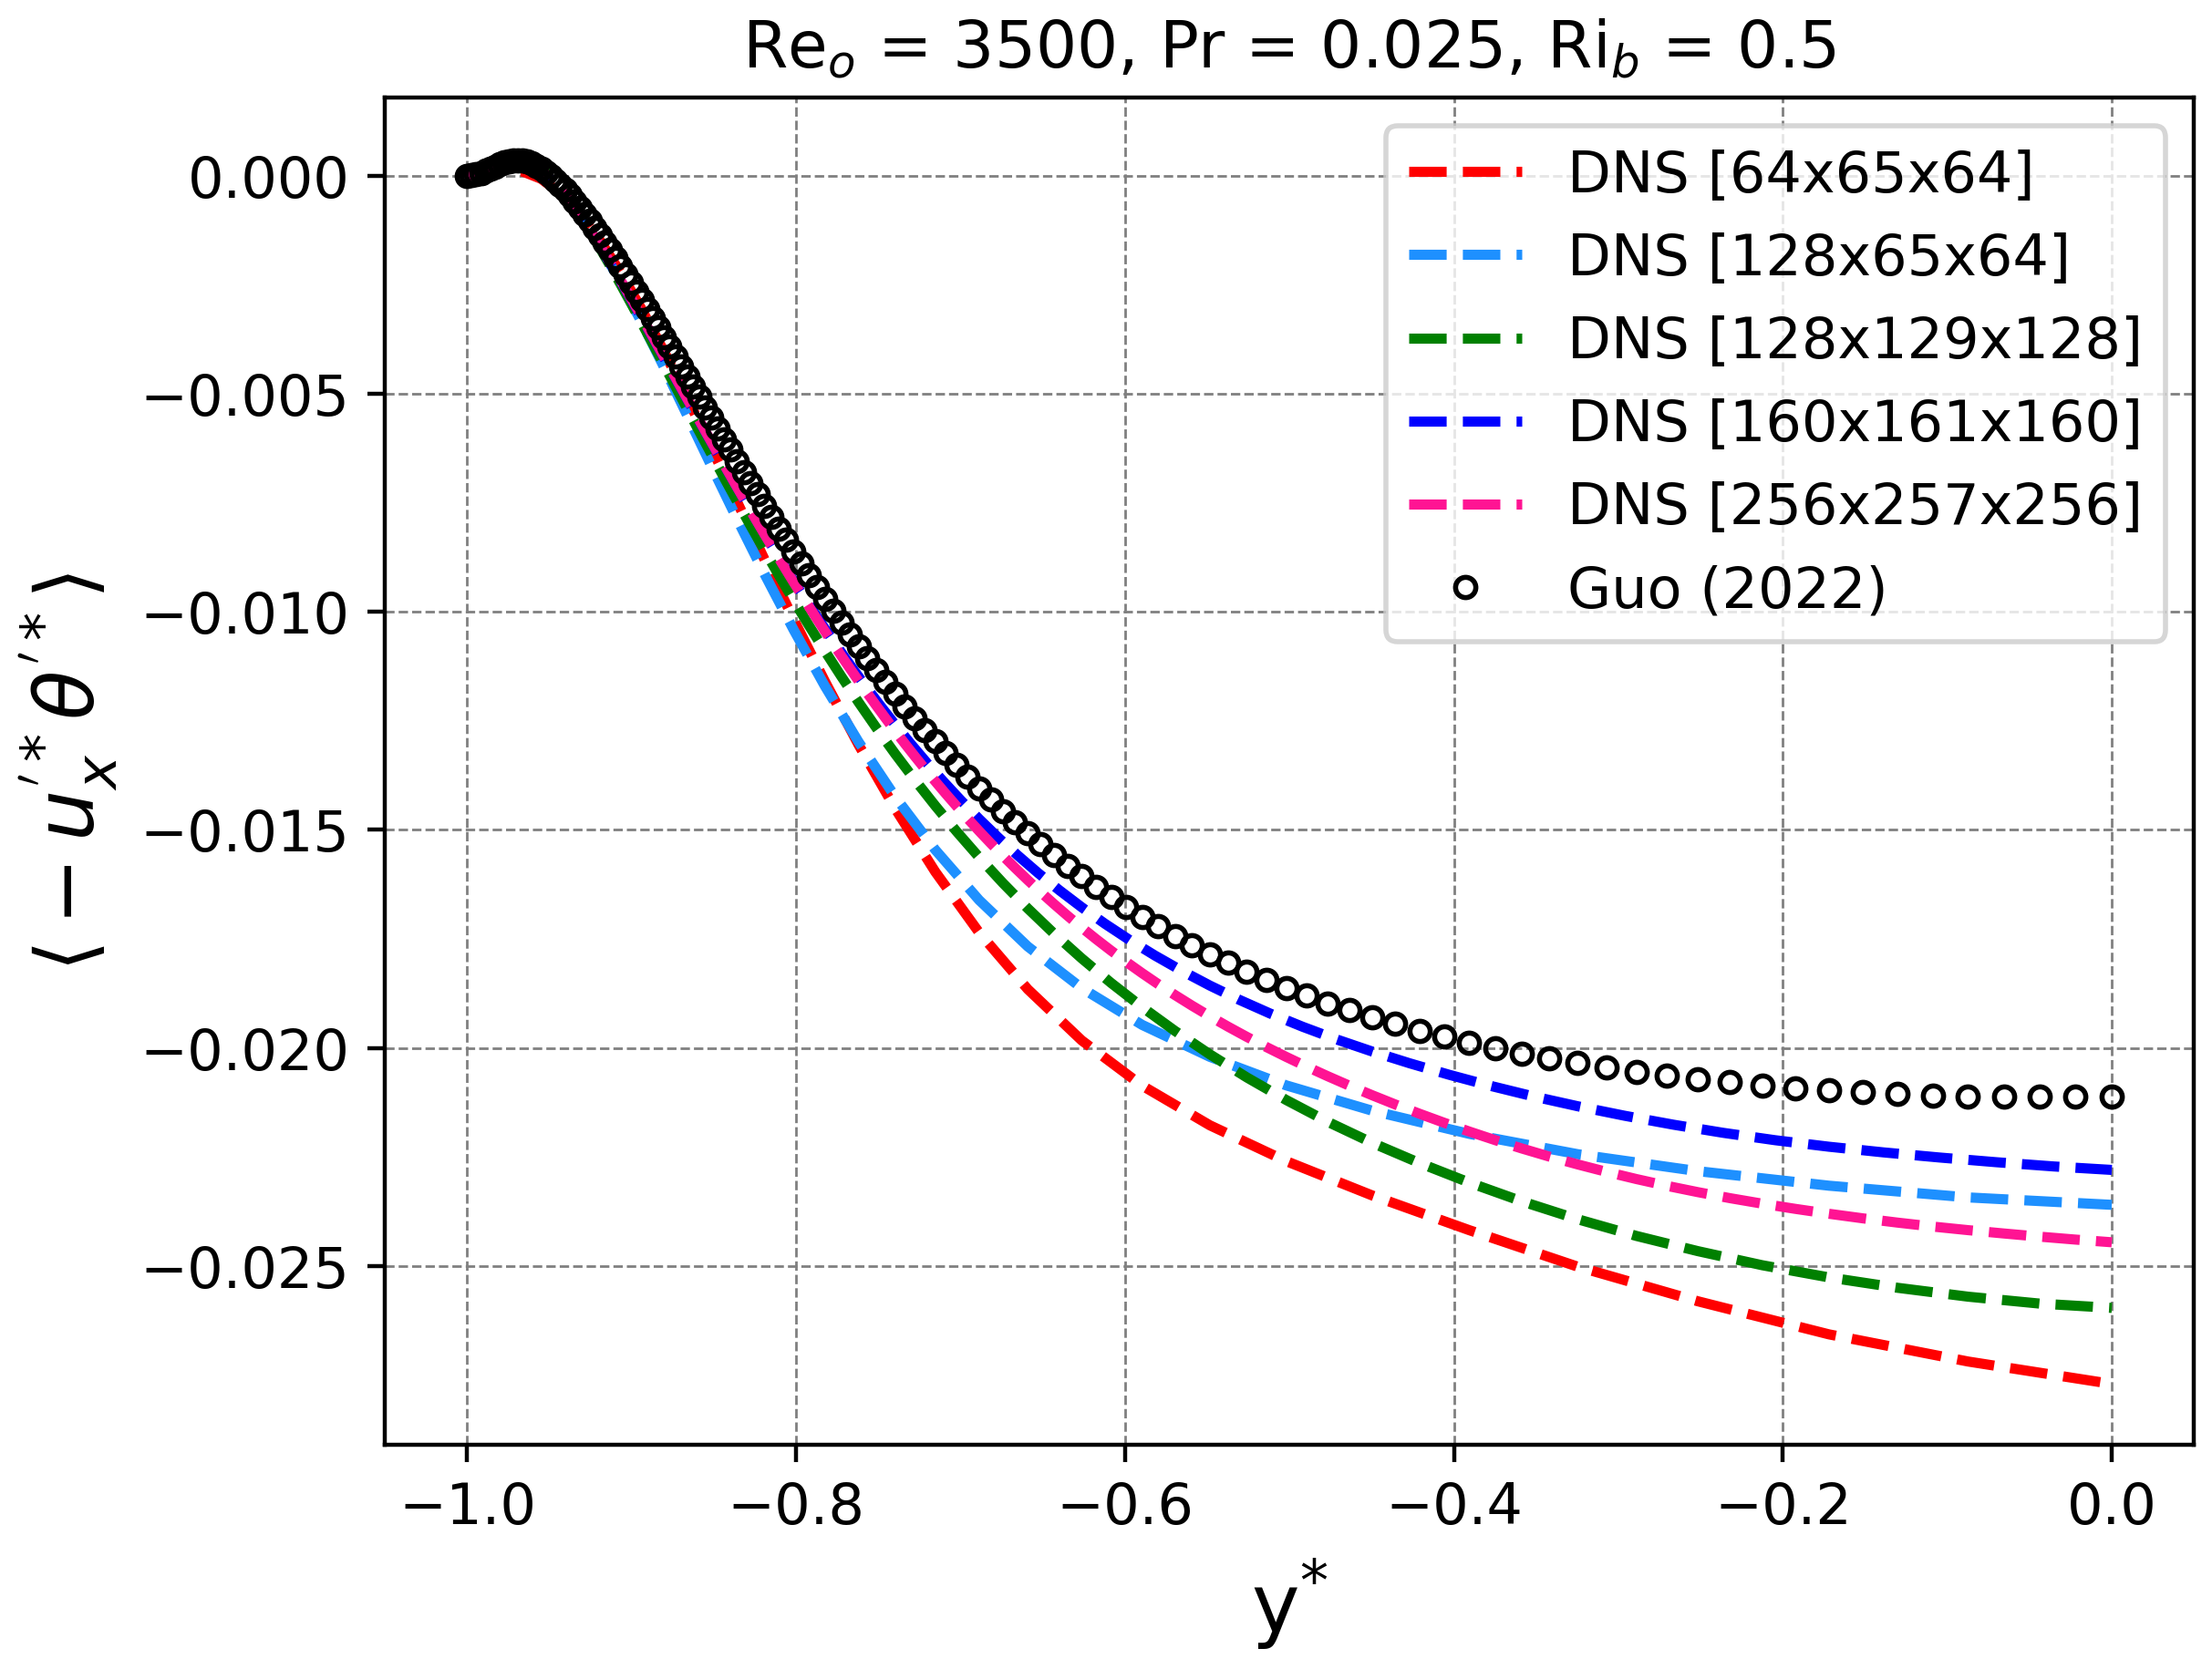
\includegraphics[width=0.49\textwidth]{figures/cap4/guo/Rib05/mct_up_thetap.png}
    	\label{fig:guo-05-ux-theta}}  
 \caption{Perfiles de \textbf{(a)} temperatura adimensional media, \textbf{(b)} fluctuaciones RMS de la temperatura adimensional, \textbf{(c)} velocidad media \textit{streamwise}, \textbf{(d)} fluctuaciones RMS de la velocidad \textit{streamwise}, \textbf{(e)} componente $xy$ del tensor de Reynolds, $\langle -u^+_x u^+_y \rangle$, y \textbf{(f)} flujo de calor turbulento en la dirección X, $\langle -u^+_x \theta^+ \rangle$.} 
 \label{fig:guo-05}
\end{figure}

Cuando se tiene en cuenta la fuerza boyante, es decir $\Pi \neq 0$, el término asociado a ella en la ecuación de momento produce un acople entre las ecuaciones de conservación de momento y energía (ecuaciones \ref{eq:gob_system_adim}) y por lo tanto, la parte hidrodinámica del flujo influye en la parte térmica del mismo y viceversa. 

Se realizan simulaciones empleando las mallas M0 - M4 para analizar su convergencia en malla. En este sentido, se consideran los números adimensionales Re$_o$=3500, Pr=0.025 y Ri$_b$=0.5 para tal fin. Las Figuras \ref{fig:guo-05-theta} - \ref{fig:guo-05-ux-theta} exponen, respectivamente, los perfiles de las siguientes magnitudes\footnote{Nótese que solo se representa un semiancho del canal, esto es, $-1 \leqslant y^* \leqslant 0$.}: temperatura adimensional, fluctuaciones de temperatura, velocidad \textit{streamwise}, fluctuaciones de velocidad, componente $xy$ del tensor de Reynolds y flujo de calor turbulento en la dirección $X$. Los datos de magnitudes propias se comparan con aquellos datos obtenidos por Guo \textit{et al.} \cite{guo2022direct}. Las mismas se encuentran expresadas en la forma adimensional: $\mathbf{u^*} = \mathbf{u} / U_b$ y $\theta^* = \theta / \Delta T_{hc}$, siendo $U_b$ la velocidad \textit{bulk} y $\Delta T_{hc}$ la diferencia de temperatura entre las paredes.

Se observa que las Figuras \ref{fig:guo-05-theta} y \ref{fig:guo-05-ux} verifican una buena convergencia en malla de las  magnitudes de primer orden, es decir, perfiles de velocidad media y temperatura media. Sin embargo, se puede identificar por simple observación, que las diferencias entre nuestras mallas M3 y M4 son, en algunas posiciones del canal, menores a las diferencias entre los datos de referencia y nuestros datos para M4. Esto sugiere que posteriores refinamientos no producirán soluciones más próximas a la referencia. 

Adicionalmente, al comparar magnitudes de segundo orden asociadas a la temperatura adimensional, como la fluctuación de temperatura (Figura \ref{fig:guo-05-theta-rms}) o el flujo de calor turbulento (Figura \ref{fig:guo-05-ux-theta}), se puede destacar una clara diferencia cuantitativa entre nuestros datos para M4 y la referencia en algunas posiciones del semiancho, como por ejemplo en el centro del canal. Por otro lado, en las magnitudes de segundo orden asociadas a la velocidad como las fluctuaciones (Figura \ref{fig:guo-05-ux-rms}) o la componente $xy$ de la tensión de Reynolds (Figura \ref{fig:guo-05-uxuy}), la discrepancia cuantitativa entre los datos obtenidos con M4 y aquellos de referencia sigue siendo apreciable en el centro del canal; sin embargo, es menor que la registrada para la temperatura.

Se especula que los aspectos más relevantes para explicar las diferencias encontradas en los perfiles de las magnitudes de segundo orden, están asociados al tamaño del dominio simulado. Guo \textit{et al.} utilizan un dominio ampliamente mayor ($L_x \times L_y \times L_z = 31\text{.}42 \times 2 \times 12\text{.}57$) que el empleado en este trabajo. Debido a la periodicidad en $x$, los puntos del plano medio $x = L_x/2$ están parcialmente influidos por los puntos en los planos $x=0$ y $x=L_x$. Dicho de otra manera, estos puntos ``fronterizos'' podrían no encontrarse descorrelacionados. Este hecho no permite capturar con presición todas las escalas que presenta la solución del problema o hace que la solución numérica aún sea dependiente del tamaño del dominio simulado. Otra cuestión adicional que puede influir, es que Guo \textit{et al.} emplean menor resolución (espaciado mayor) en las direcciones $X$ y $Z$, e idéntico en la dirección $Y$: $(\Delta x^*,\Delta y^*_{\text{max}},\Delta z^*) = (0\text{.}061, 0\text{.}022, 0\text{.}024)$. Por lo tanto, luego de esta discusión y del análisis de los resultados presentados en las Figuras \ref{fig:guo-05-theta} - \ref{fig:guo-05-ux-theta} se considera que las mallas propuestas, M2-M4, producen resultados con una precisión razonable para los objetivos buscados y permiten llevar adelante el trabajo con la capacidad de cálculo existente. 

\paragraph{Elección de malla para simulaciones posteriores.}

En síntesis, los resultados de esta sección muestran que refinar de M2 a M3/M4 no aporta mejoras apreciables a la escala de las figuras. Dado que las magnitudes de interés\footnote{Por ejemplo, el número de Nusselt y/o el factor de fricción de Darcy.} se obtienen a partir de cantidades estadísticas de primer orden, y además, estas mantienen un buen acuerdo con las referencias, \textbf{se adopta la malla M2} para las simulaciones del Capítulo \ref{cap:desarrollado} por representar el mejor compromiso entre precisión y costo computacional.


\section{Segunda Parte: OSMC}

En esta segunda parte se exponen los resultados obtenidos con la herramienta OSMC, la cual genera autovalores y autofunciones basados en teoría de estabilidad lineal presentada en el Capítulo \ref{cap:modelo}. La validación de la herramienta se realiza en dos etapas: 

\begin{itemize}
	\item \textbf{1.} se valida la fiabilidad de los autovalores calculados;
	\item \textbf{2.} se comparan autofunciones obtenidas con casos de referencia;
	%\item \textbf{3.} se realizan simulaciones DNS para un canal de placas paralelas, con flujo de calor constante en las paredes, cuya condición inicial se construye utilizando el autovalor más inestable y su autofunción asociada. Se compara su evolución temporal con aquella obtenida por análisis de estabilidad lineal.
\end{itemize}

\subsection{Autovalores}

Basados en el proyecto integrador de Pablo Szuban \cite{szuban2023}, se emplea la variación de la parte imaginaria del autovalor más inestable\footnote{Esto es: la parte imaginaria de la cota superior del espectro de autovalores calculado con OSMC para un determinado conjunto de parámetros $\lbrace \alpha, \beta, \text{Re}_o, \text{Pr}, \text{Ra} \rbrace$.}, $c_i$, en función del número de onda en la dirección $X$, $\alpha$, para validar los autovalores obtenidos con OSMC. La Figura \ref{fig:eigenval_alpha} muestra $c_i(\alpha)$ para $\mathrm{Re}_o=322$ y $\mathrm{Re}_o=750$, con $\beta=0$ y Pr = 0.7. Los valores de $\mathrm{Ra}$ se seleccionan de modo que $c_i=0$ para algún $\alpha$ dentro del intervalo considerado: $\mathrm{Ra}=32$.$65$ para \linebreak $\mathrm{Re}_o=322$ y $\mathrm{Ra}=37$.$6$ para $\mathrm{Re}_o=750$. Los resultados se comparan con los de Chen y \linebreak Chung \cite{chen1996linear}, observándose un muy buen acuerdo.

\begin{figure}[H]
	 \centering
    	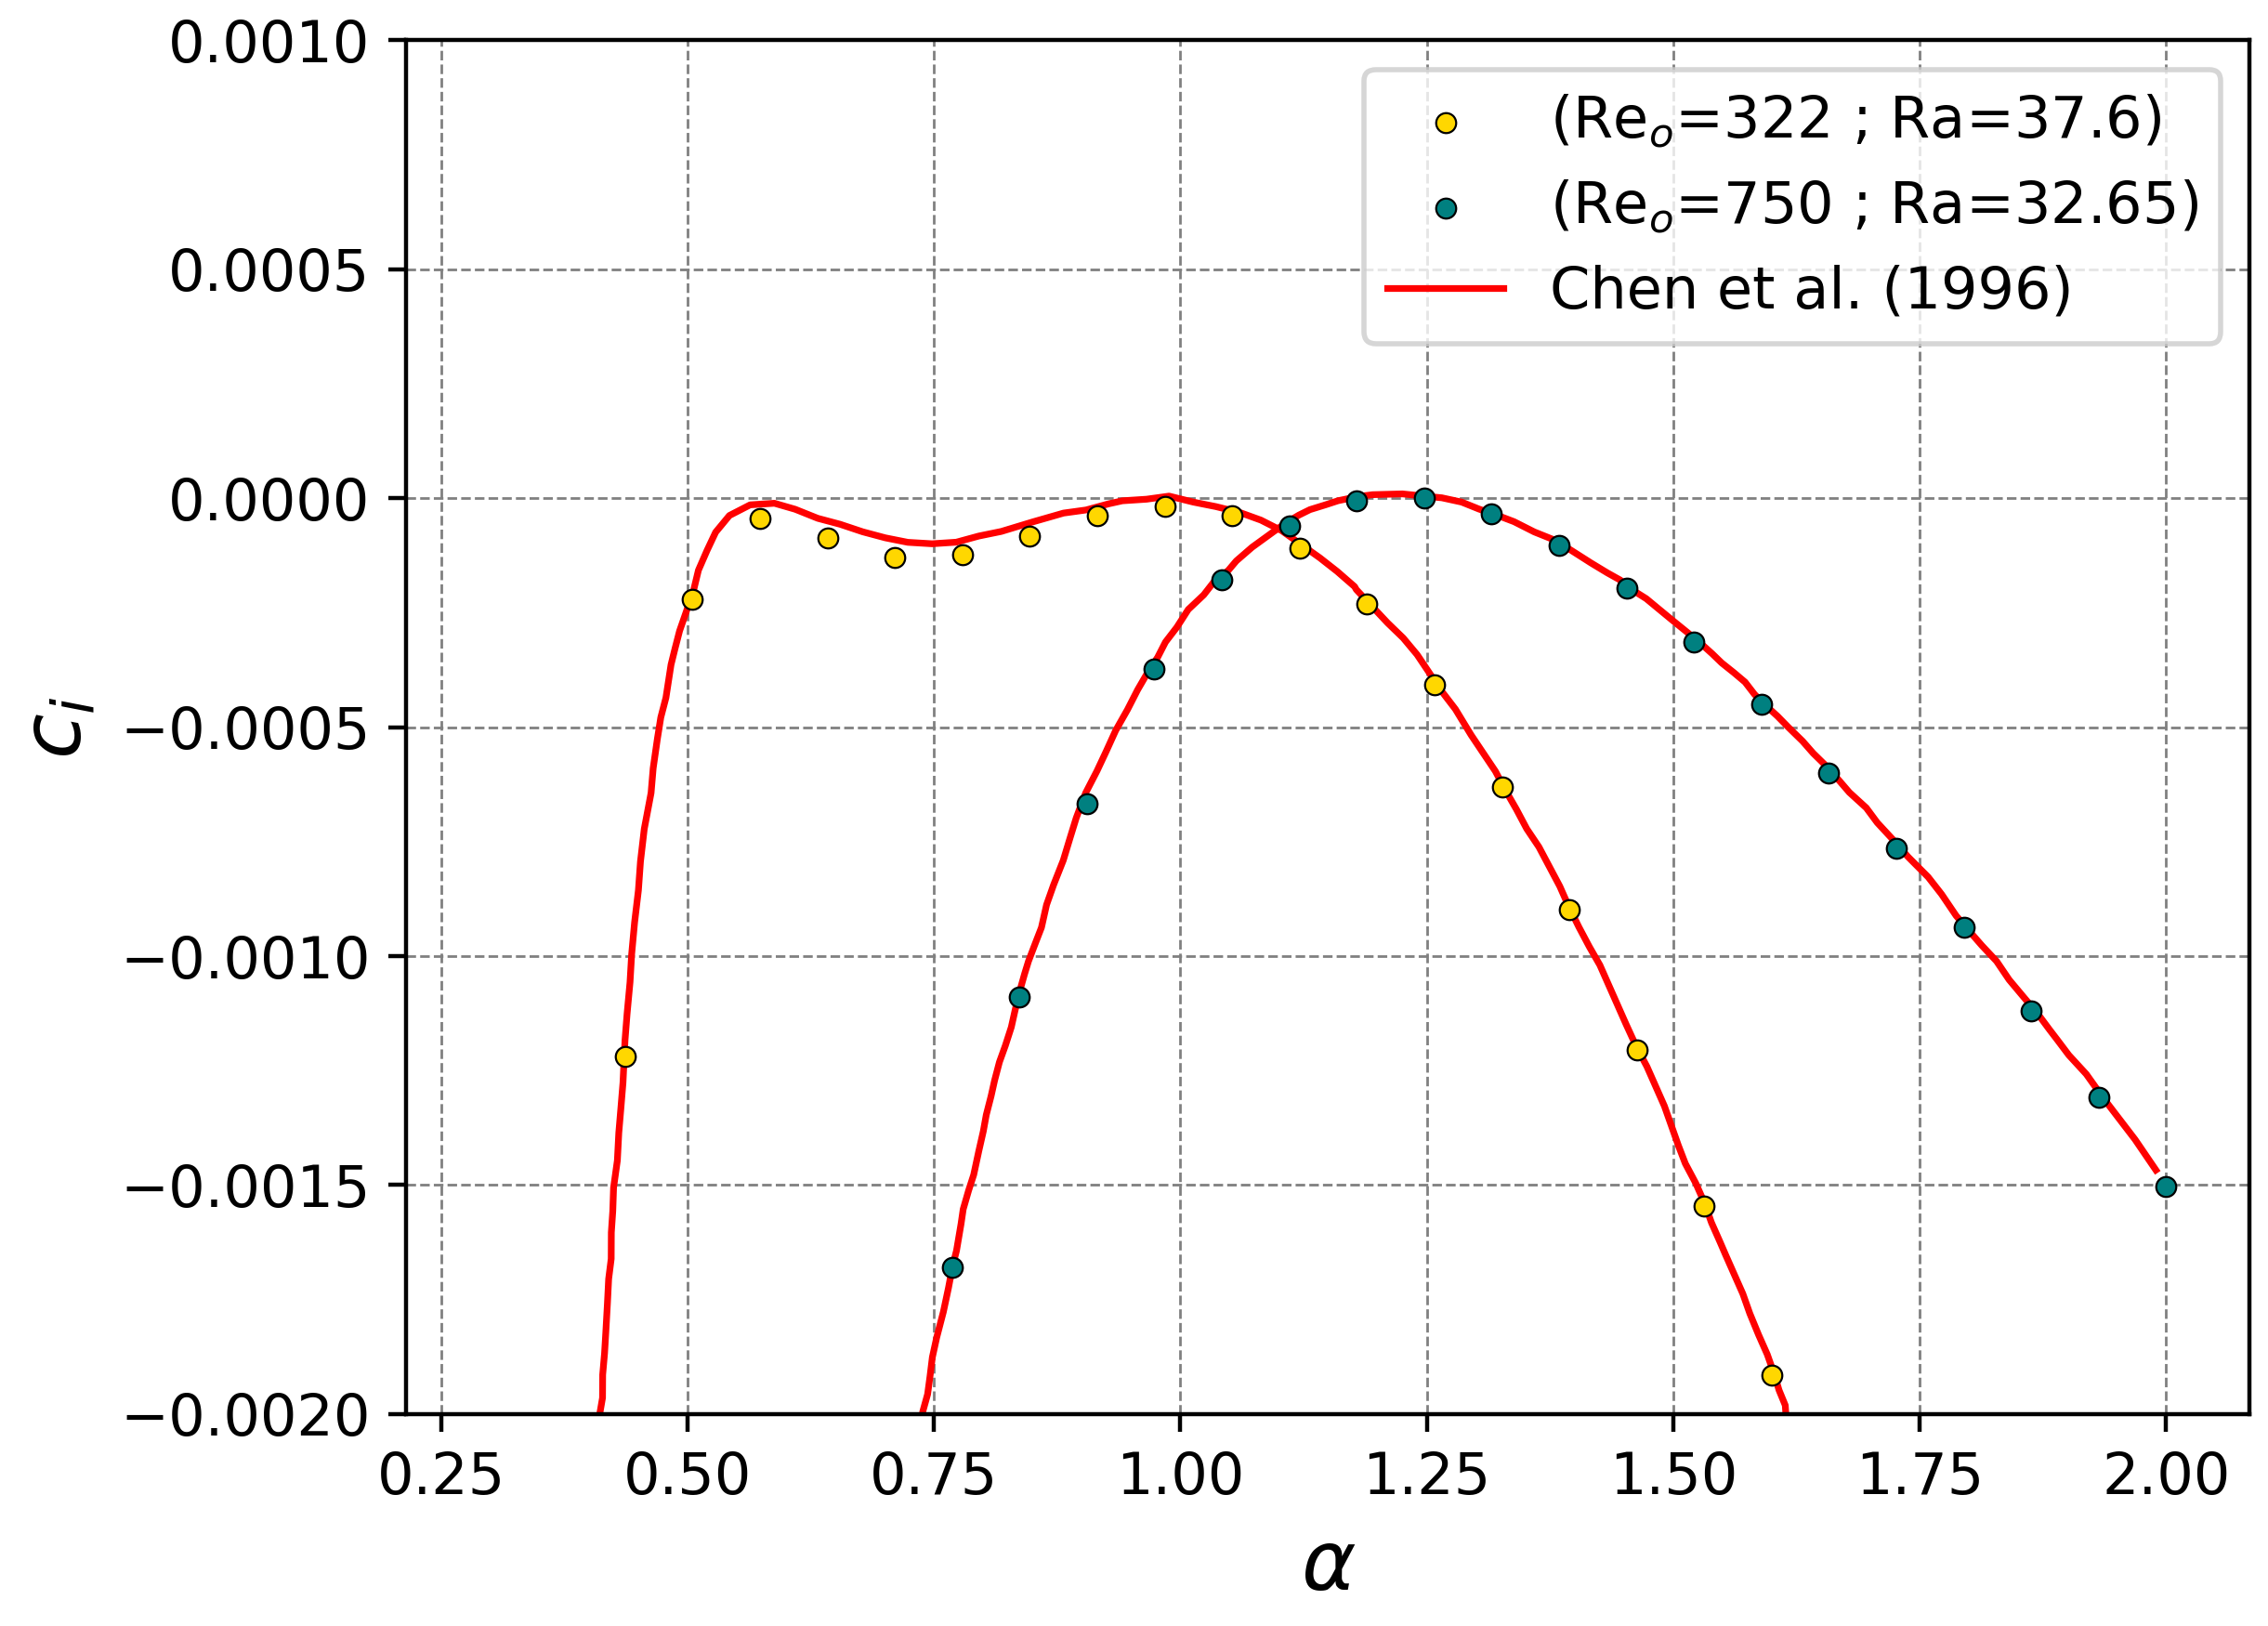
\includegraphics[width=0.6\textwidth]{figures/cap4/osmc/eigenvalues.png}
	 \caption{Variación de $c_i$ con $\alpha$ para diferentes valores de Re$_o$ con sus valores de Ra.} 
 \label{fig:eigenval_alpha}
\end{figure}


\subsection{Autofunciones}

\paragraph{Normalización.}
Sea $\{y_j\}_{j=1}^{N}$ la malla discreta en la dirección $Y$, las autofunciones \linebreak discretas $\{\widehat{v_x}(y_j),\widehat{v_y}(y_j),\widehat{v_z}(y_j),\widehat{\theta}(y_j)\}_{j=1}^{N}$ se normalizan localizando el índice donde el módulo de $\widehat{v_x}$ alcanza su valor máximo. Dicho índice se expresa de la siguiente forma:
$$
j_\star \;=\; \arg\max_{1\le j\le N}\,\big|\widehat{v_x}(y_j)\big|, 
\qquad 
\max_{1\le j\le N}\big|\widehat{v_x}(y_j)\big| \;=\; \big|\widehat{v_x}(y_{j_\star})\big|.
$$
Aquí, $\arg\max$ (argumento del máximo) denota el operador que devuelve el índice $j$ en el que la cantidad $|\widehat{v_x}(y_j)|$ alcanza su mayor valor. Luego, sea $u_\star=\widehat{v_x}(y_{j_\star})\neq 0$, se define un factor de normalización $c \in \mathbb{C}$ de forma tal que $\mathbb{R}\text{e}[c \, \widehat{v_x}(y_{j_\star})]=1$ y $\mathbb{I}\text{m}[c \, \widehat{v_x}(y_{j_\star})]=0$. A partir de estas dos condiciones se llega a que $c$ debe tener la forma:
$$
c \;:=\; \frac{\overline{u_\star}}{|u_\star|^2} \;=\; \frac{1}{u_\star}
$$
donde $\overline{(\text{.})}$ indica complejo conjugado. Con el mismo $c$ se escalan todas las autofunciones, para todo $j$, se tiene:
$$
\boldsymbol{\widehat{v}}_{\mathrm{norm}}(y_j)=c\,\boldsymbol{\widehat{v}}(y_j) \text{ ,} \quad
\widehat{\theta}_{\mathrm{norm}}(y_j)=c\,\widehat{\theta}(y_j).
$$
Nótese que si $u_\star=0$, la normalización anterior no aplica. Esta normalización es la empleada por Zang y Krist en su trabajo \cite{zang1989numerical} y es la que se utiliza por convención en la mayoría de la bibliografía.


En la Figura \ref{fig:eigenfun_valid} se presentan las autofunciones correspondientes al autovalor más inestable asociado a los parámetros $\text{Re}_o=1125$, $\text{Ra}=2500$ y Pr = 0.7. La Figura \ref{fig:eigenfun_2d} expone la autofunción de la velocidad \textit{streamwise} y de la temperatura para el caso de una onda 2D al considerar $\alpha=1$ y $\beta=0$. Por su parte, la Figura \ref{fig:eigenfun_3d} presenta las autofunciones de las mismas magnitudes para una onda 3D ahora considerando $\alpha=1$ y $\beta=1$. Ambos casos se comparan con las autofunciones calculadas por Chen y Chung \cite{chen2003direct}. Debe aclararse que los autores emplean una normalización distinta a la definida más arriba: cada una de las autofunciones $\left\lbrace \widehat{v_x}(y), \widehat{v_y}(y), \widehat{v_z}(y), \widehat{\theta}(y) \right\rbrace$ se normalizan por separado\footnote{Es decir, para cada autofunción considerada, se calcula una constante compleja $c$ diferente.} de modo que el máximo de la parte real sea igual a uno y su parte imaginaria sea nula. Al considerar esto y comparar las autofunciones obtenidas a partir de OSMC, con aquellos obtenidos por Chen y Chung, es posible apreciar un excelente acuerdo.

\newpage

\begin{figure}[H]
 \centering
  \subfloat[]{
    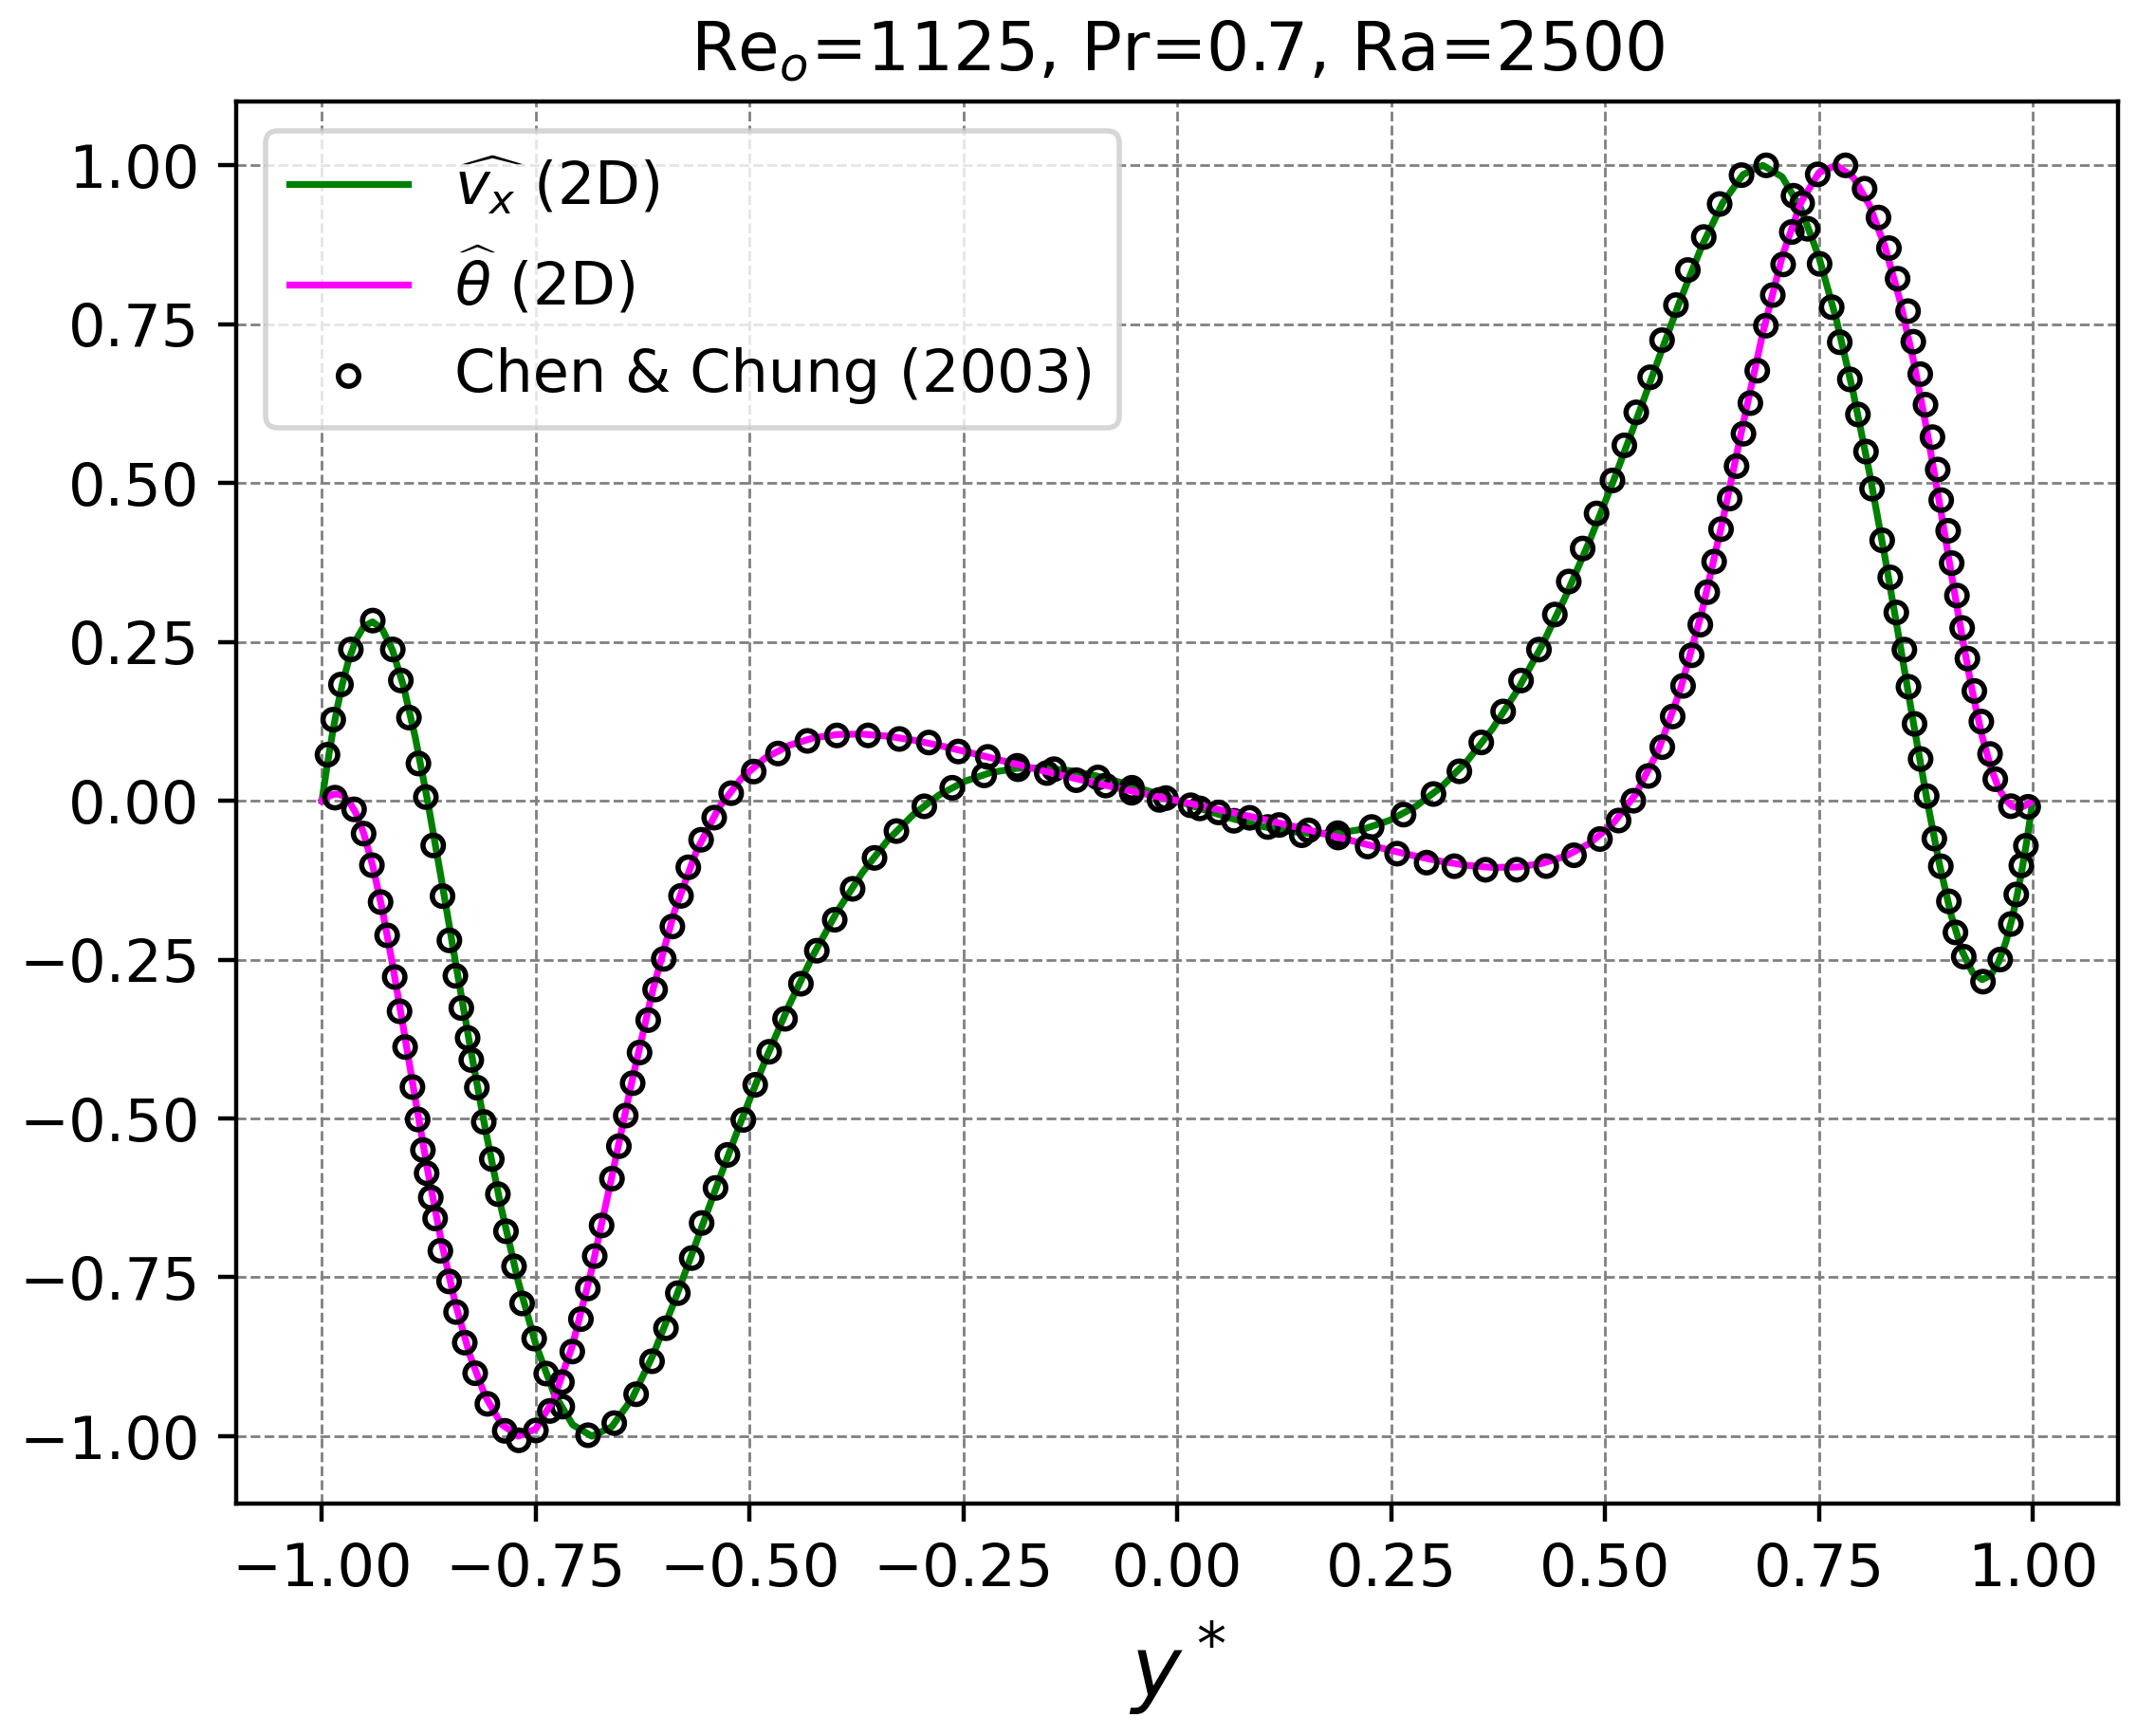
\includegraphics[width=0.49\textwidth]{figures/cap4/osmc/validation_eigenfuncs_2d.png}
    	\label{fig:eigenfun_2d}}  
    \subfloat[]{
    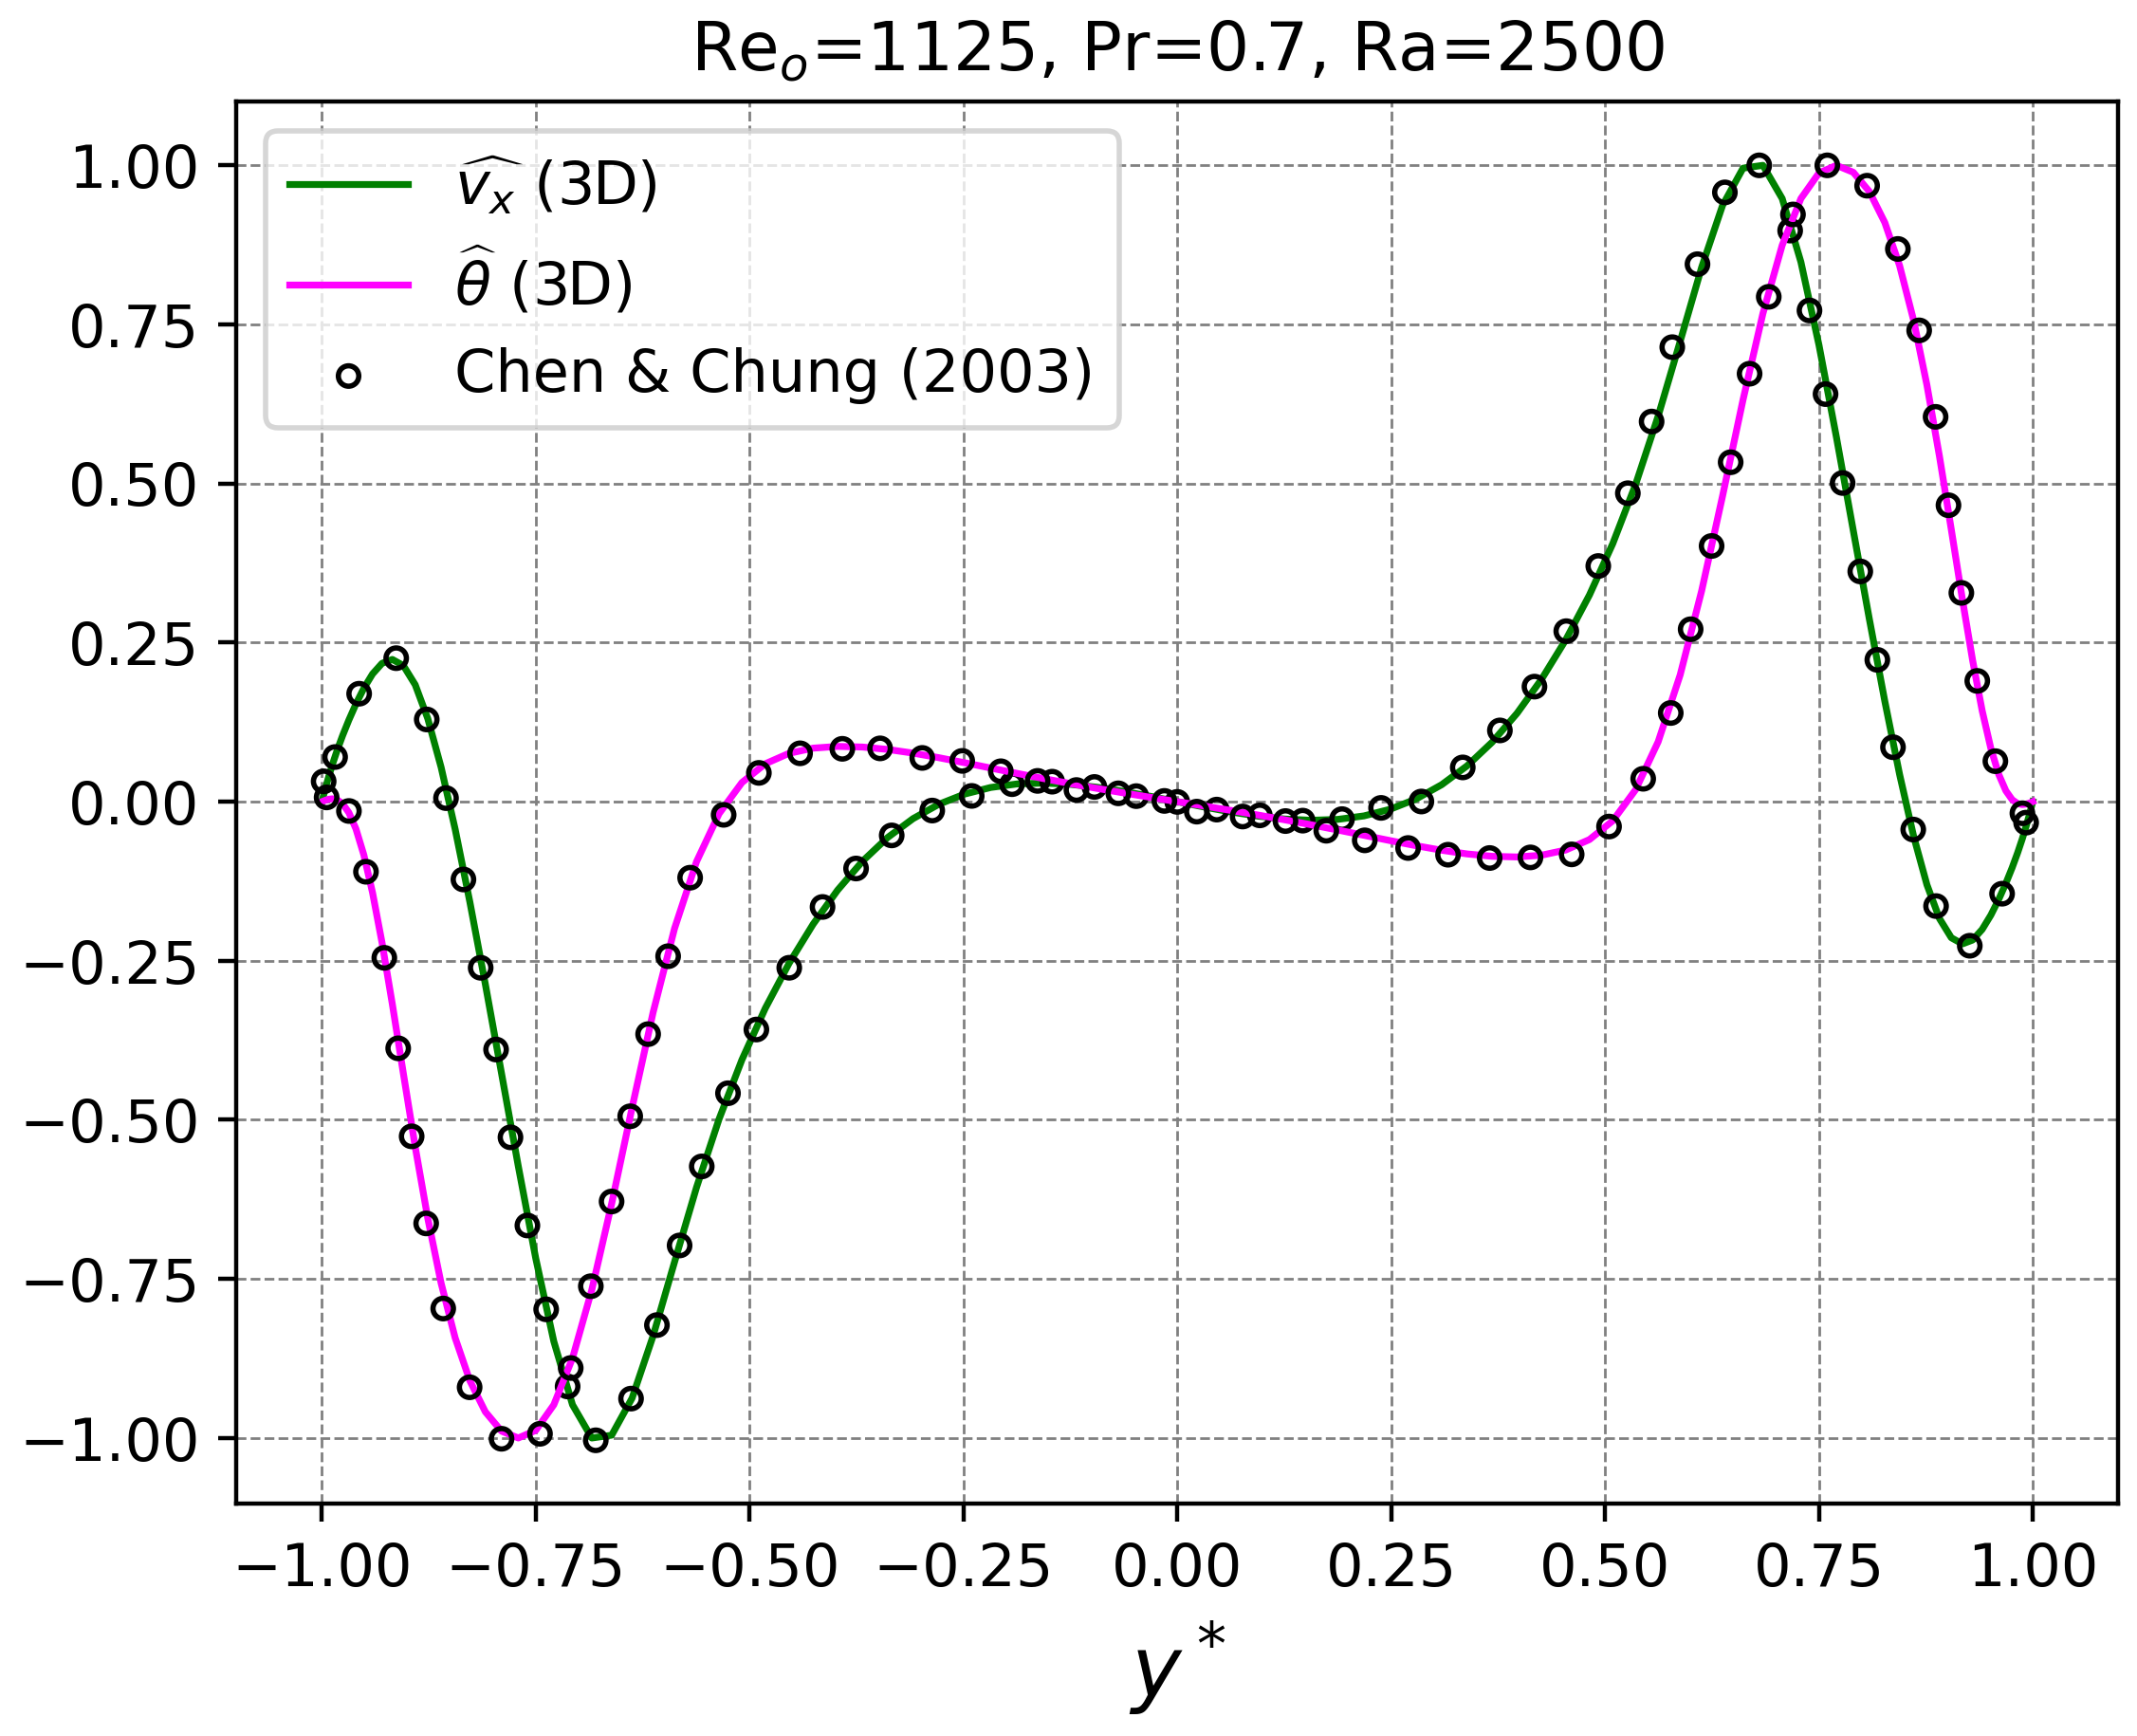
\includegraphics[width=0.49\textwidth]{figures/cap4/osmc/validation_eigenfuncs_3d.png}
    	\label{fig:eigenfun_3d}}  
 	\caption{Parte real de las autofunciones asociadas al modo más inestable para $\text{Re}_o=1125$, $\text{Ra}=2500$ y Pr = 0.7; \textbf{(a)} Onda 2D con ($\alpha$,$\beta$) = (1,0) y \textbf{(b)} Onda 3D con ($\alpha$,$\beta$) = (1,1).} 
 \label{fig:eigenfun_valid}
\end{figure}

\section{Análisis de Estabilidad Lineal versus DNS}

Como se menciona en la Sección \ref{line_an}, el análisis de estabilidad lineal predice a través de un modelo matemático la evolución temporal de pequeñas perturbaciones que son impuestas al flujo base. En esta sección, se realizan simulaciones DNS para un canal de placas paralelas, con flujo de calor constante en las paredes, cuya condición inicial se construye utilizando el autovalor más inestable y su autofunción asociada. En ese sentido, se pretende comparar las predicciones teóricas con los resultados arrojados por simulaciones realizadas con XC3D. Esto se realiza en escalas de tiempo donde las perturbaciones se mantienen relativamente acotadas (lo que hace válida a la aproximación del modelo lineal). Las condiciones iniciales de la simulación se construyen como la suma del flujo laminar, ecuaciones \ref{eq:vel_asist_boyant} - \ref{eq:theta_opo_boyant}, y las perturbaciones \ref{eq:init_con_1} - \ref{eq:init_con_3}. 

Se comparan dos casos, denominados\footnote{Nótese que Rama Izquiera y Rama Derecha hacen referencia a las ``ramas'' o ``brazos'' del espectro de autovalores considerado (véase Figura \ref{fig:Ra65RD-2d} y/o \ref{fig:Ra65RI-2d}).} Rama Izquierda (RI) y Rama Derecha (RD), que corresponden a casos físicos donde se incrementa y se disminuye la amplitud de la perturbacion inicial, respectivamente. Esto, matemáticamente, equivale a una parte imaginaria negativa (RI) y positiva (RD). Los números adimensionales empleados corresponden a $\text{Re}_o=750$, $\text{Pr}=0\text{.}7$ y $\text{Ra}=65$. Los parámetros de simulación de ambos casos se exponen en la \linebreak Tabla \ref{tab:caseslineal-theor}. Obsérvese que se utilizan perturbaciones compuestas únicamente de ondas bidimensionales. Las Figuras \ref{fig:Ra65RD-2d} (RD) y \ref{fig:Ra65RI-2d} (RI) muestran, de izquierda a derecha: (i) el espectro de autovalores (puntos celestes) con el autovalor seleccionado (punto rojo); (ii) las autofunciones de las componentes de la velocidad; y (iii) la autofunción de la temperatura. Las simulaciones DNS realizadas se corren un total de 20 unidades temporales.

\begin{table}[H]
\centering
\resizebox{\textwidth}{!}{%
\begin{tabular}{lccccccccc}
\toprule
Caso & L$_x \times$ L$_y \times$ L$_z$ & N$_x \times$ N$_y \times$ N$_z$ & $\Delta t^*$ & $\alpha$ & $\beta$ & A$_{2D}$ & A$_{3D}$ & $c_{2D}$ \\
\midrule
RI & $2 \pi / \alpha \times 2 \times 2 \pi $ & $160 \times 161 \times 160$ & 0.001 & 1.22 & 0 & 0.2 \% & 0 \% & 0.656 - 0.0237 j \\
RD & $2 \pi / \alpha \times 2 \times 2 \pi $ & $160 \times 161 \times 160$ & 0.001 & 1.22 & 0 & 0.2 \% & 0 \% & 1.239 + 0.042 j \\
\bottomrule
\end{tabular}}
\caption{Parámetros de simulación de los dos casos elegidos.}
\label{tab:caseslineal-theor}
\end{table}

\begin{figure}[H]
 \centering 
  \subfloat[]{
    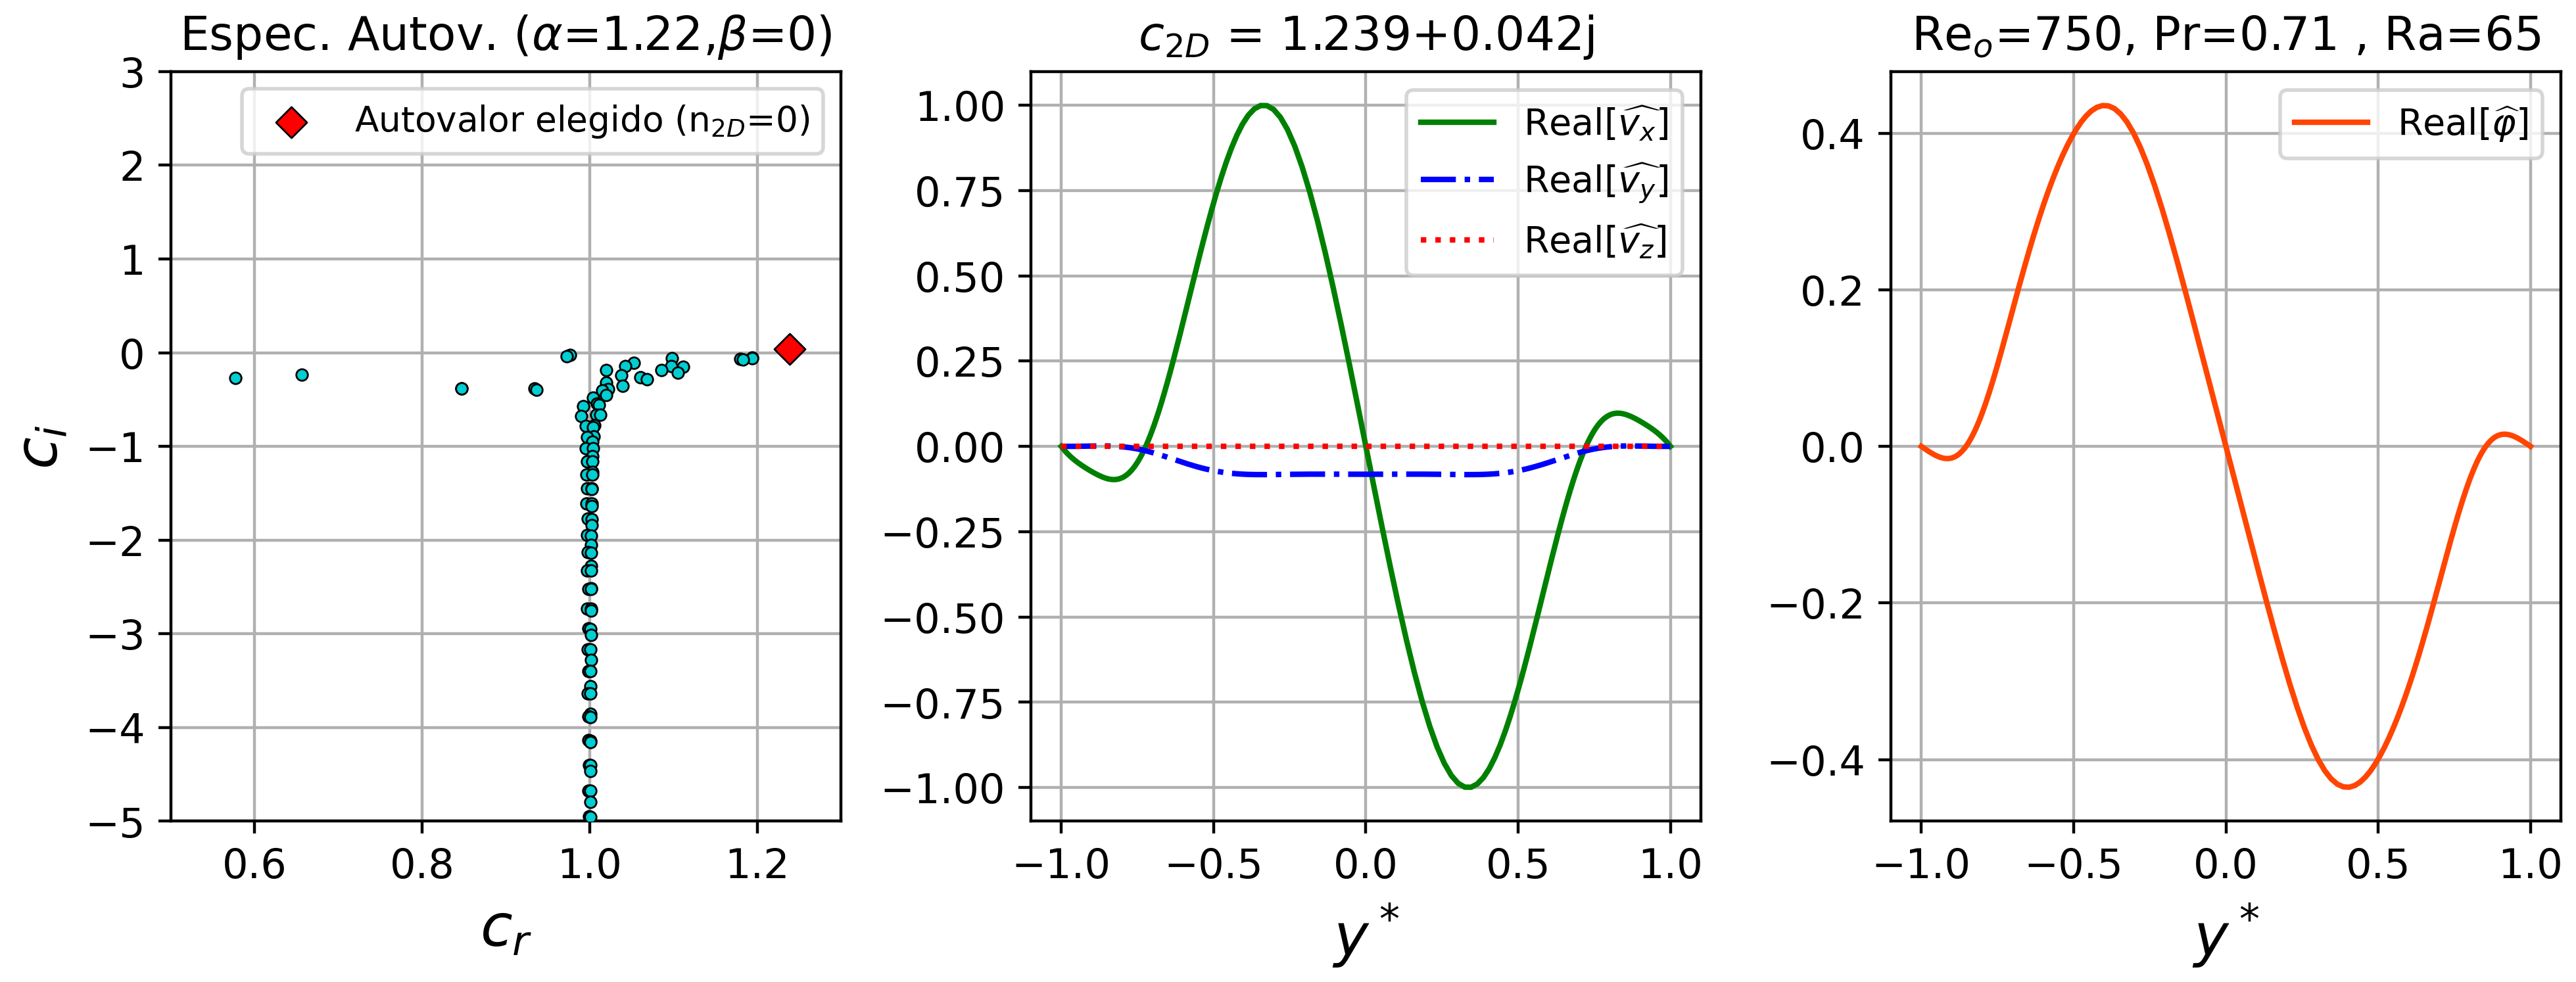
\includegraphics[width=0.8\textwidth]{figures/cap4/osmc/Ra65_RamaDer/2d_eigenfun.png}
    \label{fig:Ra65RD-2d}}
      
    \subfloat[]{
    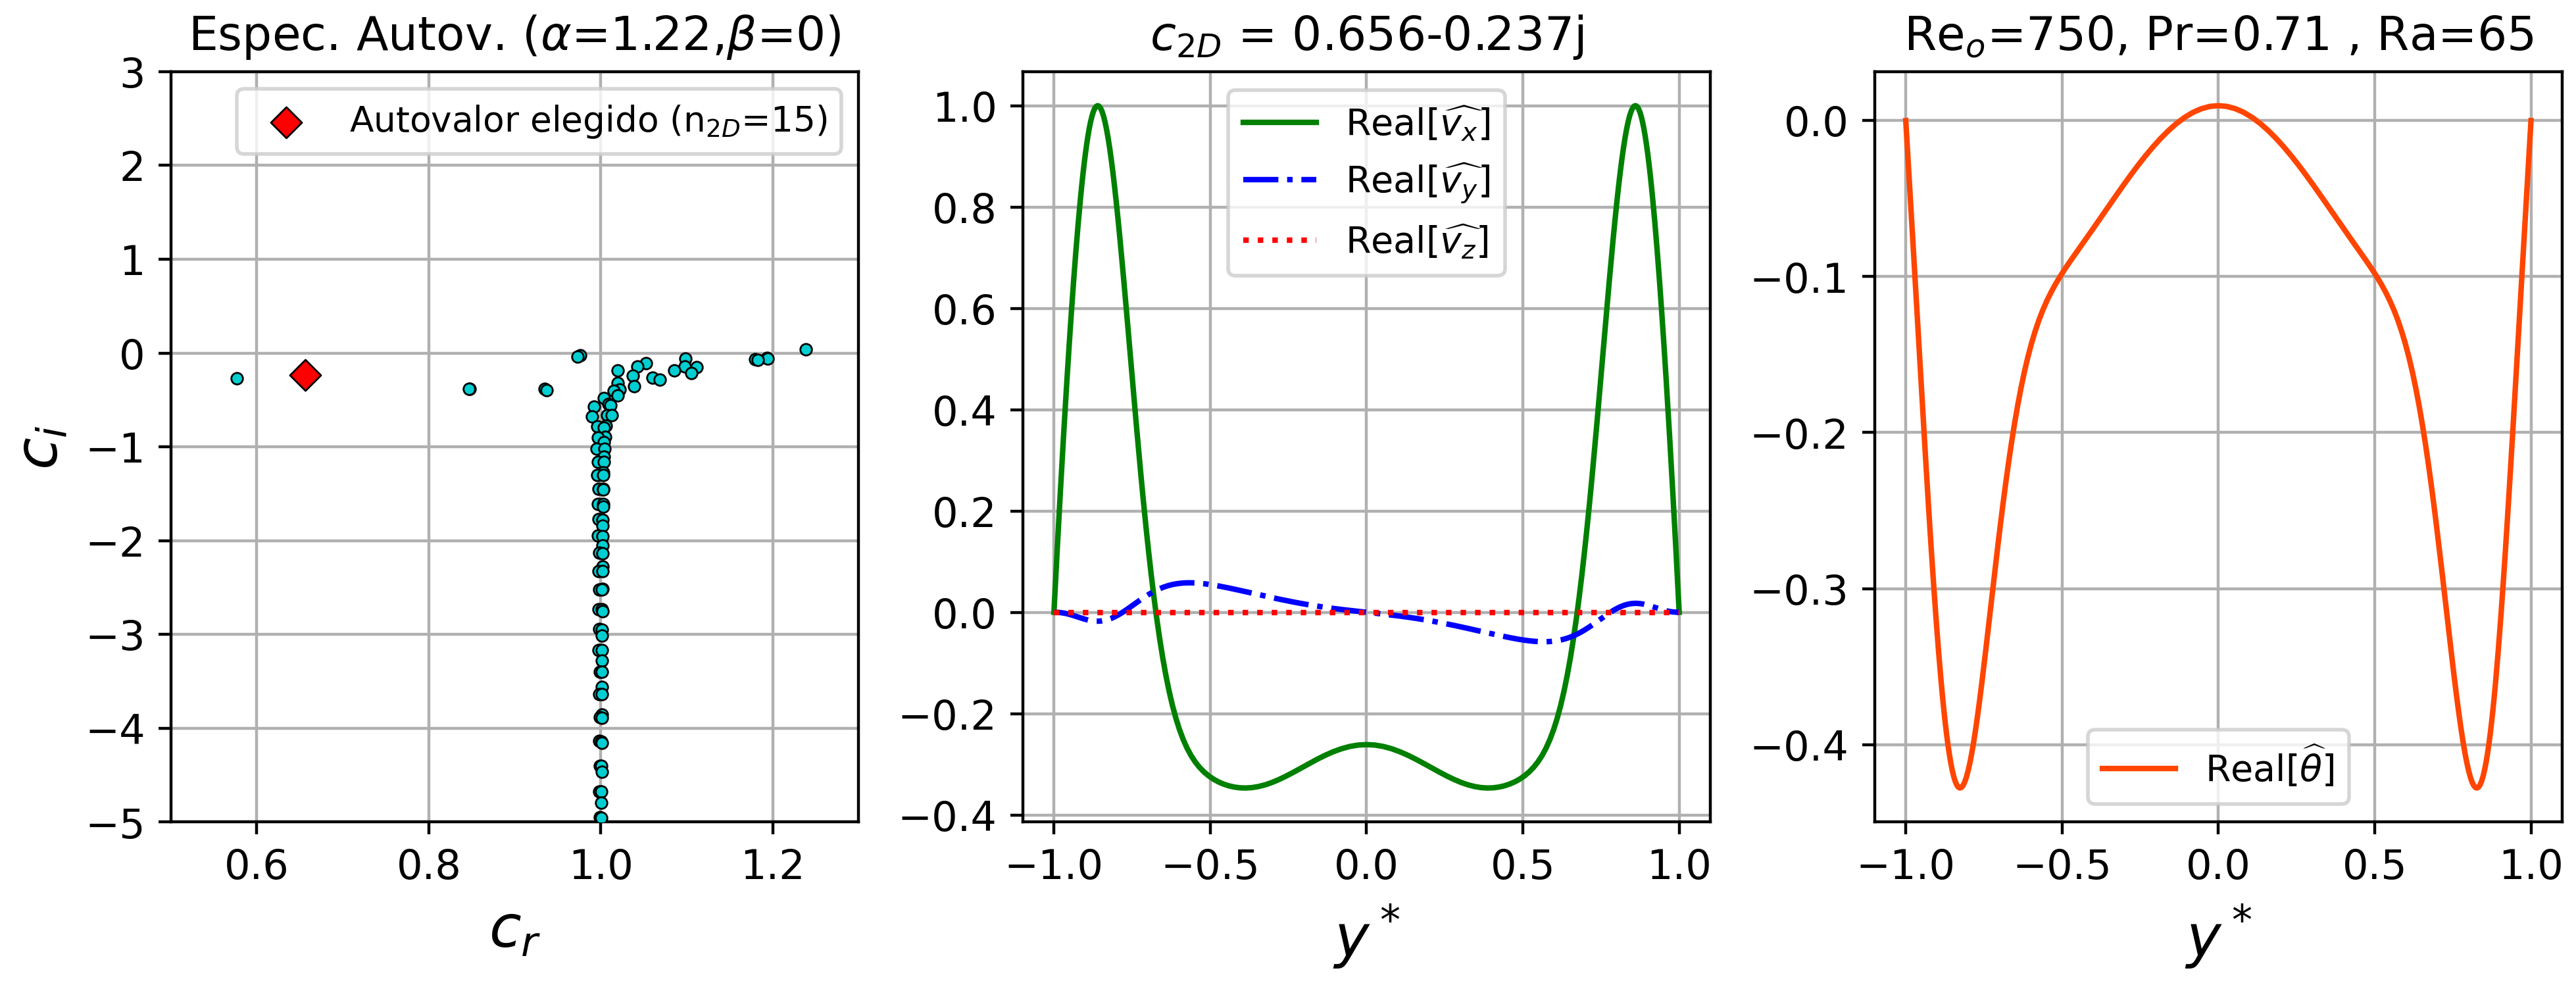
\includegraphics[width=0.8\textwidth]{figures/cap4/osmc/Ra65_RamaIzq/2d_eigenfun.png}
    \label{fig:Ra65RI-2d}}  
 \caption{De izquierda a derecha: (i) espectro de autovalores (puntos celestes) con el autovalor seleccionado (punto rojo); (ii) autofunciones de las componentes de la velocidad; (iii) autofunción asociada a la temperatura. \textbf{(a)} Caso RD y \textbf{(b)} Caso RI.} 
 \label{fig:Ra65-2d}
\end{figure}



Para comprobar la predicción de la teoría de estabilidad lineal con aquella producida por las herramientas numéricas, se emplea la evolución temporal de la energía cinética turbulenta (TKE) y de la varianza de la temperatura. En XC3D, dichas magnitudes corresponden al promedio integral en $y^*$ de las correlaciones $( \langle u^{* \prime}_x u^{* \prime}_x \rangle + \langle u^{* \prime}_y u^{* \prime}_y  \rangle + \langle u^{* \prime}_z u^{* \prime}_z  \rangle) / 2$ y $\langle \theta^{* \prime} \theta^{* \prime} \rangle$. En teoría de estabilidad lineal dichas cantidades se aproximan utilizando las autofunciones $\left\lbrace \widehat{v_x}, \widehat{v_y}, \widehat{v_z}, \widehat{\theta} \right\rbrace$ y las expresiones tipo \ref{eq:waves3d} para obtener:
\begin{align}
\text{TKE} &\simeq \frac{1}{2} (A_{2D})^2 \hspace*{0.5mm} e^{2 \alpha c_i t^*} \int \left[  ( \widehat{v_x}, \widehat{v_y}, \widehat{v_z} ) \cdot ( \widehat{v_x}, \widehat{v_y}, \widehat{v_z} )  \right] dy^* \text{ ,} \\
\int \langle \theta^{* \prime} \theta^{* \prime} \rangle dy^* &\simeq \frac{1}{2} (A_{2D})^2 \hspace*{0.5mm} e^{2 \alpha c_i t^*} \int (\widehat{\theta})^2 dy^* \text{ .}
\end{align}   
En estas expresiones, si $c_i < 0$, las cantidades decaen y el flujo es estable. Pero por el contrario, si $c_i > 0$, las mismas crecen y el flujo base evoluciona en el tiempo, dando posiblemente, origen a la transición. Las afirmaciones anteriores son ciertas siempre que $\alpha$ sea positivo.

Las Figuras \ref{fig:Ra65RD-tke} y \ref{fig:Ra65RD-tvar} muestran la evolución temporal de la TKE y de la varianza de la temperatura para el caso RD. Se observa un muy buen acuerdo entre la predicción teórica y los resultados obtenidos a partir de simulaciones DNS con las herramientas numéricas utilizadas. En este caso se aprecia que la perturbación introducida logra inestabilizar el flujo (pues $c_i>0$) y que si bien en una etapa temprana el acuerdo entre ambas metodologías coincide, si el flujo transiciona a un régimen turbulento, la consistencia entre ambos debería tender a desaparecer.  

De forma completamente análoga, las Figuras \ref{fig:Ra65RI-tke} y \ref{fig:Ra65RI-tvar} muestran la evolución temporal de la TKE y de la varianza de la temperatura para el caso RI. En este caso, dado que $c_i<0$, el análisis de estabilidad lineal predice que la perturbación impuesta tenderá a decaer y el flujo no se inestabilizará. Esta predicción está en completa consistencia con la simulación DNS realizada. Esto nos permite confirmar que la implementación de la condición inicial perturbada en XC3D es correcta.  

\begin{figure}[H]
 \centering
  \subfloat[]{
    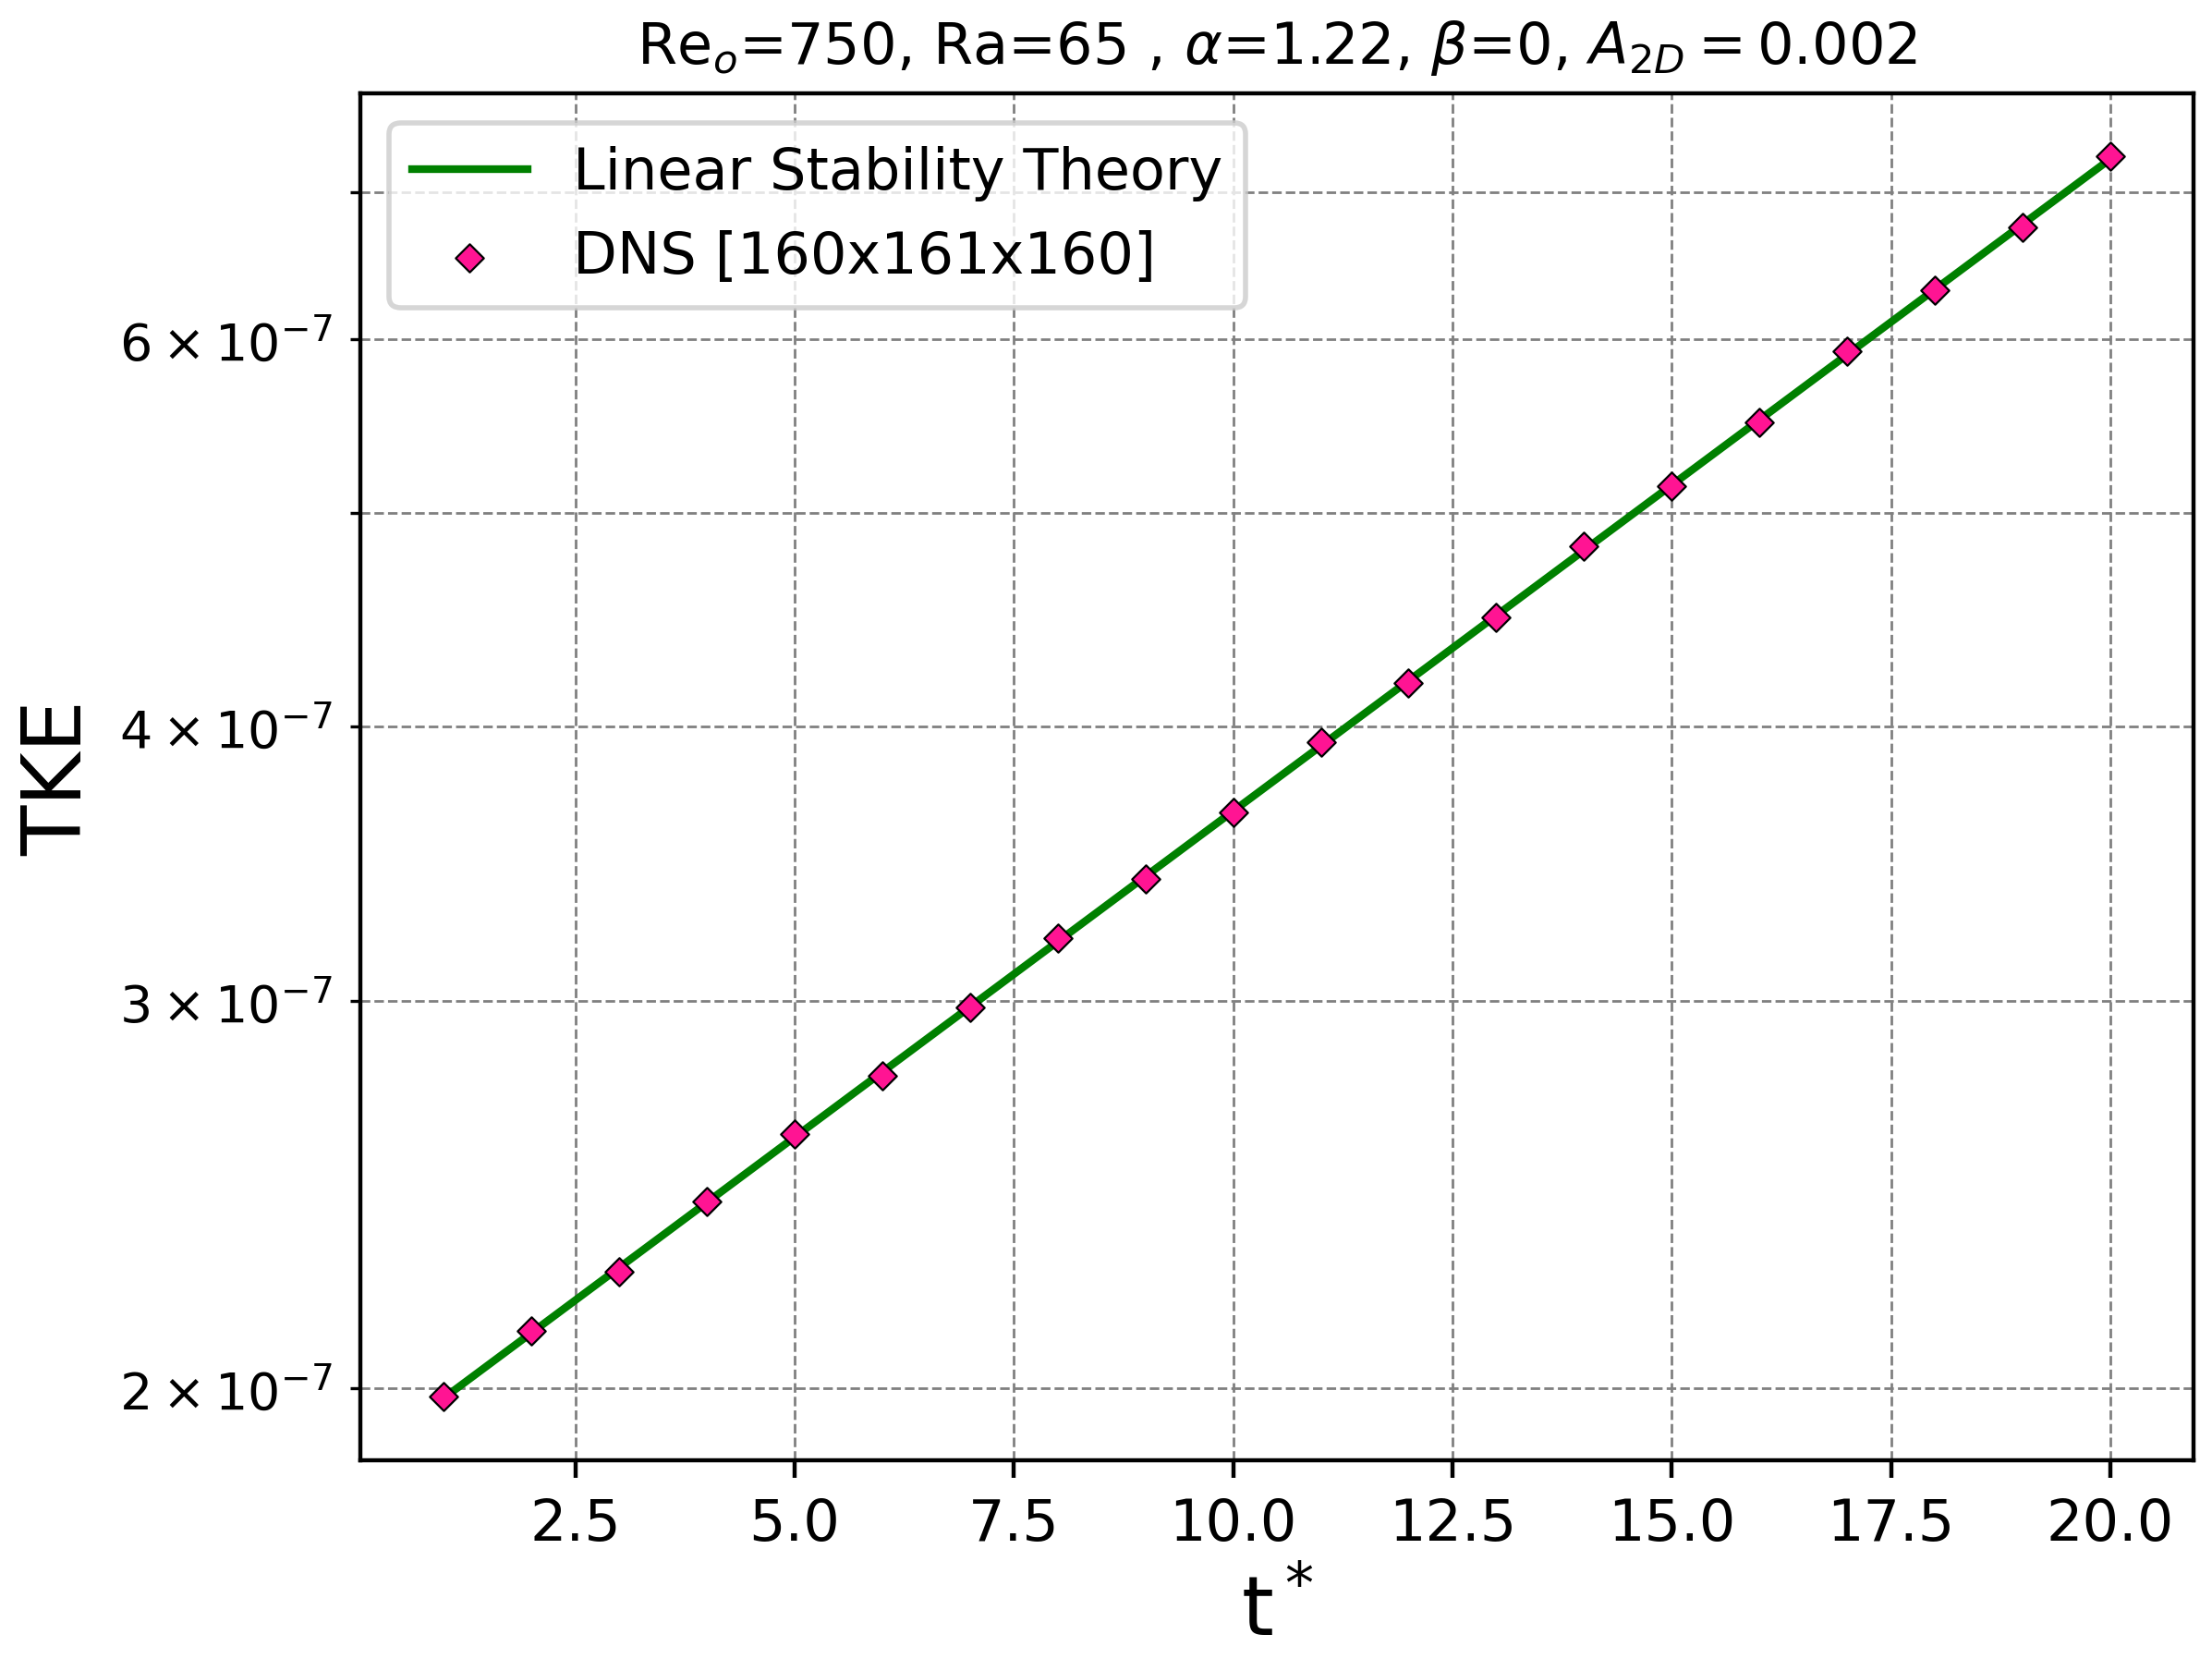
\includegraphics[width=0.49\textwidth]{figures/cap4/osmc/Ra65_RamaDer/tke.png}
    	\label{fig:Ra65RD-tke}}  
  \subfloat[]{
    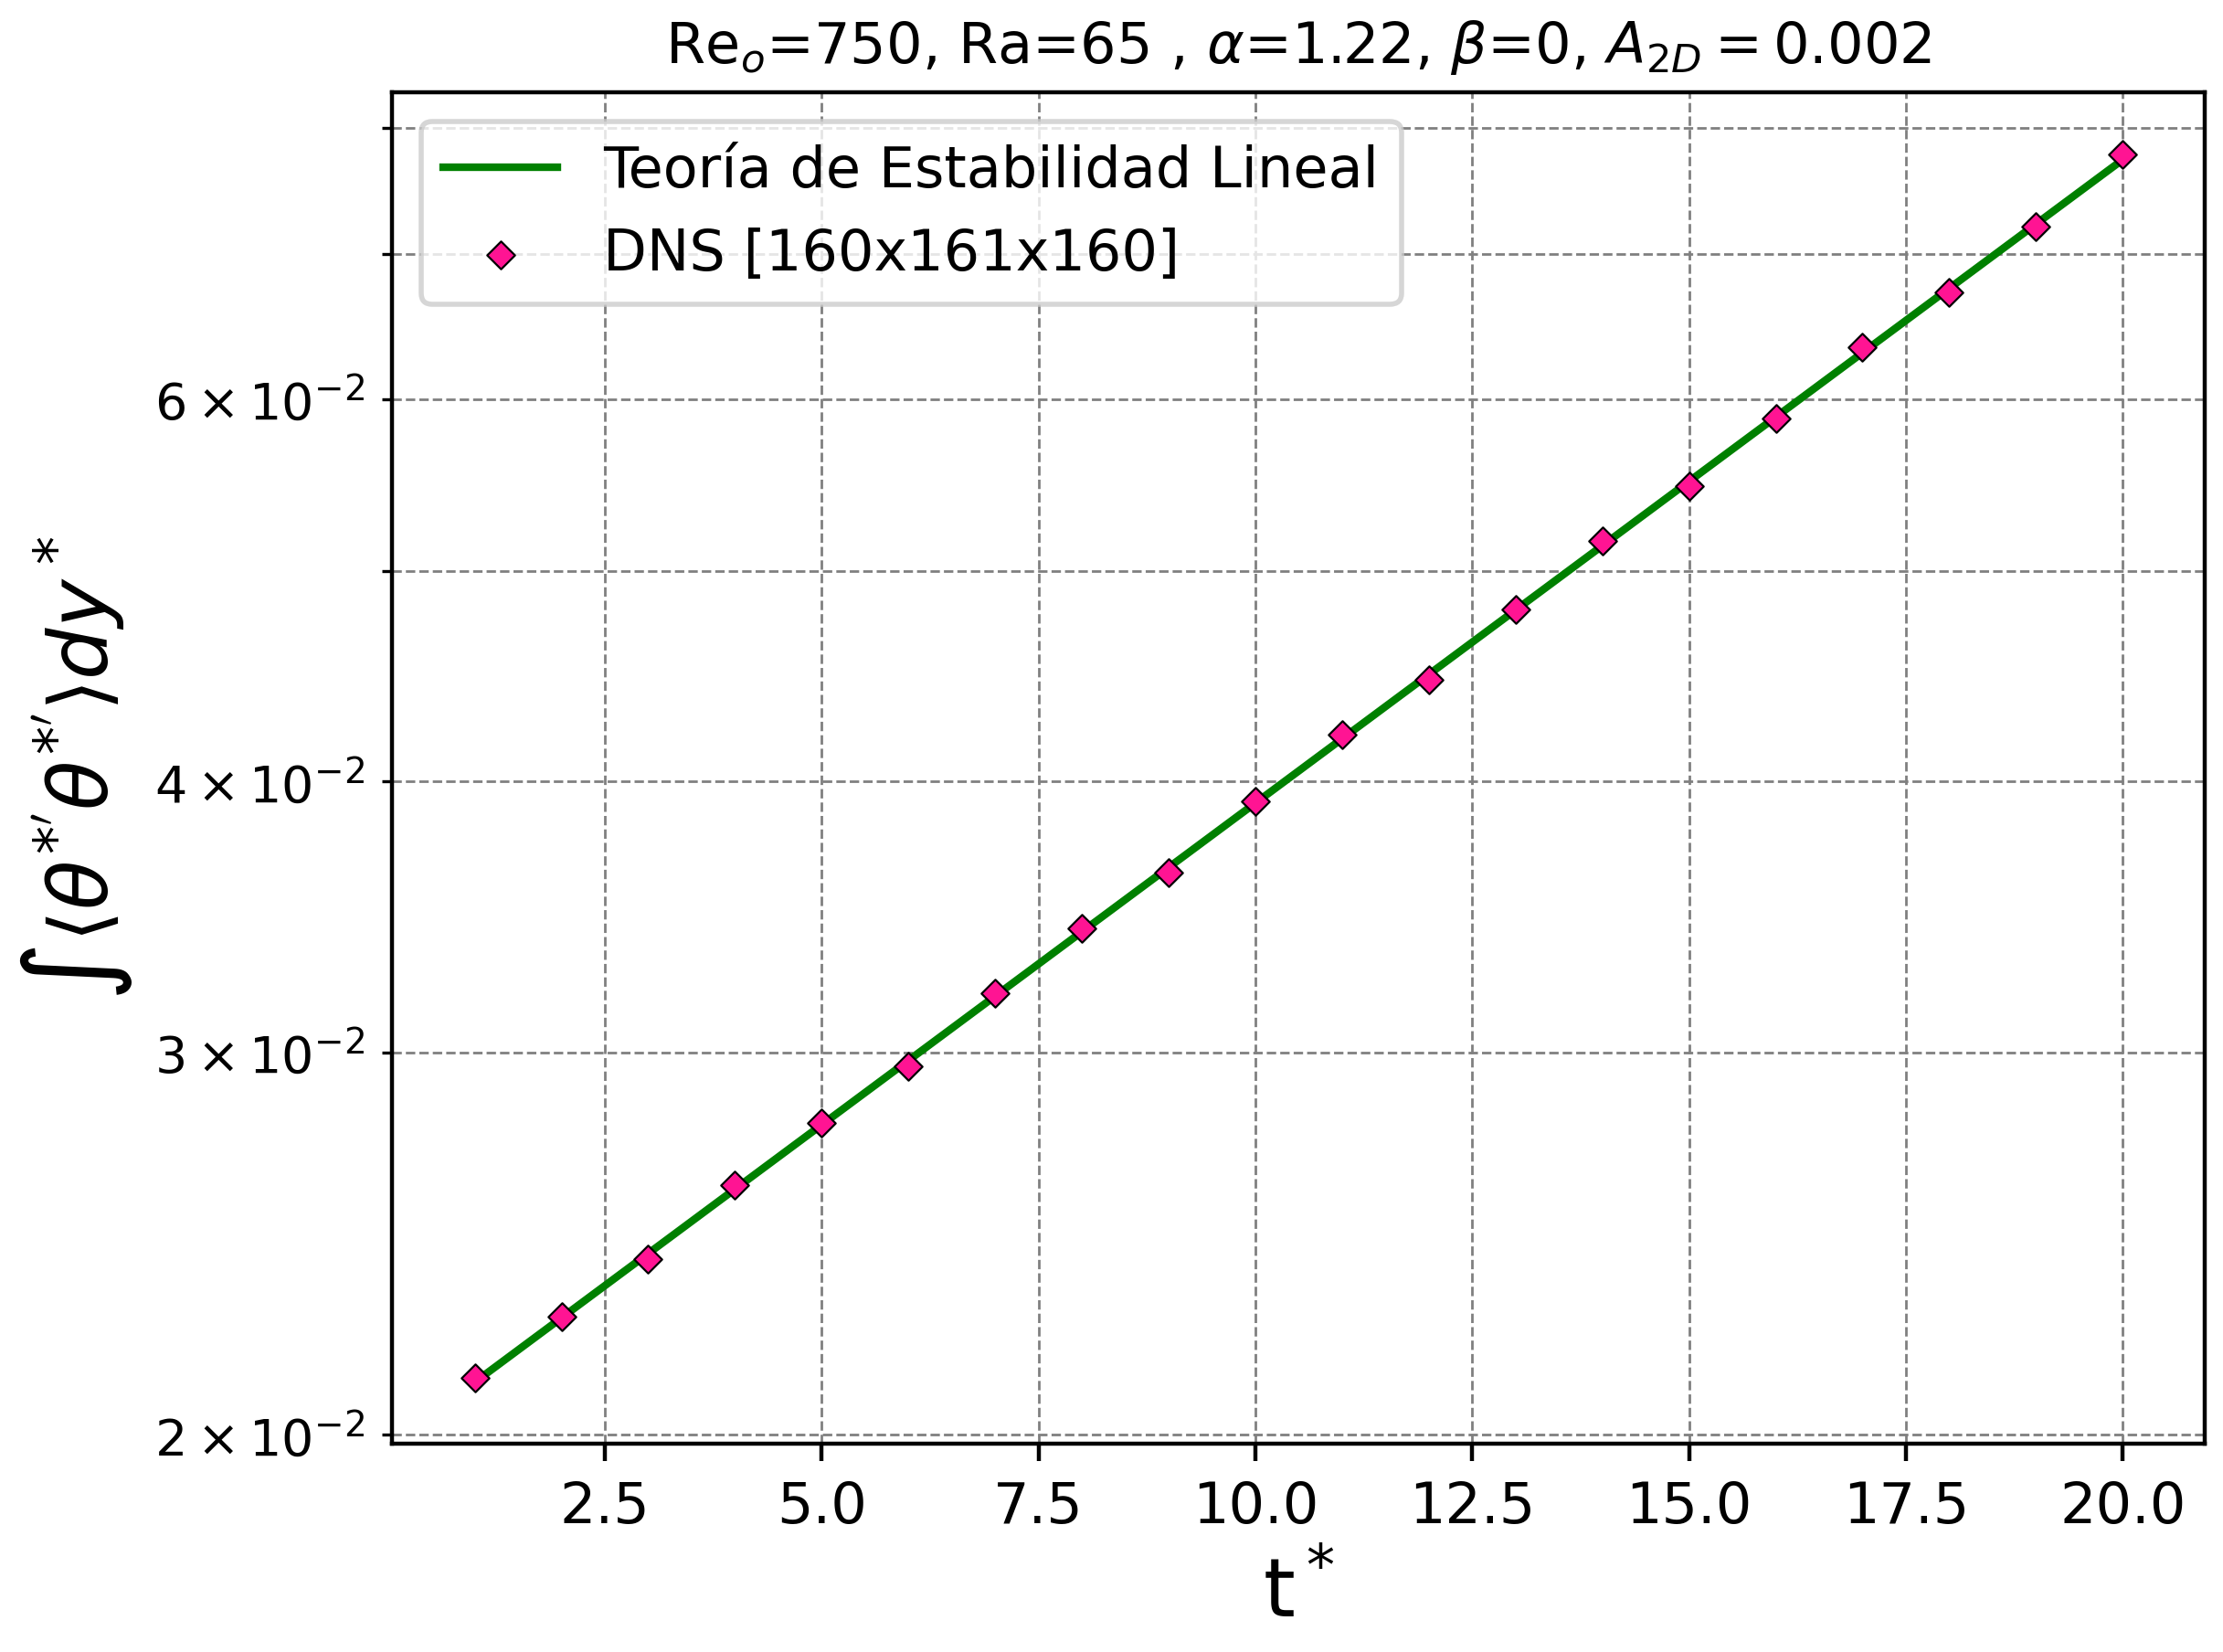
\includegraphics[width=0.49\textwidth]{figures/cap4/osmc/Ra65_RamaDer/theta_var.png}
    	 \label{fig:Ra65RD-tvar}}  
 \caption{Evolución temporal de la TKE y de la varianza de la temperatura del caso RD.} 
 \label{fig:Ra65R-DI}
\end{figure}

\begin{figure}[H]
 \centering
  \subfloat[]{
    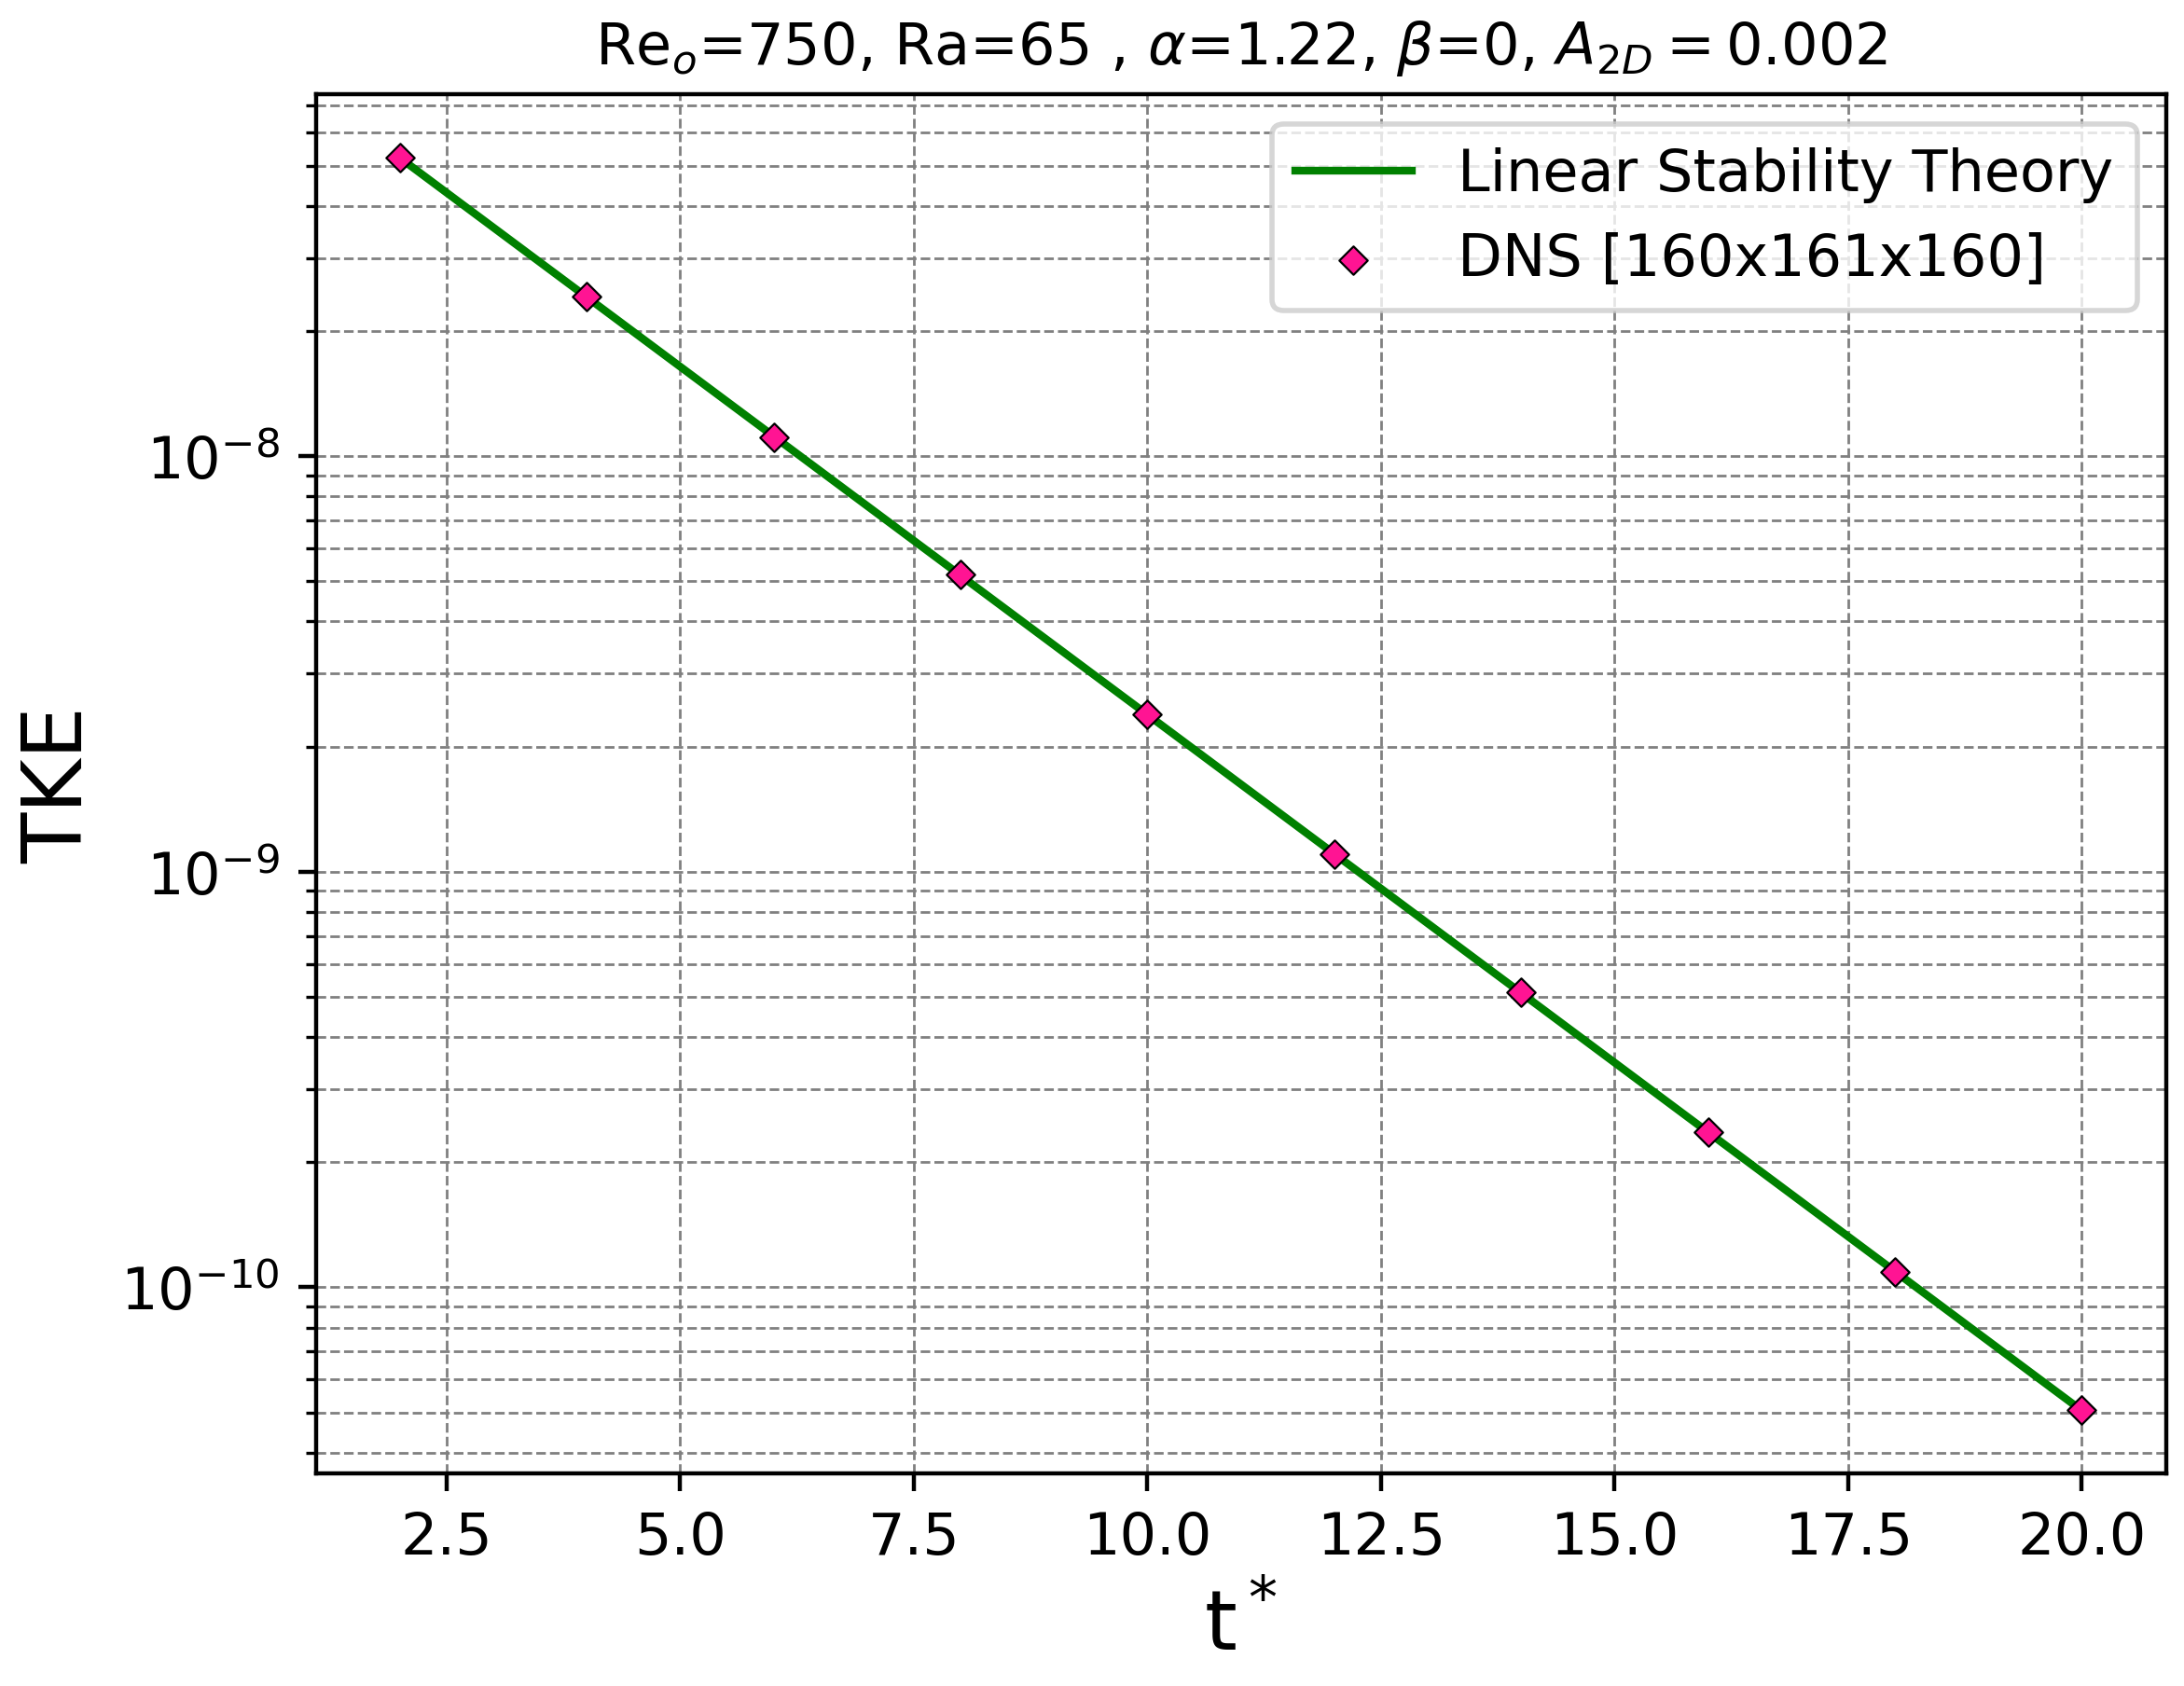
\includegraphics[width=0.49\textwidth]{figures/cap4/osmc/Ra65_RamaIzq/tke.png}
    	\label{fig:Ra65RI-tke}}  
  \subfloat[]{
    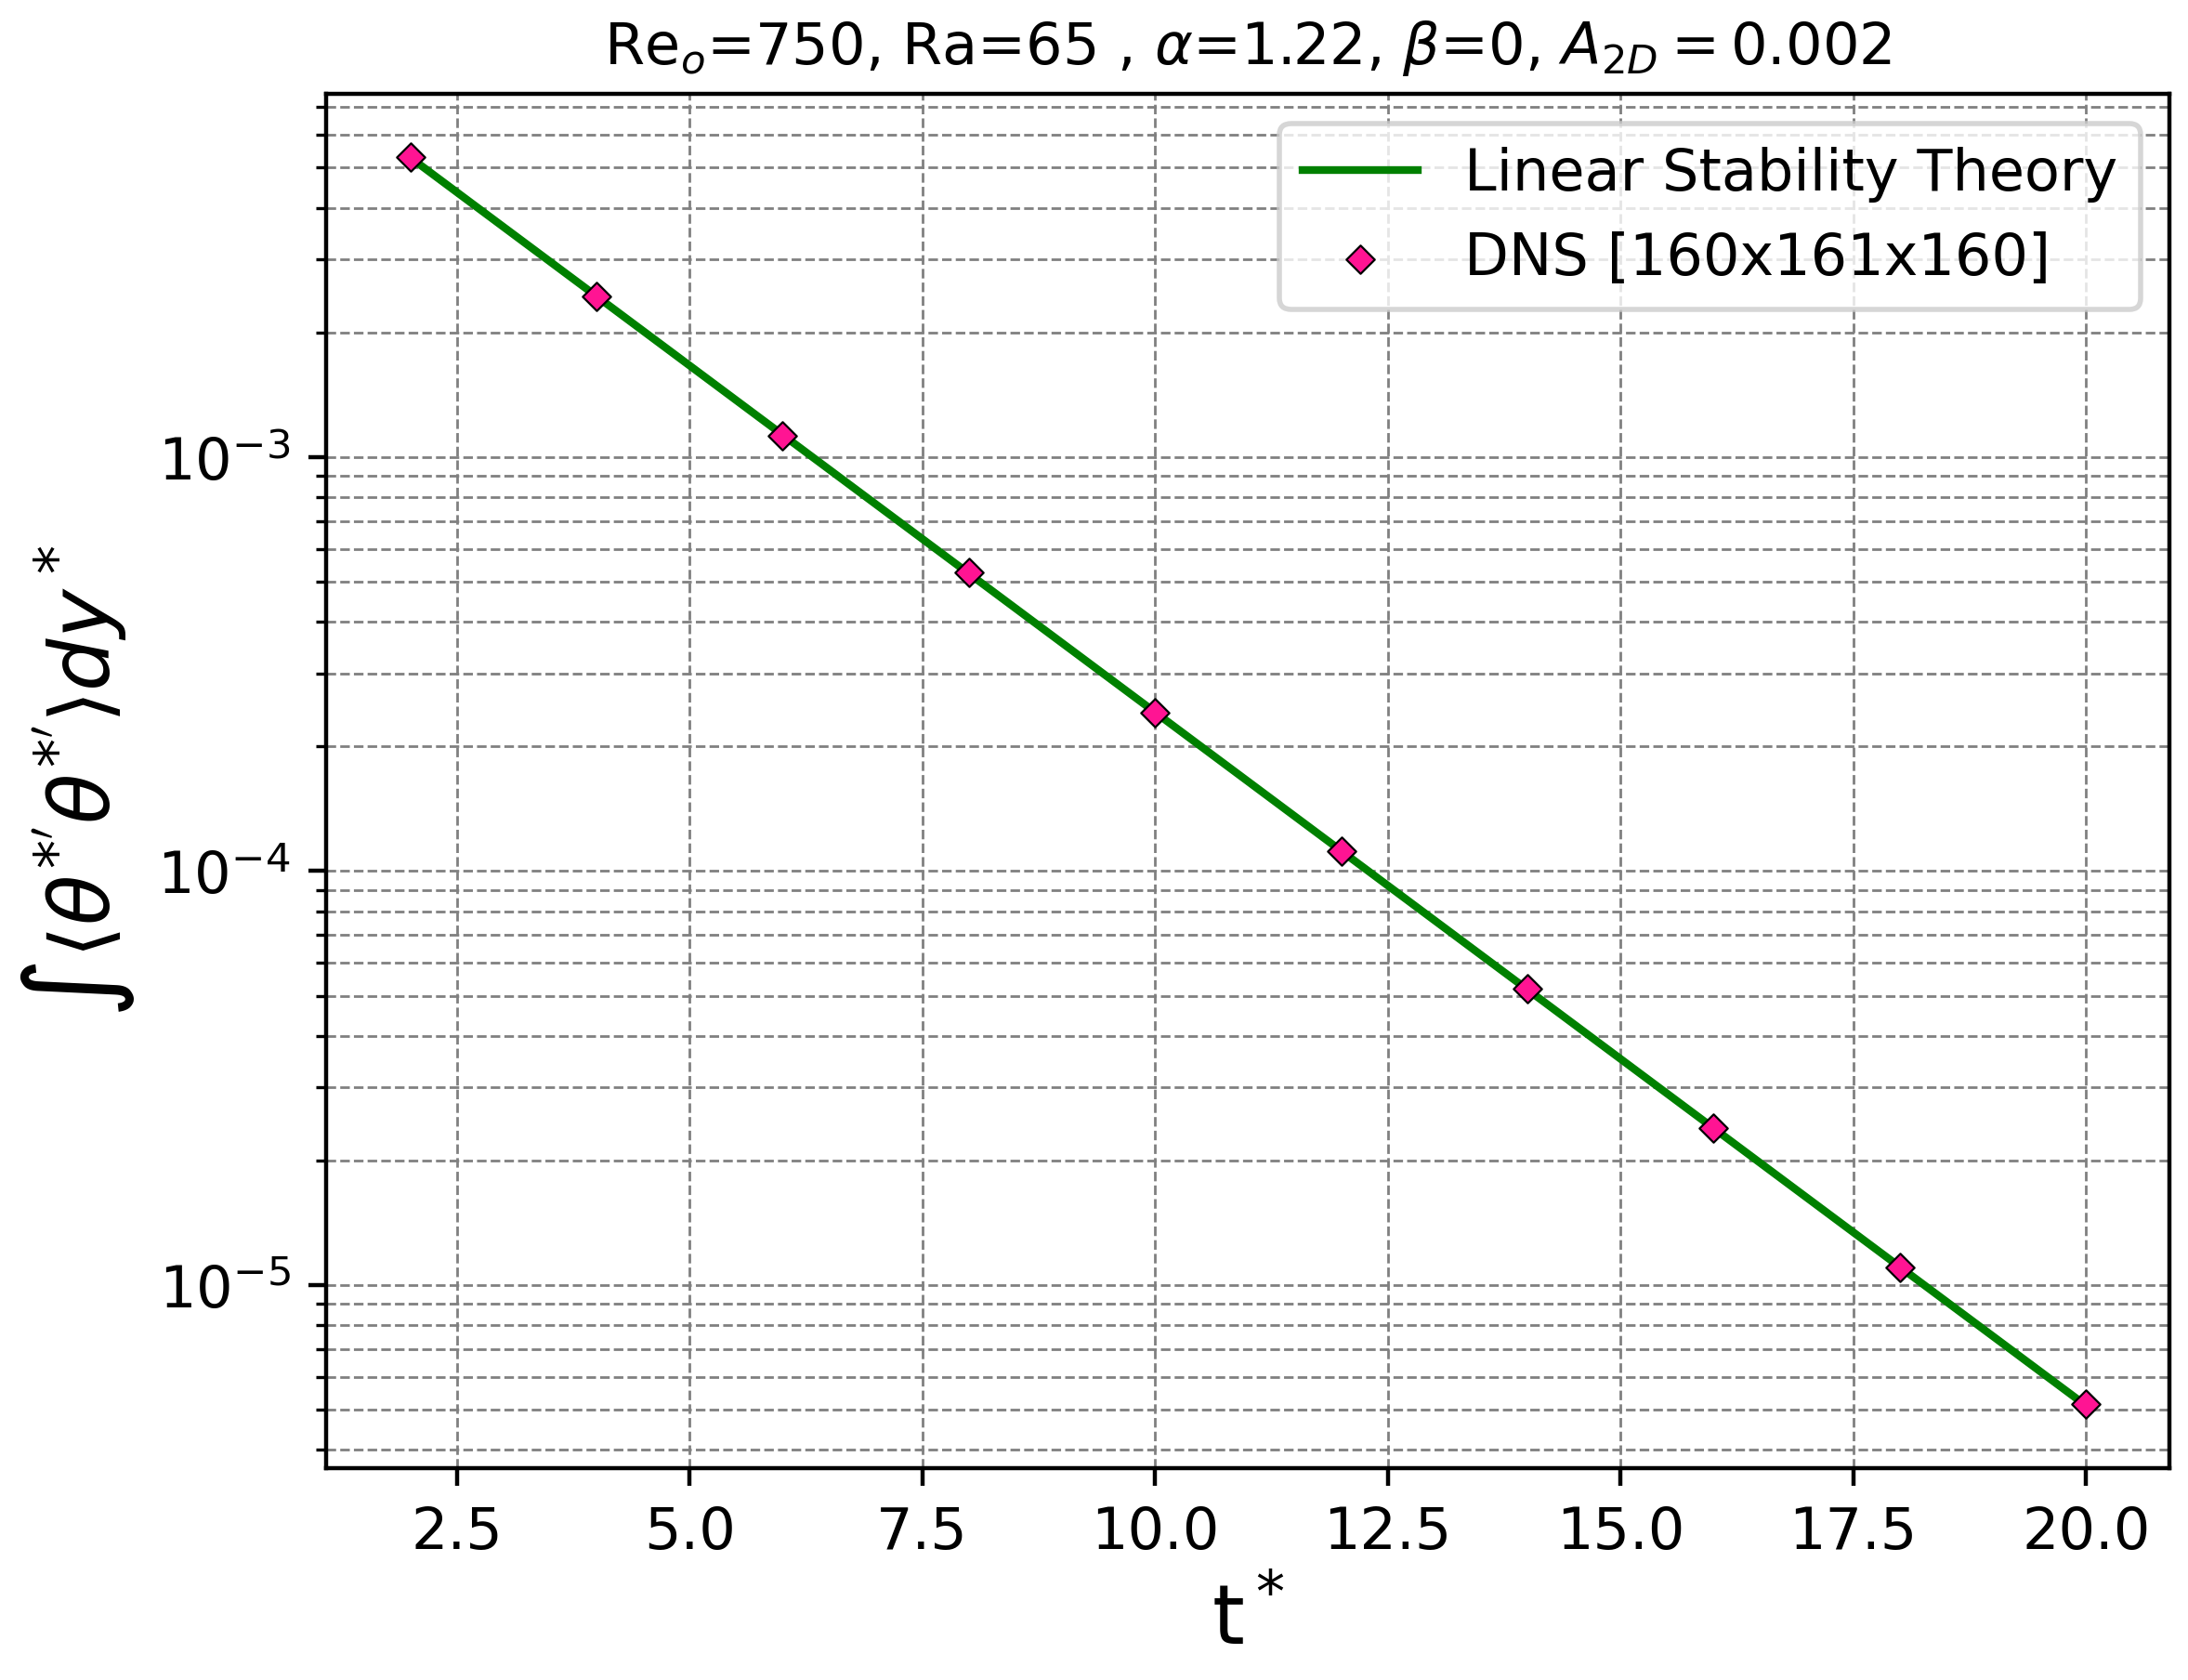
\includegraphics[width=0.49\textwidth]{figures/cap4/osmc/Ra65_RamaIzq/theta_var.png}
         \label{fig:Ra65RI-tvar}}  
 \caption{Evolución temporal de la TKE y de la varianza de la temperatura del caso RI.} 
 \label{fig:Ra65R-DI}
\end{figure}

Finalmente, se puede aseverar que la herramienta OSMC desarrollada por Szuban \linebreak \cite{szuban2023} es adecuada para imponer perturbaciones basadas en la teoría de estabilidad lineal. Por su parte, la herramienta numérica Xcompact3D produce resultados que se encuentran en consistencia con aquellos predichos por la teoría antes mencionada. Esto permite realizar el estudio de la transición temporal laminar-turbulenta que se lleva a cabo en el Capítulo \ref{cap:transicion}.
